\documentclass[12pt,a4paper]{report}

%------------------------------------------------------------------------
% PACKAGES:

\usepackage{lmtstyle}
% Define typearea
% a) Use automatic:
\usepackage[BCOR1cm]{typearea}
% b) Or use fixed:
%\usepackage{geometry}
%\geometry{left=1.5cm,textwidth=18.5cm,top=1.5cm,textheight=26.5cm}
\usepackage[american,ngerman]{babel}
% Use list of tabels, etc. in table of contents:
\usepackage{tocbibind}
% German paragraph skip
\usepackage{parskip}
% Encoder:????
\usepackage[latin1]{inputenc}
%\usepackage[applemac]{inputenc}
% Use A4-paper efficiently:
\usepackage{a4wide}
% Index-generation
\usepackage{makeidx}
% Einbinden von URLs:
\usepackage{url}
% Include .eps-files (needed also for the TUM-logo):
%\usepackage{epsf}
% Special \LaTex symbols (e.g. \BibTeX):
\usepackage{doc}
% Include Graphic-files:
%\usepackage{graphics}
% Include Graphic-files:
\usepackage{graphicx}
%%Added by me
\graphicspath{{images/}}
\usepackage{gensymb}
\usepackage[hidelinks]{hyperref}
\usepackage{amsmath}
\usepackage{caption}
\usepackage{subcaption}
\usepackage{cleveref}
\usepackage{adjustbox}
\usepackage{multirow}
\usepackage{tabularx}
\newcolumntype{Y}{>{\centering\arraybackslash}X}
% Include doc++ generated tex-files:
%\usepackage{docxx}
% Include PDF links
%\usepackage[pdftex, bookmarks=true]{hyperref}
%------------------------------------------------------------------------

%\graphicspath{{figures/}}

%########################################################################
% CHOOSE DEFAULT LANGUAGE:
%\setlang{de}
\setlang{en}

% FILL IN ACCORDINGLY:
\title{Face Tracking for Optimized Bitrate Control in Low Delay Video Encoding}
\type{M} % / M:Master /B:Bachelor / D:Diplom / S:Studienarbeit
\author{Chethan Ningaraju}
\matrikelnr{0365491}
\street{SchrofelhofStra�e 10-05-07}
\town{81375 Munich}
\advisor{Dr.-Ing. Eugen Wige and Mr. Muhammad Zafar Iqbal}
\datebegin{15/07/2016}
\dateend{15/01/2017}
%########################################################################


\begin{document}%****************************************************

\makemtgtitle

% MAIN PART:
\pagenumbering{roman}
% German abstract:
%\switchlanguage{de} % The Kurzfassung, if given, is supposed to be in German!

\thispagestyle{plain}

\section*{Kurzfassung} 
In der Kurzfassung werden auf einer halben Seite das Problemfeld und
die pr�sentierten Ergebnisse zusammengefasst.

\switchlanguage{\lang} % Switch back to the docmuent's default language.
% English abstract:
%\switchlanguage{en} % The abstract is supposed to be in English!

\thispagestyle{plain}

\section*{Abstract}
In video communication applications, coding artifacts are especially disturbing in the face region at low bitrates. In this work, region-of-interest (ROI) based encoding techniques are proposed to preferentially code the face region with a higher quality to improve the perceived visual quality of the video conferencing system. The face region is detected in the video stream and marked as ROI before encoding. 

The low-delay bitrate control proposed for H.264 video coding standard is extended to implement two different approaches of ROI-based encoding. In the first approach, QP offsets for ROI is computed based on the relative area of ROI to reduce the quantization parameter (QP) allocated for ROI macroblocks. In the second approach, region-based bit-allocation is performed to allocate a higher proportion of bits to ROI macroblocks. The two approaches offer a tradeoff between complexity and output quality. In contrast to the previous ROI-based video coding approaches, this work uses the complexities of ROI and non-ROI parts in a video frame to allocate an optimal amount of bits for the corresponding regions. Experimental results demonstrate that the quality of ROI is improved without any noticeable degradation in non-ROI quality hence improving the overall perceived visual quality at low bitrates.

In addition to ROI-based coding, optimization techniques are proposed for real-time face detection in a video stream by reusing motion vector information computed during motion estimation stage of video encoding. This work proposes motion vector based variable interval face detection technique instead of detecting the face in every frame of the video. The motion vectors of face regions are analyzed to perform face detection only when there is movement in the face region.

%\switchlanguage{\lang} % Switch back to the document's default language.

% Table of contents:
\tableofcontents 

% Introduction (Einleitung):
\chapter{Introduction}
\pagenumbering{arabic}%Ab hier, werden arabische Zahlen benutzt
\setcounter{page}{1}%Mit Abschnitt 1 beginnt die Seitennummerierung neu.
\thispagestyle{empty}

%Die Einleitung soll zum eigentlichen Themengebiet hinf�hren und die
%Motivation f�r die Arbeit liefern. Am Schlu� der Einleitung wird
%weiterhin noch eine �bersicht �ber die restliche Arbeit gegeben.
In recent years, there is increasing demand for high-quality video conferencing solutions. Due to availability of high-speed internet, video conferencing has proved to be an efficient alternative to face-to-face meetings. Video telephony has grown into a multi-billion dollar industry and has huge commercial significance. To address this growing need there has been constant improvement in  low-delay video coding techniques in addition to better techniques to ensure low-delay transmission reliability at the network level. The tremendous increase in smartphone usage has led to an increase in video telephony over cellular networks whose bandwidth is highly constrained. Therefore, it is very important to develop methods of delivering high quality video with less bandwidth requirement. 

The most commonly used video coding standards like H.264/AVC have been designed to exploit the spatial and temporal redundancies in the input video stream to achieve high data compression. The techniques of spatial and temporal prediction form the core principle of these video coding standards \cite{h.264-overview}. However, after encoding the video the perceptual redundancies still remain since human attention does not focus on the whole scene but only a small region of fixation called region-of-interest (ROI) \cite{Perception-model-of-face}. Therefore, reducing the perceptual redundancy gives a new dimension towards achieving lower bit-rate at acceptable perceptual quality. This work proposes a region-of-interest based bitrate control scheme for low-delay video encoding to exploit the perceptual redundancies.

In this work, the salient region of the frame which is the face of the participant in a video conference is identified. Since the attention of the viewer is mostly focused on the face of the other participants during a video conference call, improving the quality of the face region (ROI) can improve the overall perceptual quality. In this work, ideal capture conditions are assumed and results of the face tracking is used directly as supplementary information for the H264/AVC encoder's bitrate control. This work explores the methods of region of interest(ROI) based encoding to exploit the available bandwidth to encode regions that are of high importance to perception with higher quality. Face region in the input stream is allocated an above-average bit-count to yield a better visual quality than the background regions. It is the aim of this work to develop and extensively evaluate the strategy of uneven bit-allocation and also to identify its limitations.

The remainder of this thesis is organized as follows. Chapter \ref{chapter:Background} gives an overview of the hybrid video coding used in H.264, functionality of the bitrate control module and the concept of Region-of-Interest(ROI) based encoding. In Chapter \ref{chapter:Literature_survey}, a literature review is presented which discusses related earlier research works in the field of ROI-based encoding. An insight into limitations of the earlier works is also presented in this chapter. A detailed overview of the low-delay bitrate control module \cite{JVTF086} used in this work is presented in chapter \ref{chapter:used-bitrate-control-overview}. Chapter \ref{chapter:study_setup} deals with explanation of the setup used in this work along with assessment techniques to evaluate ROI-based encoding approaches presented in this thesis work. The proposed bitrate control for ROI-based encoding is presented in Chapter \ref{chapter:ROI-RC}. The conclusion for this thesis work along with a note on potential future work related to this topic is presented in chapter \ref{chapter:conclusion}.





% Text Body (Hauptteil)
% Could have multiple chaper-files, e.g.:
\chapter{Background} \label{chapter:Background}
\thispagestyle{empty}% no page number in chapter title page
A brief overview of principles of hybrid video coding used in H.264 is presented in this chapter. The ROI-based encoding approaches discussed in this work are implemented in the form of intelligent bitrate control schemes. Therefore, an overview of the bitrate control module is presented to provide the reader with an understanding of the functionality of bitrate control in a video encoder. Finally, the concept of ROI based encoding is introduced.

\section{Hybrid Video Coding}
H.264/AVC is one of the most commonly used video coding standard. Figure \ref{fig:Hybrid Video Coding} depicts the underlying principle of block-based hybrid video coding used in H.264 \cite{h.264-overview}. The encoding scheme aims to exploit the spatial and temporal redundancies that exist in a video. 


In this coding scheme, the input picture is represented in block-shaped units(16x16 pixels) of associated luma and chroma samples called macroblocks (MBs). The basic source-coding algorithm is a hybrid of inter-picture prediction to exploit temporal statistical redundancies and transform coding of the prediction residual to exploit spatial statistical dependencies. The two types of prediction used are:
\begin{description}
	\item[Intra Prediction:] There exists a high similarity among the neighboring blocks in a video frame. In intra prediction, a block is predicted from its neighboring pixels of already coded and reconstructed blocks. H.264 offers nine intra prediction modes (one DC prediction mode and eight directional prediction modes) \cite{h.264-overview}.
	\item[Inter Prediction:] When the frame rate is sufficiently high, there is a great amount of similarity between neighboring frames. It is highly efficient to code the difference between such similar frames than the frames themselves. In inter prediction, block-based motion estimation (ME) is used to predict the motion of macroblocks relative to the previous encoded frames.
\end{description}

The first frame in a video is encoded using intra prediction and transform coding. The transform coefficients are quantized to achieve high compression ratio. The frames which are encoded without any dependencies on the neighboring frames are called key/intra frames, and act as reference frames to encode subsequent frames.

Once a reference frame is available, inter prediction can be used to remove the temporal redundancies. During motion estimation, it is usually not possible to find an exact match for the current macroblock. Therefore, the residual error is estimated for the prediction from motion estimation. This is called motion compensation. The residual error is coded using transform coding followed by quantization to achieve higher compression ratio. Due to quantization, it is not possible to recover the exact transform coefficients at decoder end without any loss of information. This introduces distortion in the decoded frame.

These frames which are predicted from other reference frames are called inter frames. The inter frames which use only past frames as reference are called P-frames. In addition to past frames, future frames can also be used as reference. Such frames are called Bi-directional frames or B-frames. Both B-frames and P-frames can be used as reference frames for encoding subsequent frames.

The quantization step used to quantize transform coefficients is specified using quantization parameter (QP). In H.264, QP range of 1 to 51 is allowed which is translated to quantization steps. The magnitude of distortion introduced by quantization depends on the quantization parameter. A lower QP implies low quantization step resulting in high quality output with less compression. The compression ratio increases with increase in QP at the cost of decreased output quality. The output data rate of the encoder is controlled by computing suitable QP, this is the task of bitrate control module as described in the following section. A detailed overview of individual steps involved in H.264 coding can be found in \cite{h.264-overview}. 

\begin{figure}[h!]
	\centering
	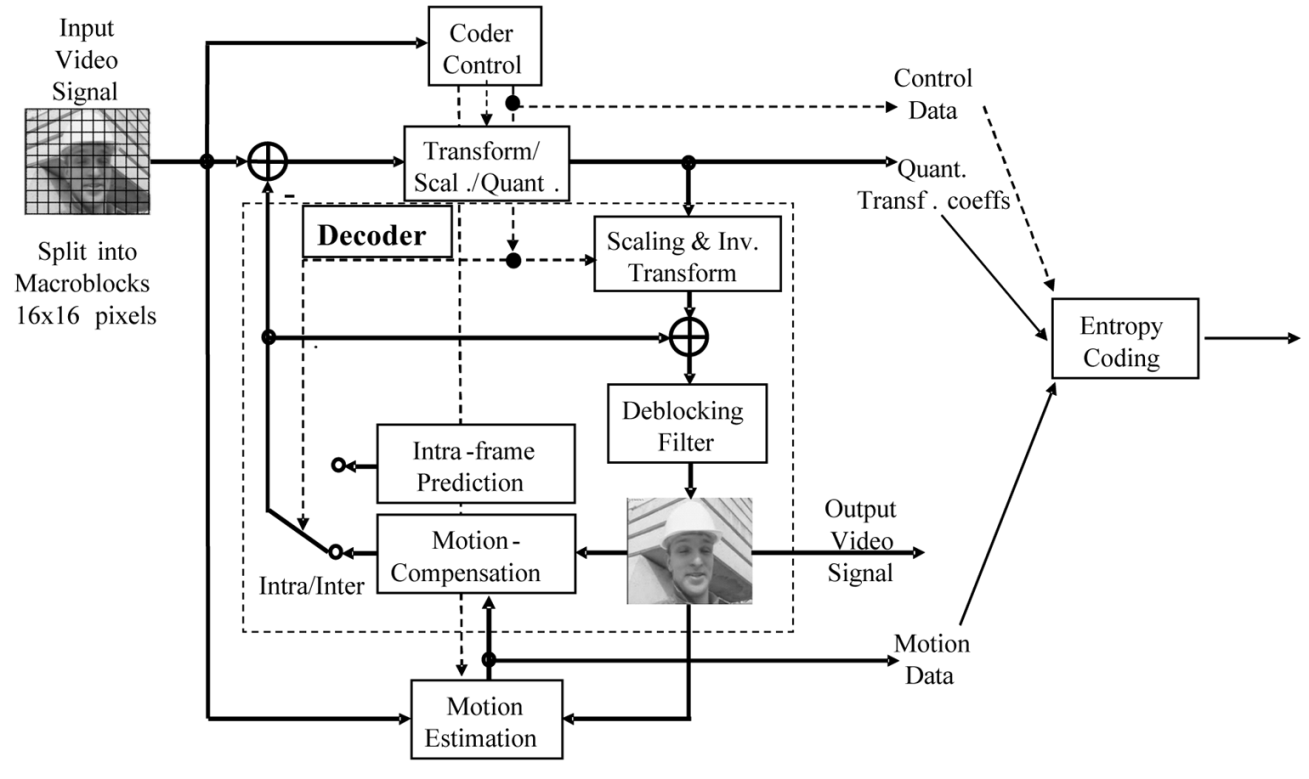
\includegraphics[scale=0.5]{general/Hybrid_video_coding.png}
	\caption{Block-based hybrid video coding\cite{h.264-overview}}
	\label{fig:Hybrid Video Coding}
\end{figure}

\section{Bitrate Control} \label{Intro:Bitrate-Control}
The bitrate control module is responsible for controlling the bit-consumption of the encoder to guarantee smooth playback. Bitrate control is not specific to a video coding standard and hence operates independent of any chosen video coding standard. There are various flavors of bitrate control like Constant Bitrate (CBR), Variable Bitrate (VBR) and Average Bitrate (ABR). In this work, CBR type of bitrate control is considered since it is most commonly used in video conferencing and other real-time streaming applications. 
\begin{figure}[h]
	\centering
	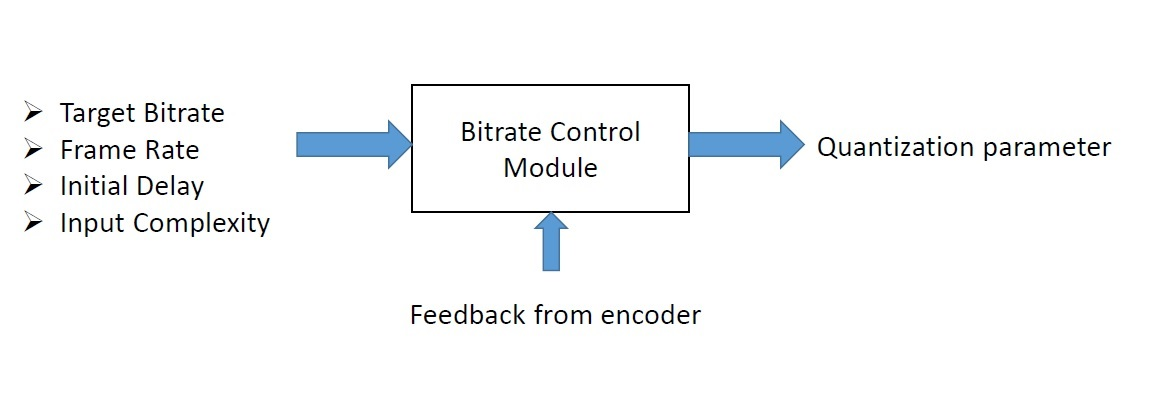
\includegraphics[scale=0.5]{RC_block}
	\caption{Bitrate Control Module Functionality}
	\label{fig:Bitrate Control Module Functionality}
\end{figure} 

\begin{figure}[h]
	\centering
	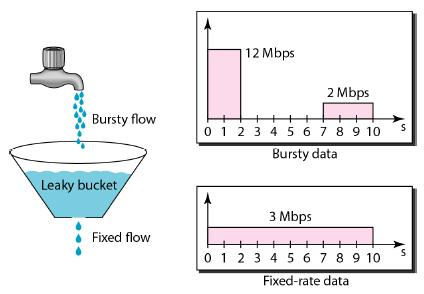
\includegraphics[scale=0.5]{general/Leaky_bucket}
	\caption{Leaky Bucket Model\cite{Leaky-bucket-NSI}}
	\label{fig-Leaky-Bucket-Model}
\end{figure} 	
Figure \ref{fig:Bitrate Control Module Functionality} illustrates the functionality of the bitrate control module. The main purpose of bitrate control module is to ensure smooth playback of the encoded video under given bandwidth and delay constraints. It estimates the video bitrate based on the available network bandwidth, ensures that the coded bitstream can be transmitted within the specified delay and makes full use of the limited bandwidth \cite{InTech-Rate-control-in-video-coding}. It achieves this by controlling the QP used during the encoding. The QP is computed considering the input bitrate, framerate, input complexity (spatial and temporal activity) and acceptable delay of the system. The module also receives regular  feedback from the encoder to make better QP adaptation.  The feedback from the encoder gives information about the complexity of the input video and helps the bitrate control to compute optimum QP for a given bit-budget.

The functionality of the bitrate control module can be illustrated with the help of the leaky-bucket model \cite{InTech-Rate-control-in-video-coding}. The output data rate of a video encoder varies depending on the input complexity of the video (motion in the frame). It also depends on the picture type of the encoded frame. The key/I-frames consume a lot of bits compared to inter pictures (P-frames and B-frames). In a video streaming scenario considering a constant bitrate channel, the throughput is maximum when data-rate is constant and equal to the available bandwidth. Therefore, the output data of the encoder is smoothened using a theoretical buffer called Video Buffer Verifier (VBV). The VBV is a virtual buffer modeled by the bitrate control module to ensure that the video stream can be correctly buffered and played back at the decoder end. This is equivalent to the leaky-bucket model as shown in Figure \ref{fig-Leaky-Bucket-Model} \cite{Leaky-bucket-NSI}, where the output of the encoder with a variable rate (bursty output) is stored in a buffer (leaky bucket) which is draining at a constant rate.  Any underflow or overflow of this buffer causes glitch in the video streaming. To ensure that there is no VBV overflow or underflow, encoder's quantization parameter is adapted on a macroblock level so that the maximum allowed bit-count for an encoded frame is not exceeded. A detailed description of the low-delay bitrate control module used in this work is given in chapter \ref{chapter:used-bitrate-control-overview}.

\section{ROI-based Coding}

In conventional video coding, all regions of a frame are considered equally important to the viewer. It is assumed that all regions contribute equally to the perceptual quality. However, the study of Human Visual System (HVS) shows that human eyes can only focus on one area in a frame at any given time which is called region of interest. For example, it has been found out in \cite{human-vision-proof-NSI} that humans normally perceive clearly a small region of 2\degree-5\degree of the visual angle. This corresponds to a very small region in a video frame.

In video coding, the compression gain from spatial and temporal prediction is reaching saturation level. Further compression from these techniques demand exponential growth in computational capabilities. The next generation video coding standards like HEVC/H.265 claims to offer two fold increase in compression ratio over H.264. This increase in compression comes with multi-fold increase in computation complexity during encoding \cite{H264-HEVC-comparison}. Therefore, perceptual coding can provide an alternative solution towards lower bitrate video coding. The technique of encoding regions with higher importance to perceptual quality at a higher quality at the cost of degradation of quality in non-ROI parts is called ROI-based coding. The loss of quality in non-ROI is not perceived by the viewer leading to increased perceptual quality at the same bitrate.

%Some of the commonly used video codecs use the fact that high frequency components are less important to the human visual system and perform preferential coding based on spatial frequency. The high frequency components which are not so important to the perceptual quality are encoded with a higher QP. However, such preferential coding does not take into account the region of interest to the viewer in the frame to be encoded. All high frequency components are coded with higher quantization irrespective of the region belonging to ROI. 

The ROI-based coding is not a common practice in video coding because it is very hard to automatically detect important regions in generic contents that contribute the most to the perceptual quality. There are many ways of detecting region of interest, most of which are application specific. The most common approach is usage of difference image based moving object detector. In these systems any moving object is considered as ROI. A typical use-case for such a system is video surveillance. In addition to difference image based motion detection, global motion estimation is used in ROI detection \cite{ROI-aerial-surveillance} in applications like aerial surveillance.

In generic video content, ROI changes constantly depending on the context. For instance, in a movie, the ROI can depend on context of the scene. Developing generic techniques for detection of ROI in such videos is very difficult. There have been attempts to use eye tracker to record the foveation points of a human observer on the receiver which was used to apply foveation filter in video coding of the sender. An advancement over such approach is proposed in \cite{foveated-rate-control} which optimizes rate control to maximize foveal visual quality metric. These generic ROI detectors are very hard to implement due to uncommon availability of eye tracking mechanism at the receiver. 

The region of interest in the video conferencing scenario is going to be the face region predominantly. Due to recent improvements in face detection algorithms it is possible to detect the face with good accuracy. The study in \cite{HighQualityROICodingForVideoConferencing} shows that boosting quality of the face regions can improve the overall perceived quality of the video. This work aims to study possible ways of improving perceptual quality of the video by detecting face region and coding it with higher quality than rest of the frame.

%%To be moved to after ROI-based coding
In conventional video coding, the bitrate control allocates bits at every macroblock and adjusts the QP accordingly. In a simple approach, every macroblock is considered equally important to perceptual quality hence the available bits are distributed evenly across all macroblocks within a frame. Since low-latency and load efficiency are of high importance it is not advisable to do multi-pass encoding for optimal bitrate allocation. Therefore, over-allocation in one macroblock has to be compensated by under-allocation (using a higher QP) for neighboring macroblocks, regardless of the image content. However, a more intelligent allocation strategy should take the image content into account. In this work, parts of the image with higher importance (ROI) is given a higher share of the overall bit-count resulting in higher visual quality. The additional bits spent in coding ROI is compensated by allocating a lower proportion of the bit-count to the background regions (non-ROI).

The knowledge of region of interest in input video can be used for many other purposes in addition to its use in video coding to improve perceptual quality. For instance, ROI information can be used in developing techniques for smart thumbnail displays in group video conferencing solutions. In a group video conference, an active person is detected based on the source of the voice and is displayed on the main screen and other participants are displayed on the smaller windows with down-scaling of the entire video. If the face coordinates of the participant is transmitted along with the bit-stream as meta-data, a cropped version of video can be displayed to show only the face in thumbnail display. This can improve the overall user-experience.

%% Section to throw light on other works in same field
\chapter{Related Work} \label{chapter:Literature_survey}
\thispagestyle{empty}% no page number in chapter title page
The concept of region of interest based encoding has been around for a while. In this chapter, some of state-of-the-art techniques are discussed. The different approaches of using ROI information to improve perceptual quality can be broadly classified into following categories based on the stage of processing using ROI information.
\begin{itemize}  
	\item Preprocessing - Example: blurring.
	\item Video Coding - Example: during the rate-distortion optimization (RDO), bitrate control.
\end{itemize}
The relevant techniques proposed under these categories are discussed in the following sections.
\section{Preprocessing} \label{sec:Literature_survey_Preprocessing}
The input video stream can be directly altered based on the ROI information. Many pre-processing approaches are also used to directly reduce unimportant information by applying a non-uniform distortion filter in a scene. For instance, the image is divided into foreground (ROI) and background (non-ROI) and the non-ROI parts are blurred to save bits during encoding \cite{ROI-background-blurring}. The work in \cite{pre-postprocessig-ROI-codec-independent} is an example for codec independent ROI encoding. It can work with any codec and arbitrary ROI detector. In this approach, input video stream is modified only to contain relevant information. The non-ROI pixels are replaced such that these regions can be very efficiently compressed by the encoder. The non-ROI macroblocks are either replaced by corresponding blocks from the previous frame or black blocks. The non-ROI regions are reconstructed with post-processing assuming a zero motion vector. This approach is used in scenarios where non-ROI regions are mostly discarded completely at the receiver end.

\section{Video Coding}
In video encoding, multiple approaches exist to preferentially code ROI macroblocks with a higher quality at the cost of degrading non-ROI parts. The ROI information can be directly used in RDO during video encoding to alter the quality of ROI. One such approach is presented in \cite{ROI-rate-control-H264} in which non-ROI macroblocks are encoded using only AMC-based modes (Active MB Concealment). The non-ROI macroblocks are encoded with only motion vector but no residual information. This creates a bias to choose larger distortion for non-ROI blocks to save bits during Lagrangian optimization. The bits saved during encoding of non-ROI macroblocks is used to encode ROI blocks with a higher quality

The resources available during encoding like computational power is preferentially allocated to ROI in \cite{ROI-resource-allocation}. The H.264 coding standard offers many methods to enhance its compression performance such as variable block size ME, quarter-sample-accurate ME, and multiple reference frames ME \cite{h.264-overview}. The complexity of H.264 encoder is significantly increased due to employment of these new methods. The computation need for non-ROI is reduced significantly at the cost of compression efficiency by adaptively adjusting the coding parameters as follows,
\begin{itemize}
	\item Choose only a subset of macroblock partition and prediction modes offered by H.264 standard for non-ROI during rate-distortion optimization to find the best mode. This is similar to usage of only AMC-based prediction modes for non-ROI proposed in \cite{ROI-rate-control-H264}.
	\item The number of reference frames is reduced to use only immediate neighboring frames for non-ROI macroblocks. The ROI MBs are allowed to reference from multiple frames.
	\item The accuracy of subpixel accurate ME is set to quarter-pixel for ROI and half-pixel for non-ROI MBs.
	\item The ME search range is reduced significantly for non-ROI. 
\end{itemize} 
These modifications in coding parameters result in a higher quality for ROI even when the available bit-budget is uniformly distributed across ROI and non-ROI parts. 

A more common way of ROI-based encoding is by altering the rate control module to allocate above average bits to ROI macroblocks. In addition to preferential allocation of computation power to ROI, ROI-based rate control is proposed in \cite{ROI-resource-allocation}. The modifications to the rate control scheme for low-delay video communication of H.264 \cite{ROI-resource-allocation-rate-control} has been proposed to allocate more bits (smaller QP) to the ROI macroblocks. This is done by assigning weights to every macroblock based on its importance to the human visual system. A linear R-Q model is proposed to optimize QP calculation to provide a ROI-based rate control at the MB level.

The work in \cite{ROI-bit-allocation-h264} proposes a bit-allocation and rate control scheme for enhancing regional perceptual quality using structural similarity(SSIM) index as the quality metric for distortion-quantization modeling. Statistical analysis is adopted to obtain the relation between SSIM of reconstructed MBs and corresponding QP (from 20 to 51 in this paper) after standard video coding. A target SSIM is set for the ROI and corresponding QP is determined with the help of the SSIM-QP model. The proposed algorithm has following steps.
\begin{itemize}
	\item Target bits for each basic unit is estimated and allocated based on the bit-budget of ROI or non-ROI parts.
	\item A preliminary QP for each BU is computed based on R-Q model.
	\item The predicted QP is used for rate-distortion optimization mode decision of the encoding flow to obtain the best prediction macroblock.
	\item The QP for MBs in ROI used for final encoding is altered to achieve the target SSIM quality based on the SSIM-Q model
\end{itemize}

A ROI-based encoding scheme specific to video conferencing is proposed in \cite{ROI-MV-based-face-tracking} for H.263. This work proposes an algorithm to track the face using motion-vector information. Once the ROI is detected, it proposes modification of bit-allocation for both CBR and VBR mode of rate control. The QP for these blocks is predicted from the rate modeling of ROI and non-ROI blocks. The work described in \cite{Perception-model-of-face} goes a step further in face detection based ROI encoding schemes by enhancing finer facial feature to improve the perceptual quality in high-resolution HEVC encoding. In this approach, different weights are assigned to the background, face, eyes, mouth and nose regions which are in-turn used to alter quality by ROI-based adaptive CTU (Coding Tree Unit) partition structure for HEVC.

\section{Inference}
The preprocessing based ROI encoding approaches described in section \ref{sec:Literature_survey_Preprocessing} \cite{ROI-background-blurring, pre-postprocessig-ROI-codec-independent} offers codec independent ways to enchance quality of ROI. However, these approaches are not suitable for video conferencing since they can cause a very high degree of degradation in the background regions (non-ROI) due to preprocessing. An excessively degraded background can also reduce the perceptual quality. It also needs an additional stage of preprocessing which adds to the complexity of the system making it hard to process in real-time.

The proposed bitrate control schemes for ROI-encoding \cite{ROI-MV-based-face-tracking,ROI-resource-allocation-rate-control} assign arbitrarily large weights to ROI macroblocks compared to non-ROI macroblocks during bit-allocation. These weights do not take into account the characteristics of the content of the input video stream. These works propose effective methods to create a quality difference between ROI and non-ROI. They do not throw sufficient light on determining the optimal quality difference to achieve best perceptual quality. The approach of targeting a SSIM value for the ROI macroblock \cite{ROI-bit-allocation-h264} offers a simple way to guarantee minimum quality for the ROI macroblocks. However, it is difficult to come up with a target SSIM value for different contents and bitrates that yields best perceptual quality.

Most of the previous work concerned with modification of rate control to achieve better quality in ROI macroblocks deals with altering bit-allocation module. Some of the commonly used bitrate control schemes \cite{JVTF086} do not perform bit-allocation at the macroblock level. The modifications to the rate control proposed in these works cannot be adopted in such bitrate control module.

In this thesis work, some of the shortcomings of the previous works are addressed. This work proposes ways of achieving ROI encoding for bitrate control modules that do not perform an explicit bit-allocation at the macroblock level. This work proposes multiple approaches for ROI-based bitrate control which vary in terms of ease of implementation. The characteristics of content in both ROI and non-ROI parts is taken into account to vary the weights used during bit-allocation. This results in a superior ROI-based bitrate control which yields better perceptual quality across wide rage of input video streams.
% A part of this work aims to come up with a guideline to determine optimal quality difference to achieve best perceptual quality. 

%%section for detailed overview of bitrate control
\chapter{Low-delay Bitrate Control} \label{chapter:used-bitrate-control-overview}
\thispagestyle{empty}% no page number in chapter title page

This section gives an overview of the low-delay bitrate control module used in this work. The need for extremely low end-to-end delay in video telephony puts the following additional constraints on video coding which results in compromise of video quality.
\begin{description}
	\item[No B-Frames:] During the low-delay video encoding, tools like bi-directional prediction (B-frames) are disabled. The usage of B-frames needs buffering of at least one frame. This adds on to the overall latency of the system which is highly undesirable in video conferencing.
	\item[Reduced buffer size:]The tolerable delay in video encoding is a direct measure of the Video Buffer Verifier(VBV) size. When the size of the VBV is very low (due to low delay), there is less room to accommodate the variation in bitrate of the encoder. This implies that there can be minimum variation in the frame size across different frames irrespective of the content.
	\item[Increased dropped frames:] Any wrong prediction of QP by the bitrate control module can have bad impact since there is no additional time available to re-encode the content with a corrected QP. For instance, in case of over-consumption of bits by a frame which can lead to dropped frames cannot be corrected by re-encoding the frame which a higher QP.
\end{description}

    

The bitrate control module used in this work is a modified version of \cite{JVTF086}.  The bitrate control does a frame level bit-allocation based on fullness of the VBV, followed by adapting QP at the macroblock level based on the structural complexity of the macroblock. The functionality of the bitrate control module can be divided into two stages:
\begin{itemize}  
	\item Bit Allocation
	\item QP Prediction
	
	These two stages are described in detail in the following sections. 
\end{itemize}

\section{Bit Allocation} \label{used-bit-allocation-overview}
The low-delay encoding mode does not favor usage of key frames at regular intervals and B-frames. Therefore, in steady state only P-frames are used in encoding video conferencing content. This makes frame level bit-allocation simpler since there is no need to consider relative complexity between different types of frames during frame level bit-allocation. The key-frame at the beginning is handled using special cases.  

As depicted in Figure \ref{fig:Bitrate Control Module Functionality}, one of the inputs for the bitrate control module is a delay/latency parameter (L). This is defined as the maximum permissible delay allowed between the encoder and the decoder assuming zero transmission delay. In other words, the delay parameter is the maximum allowed time for any encoded frame to be transmitted completely through a constant bandwidth channel of per-defined bitrate. In this work, delay parameter (L) is configured as,
\begin{equation} 
L_0 = 165 ms \text{	and	} L = \frac{1.5 * 1000}{framerate}.
\end{equation}
Initially a delay of $L_0 = 165ms$ is allowed for the key-frame. This allows, allocation of higher than average bits for the key-frame. However, the delay parameter (L) for the P frames in steady state is only 1.5 times the frame sampling delay. For instance, if the input video is sampled at 30 frames/sec, then the time interval between two consecutive frames is 33ms (frame sampling delay), the permissible delay(L) for frames in steady state is approximately 49ms. The usage of different delay values for the first key-frame and steady state P-frames is handled by changing the delay value gradually. The large key-frame at the beginning results in huge delay (165ms), this delay is gradually reduced by using less than average bit-count for subsequent few frames (half of average bit-count per frame). Once the over-consumption of the first-key frame is compensated, the steady state delay of $49ms$ is maintained for the rest of the sequence.

It should be noted that the initial delay in the system can only be reduced by displaying the initial few P-frames at shorter intervals than the time interval in which they were captured. This results in momentary increase in playback speed. In practical implementations, usage of above an average bit-count for the I-frame results in a few dropped frames subsequently even if the I-frame over-consumes marginally. All the above artifacts are considered as an acceptable trade-off to achieve good initial spatial quality by allocating a huge amount of bits to the first key-frame.

The bit-allocation module uses VBV fullness and delay parameter (L) to compute the bits allocated for the current frame to be encoded. The VBV fullness ($d_0^{n}$) before encoding the $nth$ frame  is calculated based on the size of the previously encoded $(n-1)th$ frame in bits ($FrameSize_{n-1}$) as follows,

\begin{equation}
\label{Eq:Frame level bit error accumulation}
d_0^{n} = d_0^{n-1} + (FrameSize_{n-1} - AvgBitsPerFrame),
\end{equation}
$$ d_0^{n} = max(d_0^{n} , 0), $$
where $$ AvgBitsPerFrame = \frac{bitrate}{framerate}.$$

The allocated bits for the $nth$ frame is the maximum amount of bits that can be transferred along with the residual bits in the VBV in the duration L ($49ms$ in the above example). The maximum acceptable delay in ms (L) is translated to bits($L_{bits}$) using the following equation,
$$ L_{bits} = \frac{L * birate}{1000}.$$
Therefore, the amount of allocated bits for the current frame $(B_{alloc})$ is given by,
\begin{equation}
\label{Eq:bit-allocation}
B_{alloc} = L_{bits} - d_0^n .
\end{equation}
In practice, rate control QP predictions are not very accurate to exactly consume the bits that were allocated to the frame ($B_{alloc}$). If a frame consumes more bits than $B_{alloc}$, it violates the delay conditions. The encoded frame will be unable to reach the decoder in time with the available bitrate. Hence, the frame is not added to the bitstream. The frames which are encoded but are not part of the output of the encoder are called \textit{dropped frames}. Such dropped frames must be avoided since they cause jerky playback. A small room for inaccuracy of the QP prediction is considered at the end of the bit-allocation stage to avoid dropped frames. In practice, the amount of target bits used for QP prediction is slightly smaller than $B_{alloc}$ to avoid dropped frames in case of marginal over-consumption of bits.

%%In code, the upper limit of buffer is some fraction of the VBV buffer, check it if this needs to be included
\section{QP Prediction}  \label{used QP prediction overview}
Due to low VBV size, the bitrate control needs to have very quick reaction to any deviation in the bitrate to avoid dropped frames. The bitrate control algorithm computes the QP for every macroblock. The two factors considered while computing QP for a macroblock are:

\begin{itemize}  
	\item Macroblock Complexity
	\item Bitrate Deviation
\end{itemize}
The macroblock complexity is used for adapting the QP according to the structural complexity of a macroblock. The deviation in bitrate at the macroblock level is computed based on the feedback from the encoder to achieve target bitrate with higher precision. Each of these factors are discussed in the following sections.

\subsection{Macroblock Complexity}	
The structural complexity of the macroblock is used to compute the delta QP (dq) which is used to adapt QP at the macroblock level. The activity of the macroblock is a measure of complexity of the macroblock and hence indicates the amount of bits required to encode the macroblock. After motion compensation with the selected coding mode and motion vectors, the activity of the $mth$ macroblock ($act_m$) with original pixel value $s_m(i,j)$ and predicted pixel value $c_m(i,j)$ is calculated using (\ref{Eq:activity_calc}). 
\begin{equation}
\label{Eq:activity_calc}
act_m = \sum_{i,j} \mid s_m(i,j)-c_m(i,j) \mid ,\quad	i,j = 1,2,....16.
\end{equation}	
The relative complexity of the macroblock with respect to the entire frame complexity is used in QP adaptation. The ratio of activity of the current macroblock and the average activity of the entire frame is used to calculate the delta QP (\ref{Eq:deltaQP}).
\begin{equation}
\label{Eq:deltaQP}
dq = \begin{cases}
-floor(\frac{avg\_act} {act_m} - 1), &  0 < \frac{act_m}{avg\_act} <= 1/2.\\
0, & 1/2 < \frac{act_m}{avg\_act} <= 2.\\
floor(\frac{act_m} {avg\_act}) - 1, & \frac{act_m}{avg\_act} >= 2
\end{cases}
\end{equation}
Where, $avg\_act$ is the average activity across all the macroblocks of a frame. As depicted in the above equation, a positive dq is used when the current macroblock is relatively complex compared to average frame complexity. This indicates that for a relatively complex macroblocks within a frame, a higher QP is used. %This is to ensure that bits within a frame are equally distributed across all the macroblocks. 
Such activity based QP adaptation results in uneven quality within a frame. The peak signal to noise ratio (PSNR) of the simple or static region is higher than that of regions with high motion (foreground). In practice, the average frame activity of the entire frame is unavailable until the last macroblock of the frame has been encoded. Therefore, previous frame average activity is used as current frame activity since the two adjacent frames in a video are likely to remain similar. 

The activity metric used in (\ref{Eq:deltaQP}) is a measure of complexity of the macroblock, hence it can be replaced by similar metrics depicting the complexity of the block. Other metrics like SATD (Sum of Absolute Difference in Transform Domain) and cost of the macroblock (J) can be used instead of the activity. In this work, cost of the macroblock computed during rate-distortion optimization (\ref{Eq:CostCalc}) is used as the complexity metric. 
\begin{equation}
\label{Eq:CostCalc}
J = D + \lambda R,
\end{equation}
Where, the distortion D represents the residual error after prediction which is measured as the sum of absolute differences (SAD) between the original block and the reconstructed block, is weighed against the number of bits R associated with the motion information using the Lagrange multiplier $\lambda$. The least cost of all the evaluated modes is considered as the complexity of the block. The cost of the macroblock factors in both the amount of residual information to be encoded after motion compensation and bits used for signaling the mode and the motion vector. This makes it more accurate in terms of reflecting the complexity of the block compared to the activity computed in (\ref{Eq:deltaQP}).

\subsection{Bitrate Deviation} \label{sec: Bitrate overview: Bitrate deviation}
The delta QP computed in (\ref{Eq:deltaQP}) is added to the QP calculated based on the deviation in the bitrate reflected by instantaneous VBV fullness. The buffer fullness corresponds to fullness of the VBV discussed in the context of leaky bucket model in section \ref{Intro:Bitrate-Control}. Any deviation in the bitrate will be reflected in the occupancy of the buffer. For example, a higher level of the buffer indicates over-consumption of bits. The VBV buffer occupancy ($d_0^n$) is calculated only after an entire frame is encoded. In order to account for the deviation in bitrate at the macroblock level, a global deviation factor is computed at the macroblock level. The global deviation is computed based on the deviation in frame level bit-consumption of past frames and the size of the macroblocks encoded in the current frame. The global deviation factor ($D_m^{n'}$) when encoding the $mth$ macroblock of $nth$ frame is calculated using (\ref{Eq:buffer_fullness}).
\begin{equation}
\label{Eq:buffer_fullness}
D_m^{n'} = d_0^{n'} + CurFrameBitCount - \frac{B_{alloc} * m}{M}.
\end{equation}
%%WARNING - The global deviation factor and VBV buffer fullness do not just differ by clipping, but also with different init value	
Where, M is the total number of macroblocks in a frame, $B_{alloc}$ is the bits allocated to the frame by bit-allocation module (\ref{Eq:bit-allocation}) and hence remains a constant for the given frame. CurFrameBitCount is the bit-consumption of the current frame until the last encoded macroblock. The term $d_0^{n'}$ in (\ref{Eq:buffer_fullness}) is accumulated frame level bit-deviation which is computed similar to VBV fullness ($d_0^n$). Since the VBV fullness ($d_0^n$) is computed only after fully encoding the frame, the factor $d_0^{n'}$ also remains constant for a given frame. The two terms $d_0^{n'}$ and $d_0^n$ differ with initialization values at beginning of the encoding \cite{JVTF086}. The frame level deviation factor ($d_0^{n'}$) is additionally subjected to clipping as shown in (\ref{Eq:DevClip}) after encoding every frame. 

The global deviation factor ($D_m^{n'}$) accounts for the deviation in bitrate of the encoded video until the last encoded macroblock. The global deviation factor is used to calculate the QP for the $mth$ macroblock ($Q_m$),
\begin{equation}
\label{Eq:mainQP}
Q_m = \frac{D_m^{n'} * 31}{r} + dq,
\end{equation}
where,
\begin{equation}
r = i * bitrate/framerate \nonumber.
\end{equation}
The factor $r$, is called the reaction factor. This factor indicates the number of frames over which the deviation in bitrate is to be compensated. The bitrate control module in this work uses $i = 1$.

%%Explain how bitrate is met
The working of bitrate control can be understood by analyzing the deviation factor $D_m^{n'}$ in (\ref{Eq:mainQP}). At the beginning of the frame (m = 0), $$D_m^{n'} = d_0^{n'}.$$ 
The allocated QP($Q_m$) solely depends on $d_0^{n'}$ if the deviation in macroblock level bit-consumption and activity based delta QP(dq) are ignored. The initial value of $d_0^{n'}$ is chosen heuristically at the start of encoding based on the most commonly used configuration. Therefore, the QP calculated for the first frame is not content dependent. Once the first frame is encoded, the bit-consumption usually differs from allocated bits by a large extent. For instance, if the content was more complex than average, the initial QP allocation will result in large bit consumption, increasing the value of frame level bit deviation ($d_0^{n'}$) which results in large global deviation ($D_m^{n'}$). This will result in larger QP value for next frame to be encoded according to (\ref{Eq:mainQP}). Therefore, the value of $d_0^{n'}$ oscillates for the first few frames. In steady state it takes optimum value to keep the deviation low eventually helping in achieving the target bitrate. The frame level bit-deviation $d_0^{n'}$ is clipped between pre-computed maximum and minimum value to limit the QP to a suitable range.
\begin{equation}
\label{Eq:DevClip}
d_0^{n'} = clip(1000, \frac{40 * r}{31})
\end{equation}

The QP output by the rate control ($Q_m$) is clipped between valid range of QP allowed in H.264 encoding. In addition to these limits, the QP computed in (\ref{Eq:mainQP}) is subjected to swing restrictions. Since the QP is modulated based on the activity of the macroblock, a upper limit of maximum QP ($QP_{max}$),
\begin{equation}
\label{Eq:QP swing restriction}
QP_{max} = QP_{avg} + 5,
\end{equation} 
is set to make sure the high activity regions are not excessively penalized with higher quantization. Here, $QP_{avg}$ corresponds to the average QP of all the blocks in the previous encoded frame.


%%Explain how all the measurements are done
\chapter{Study Setup} \label{chapter:study_setup}
\thispagestyle{empty}% no page number in chapter title page
This section describes the setup used in this work. It describes the configuration of the encoder used to evaluate different algorithms. It also describes the metrics and other aspects used to evaluate the proposed ROI-based bitrate control and to compare its performance with the state of the art bitrate control algorithm.

\section{Sample Input} \label{sec:sampleInput}
This section describes the sample video sequences chosen for evaluating the algorithms used for ROI-based encoding. A typical video conferencing scenario is considered in this work. The list of inputs and their characteristics are tabulated in Table \ref{Table:ContentNames}.

%%Table describing the input characteristis of the video
\begin{table} [h!]
	\centering
	\begin{tabular}{ |c|c|c|c| }
		\hline
		Name & Resolution & Frame rate (Frames/sec) & Total Frames \\
		\hline 
		Paul640x480 & 640x480 & 30 & 1000 \\ 
		Chet640x480 & 640x480 & 30 & 490 \\
		Johny1280x720 & 1280x720 & 30 & 300 \\
		\hline
	\end{tabular}
	\caption{Sample input sequence}
	\label{Table:ContentNames}
\end{table}

The three chosen sample video sequences have different spatial and temporal complexities. The sample input videos are chosen to cover most of the typical video conferencing environments. The snapshots of the chosen sample video sequence is shown in Figure \ref{fig:OriginalFrames}. Table \ref{Table:Input-Complexity} lists the relative spatial and temporal complexities across different content. The table also lists the relative area of the face (ROI) within a frame throughout the given sequence. The relative ROI area ($A_{roi}$) is defined as,
$$A_{roi} = \frac{M_{roi}}{M},$$
where, $M_{roi}$ is the number of ROI macroblocks and M is the total number of macroblocks in a given frame. The area of face region in chet640x480 changes significantly within the sequence, other input sequence have almost constant $A_{roi}$ across all the frames.
%%Table describing complexities of test input
\begin{table} [!h]
	\centering
	\begin{tabular}{ |c|c|c|c| }
		\hline
		{} & \multicolumn{2}{c|}{\textbf{Relative Complexity}} & {} \\\cline{2-3}		
		\textbf{Name} & \textbf{Spatial} & \textbf{Temporal} & $\mathbf{A_{roi}}$ \textbf{(approx)} \\
		\hline 
		Paul640x480 & Medium & Low & 0.05  \\
		Chet640x480 & Medium & High & 0.04 - 0.4 \\
		Johny1280x720 & Low & Low & 0.10 \\  
		\hline						
	\end{tabular}
	\caption{The relative spatial and temporal complexity comparison for the sample input videos}
	\label{Table:Input-Complexity}
\end{table}
%%Sample Test Image
\begin{figure}[!h]
	\centering
	\begin{subfigure}[t]{0.49\textwidth}
		\centering
		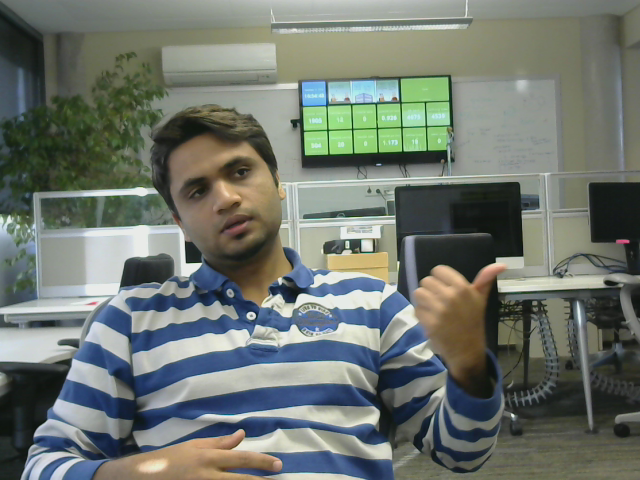
\includegraphics[width=\textwidth]{New_dec/Chet_106.png}
		\caption{}
		\label{}
	\end{subfigure}
	\begin{subfigure}[t]{0.49\textwidth}
		\centering
		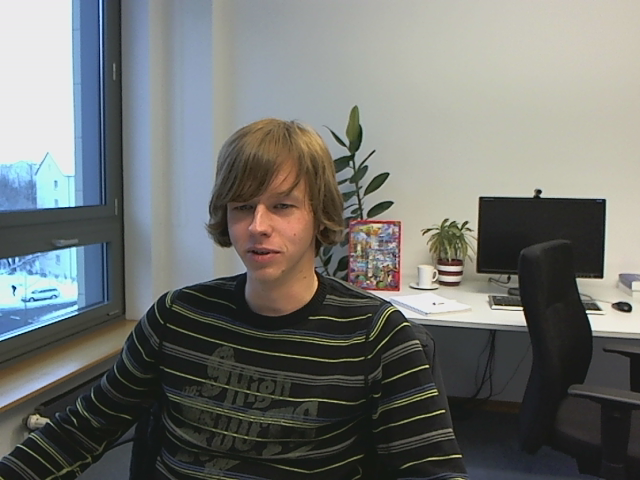
\includegraphics[width=\textwidth]{New_dec/Paul_119.png}
		\caption{}
		\label{fig:PaulDefault120}
	\end{subfigure}
	\begin{subfigure}[t]{0.98\textwidth}
		\centering
		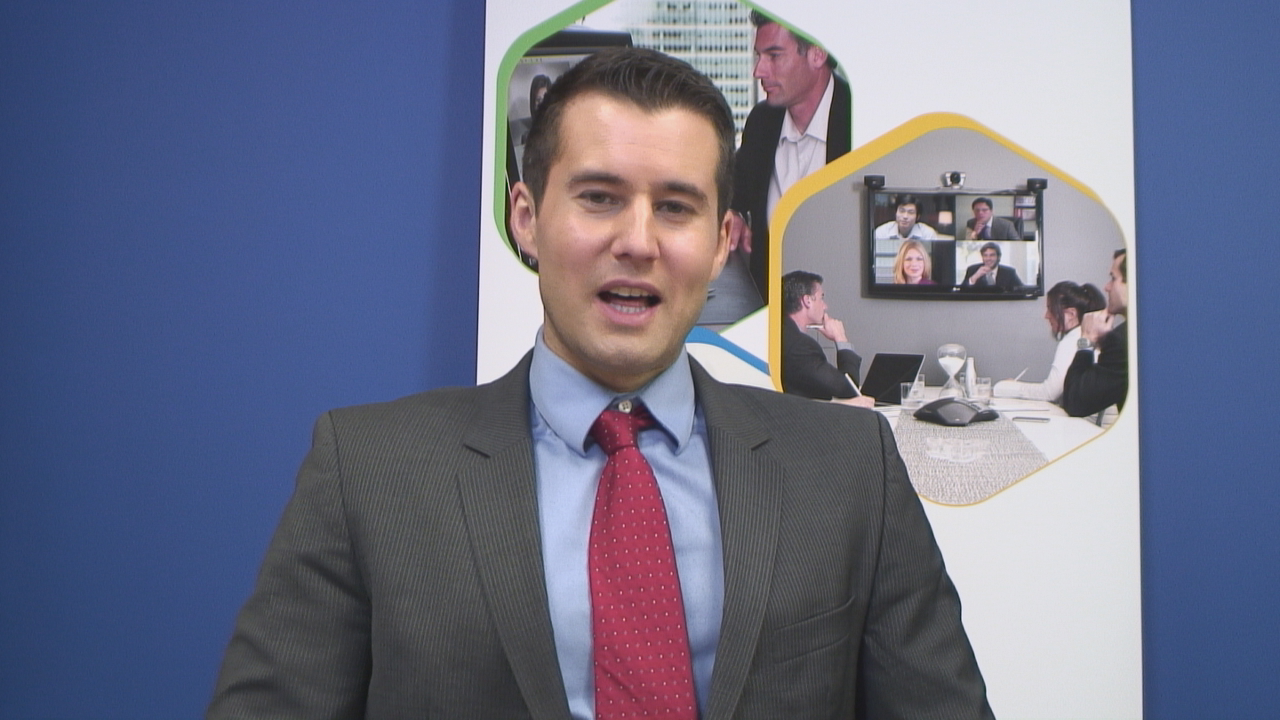
\includegraphics[width=\textwidth]{New_dec/Johnny_35.png}
		\caption{}
		\label{}
	\end{subfigure}
	\caption{Snapshot of test sequence (a)chet640x480, (b)Paul640x480 ,(c)Johnny1280x720.}
	\label{fig:OriginalFrames}
\end{figure}

\section{Encoder Configuration} \label {sec:Encoder configuration}     
This work uses Citrix H.264 video codec for studying different ROI-based encoding approaches. The encoder is configured in low-delay mode suitable for video conferencing and other real-time applications. The bitrate control described in section \ref{chapter:used-bitrate-control-overview} is used to control the output data-rate of the encoder. The encoder is configured to use IPPP mode with key/I-frame used only at the beginning of the sequence followed by only uni-directional P frames. Due to the low-delay requirements there is no provision to re-encode the frame in case of buffer overflow. The frames are dropped entirely in case of a buffer overflow to maintain a constant low-delay.
\begin{table} [!h]
	\centering
	\begin{tabular}{ |c|c|c| }
		\hline
		Name & Bitrate (Kbps) & VBV Size (Bits) \\
		\hline 
		Paul640x480 & 250 & 12500 \\ 
		Chet640x480 & 250 & 12500 \\
		Johny1280x720 & 350 & 17500 \\
		\hline
	\end{tabular}
	\caption{Encoder configuration}
	\label{Table:ConfigurationForEncoding}
\end{table}
The configuration used for encoding each of the sample input sequence listed in the above section is shown in Table \ref{Table:ConfigurationForEncoding}. The bitrates for different input sequence is configured considering the resolution and the complexity of the content. The chosen bitrates are relatively low yielding low visual quality with conventional encoding. This makes it easy to assess the gain in perceptual quality with ROI-based encoding. Figure \ref{fig:ConventionalEncodingFrames} shows the results of conventional encoding for the configuration shown in Table  \ref{Table:ConfigurationForEncoding}. Due to usage of low bitrate, blocky artifacts can be noticed in the face regions.
%Conventional Encoding Images
\begin{figure}[!h]
	\centering
	\begin{subfigure}[t]{0.49\textwidth}
		\centering
		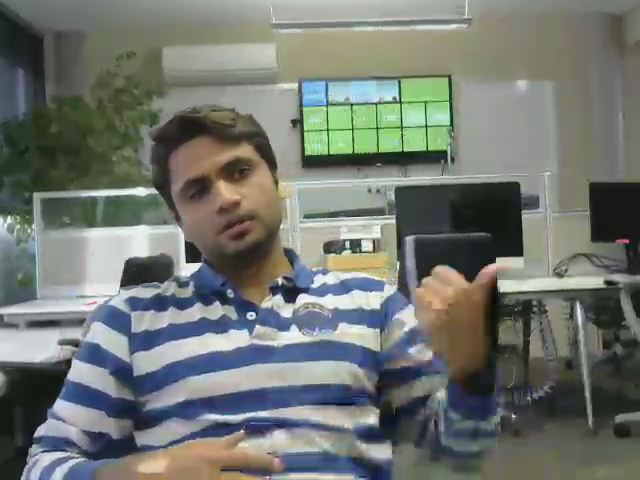
\includegraphics[width=\textwidth]{New_dec/Default/Chet106_250kbpsDefault.png}
		\caption{}
		\label{}
	\end{subfigure}
	\begin{subfigure}[t]{0.49\textwidth}
		\centering
		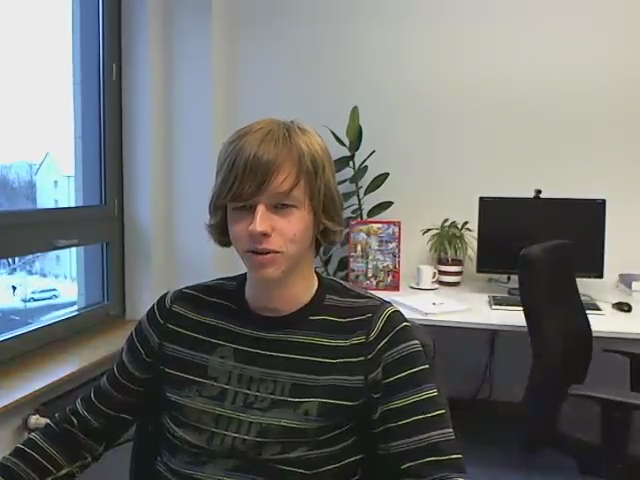
\includegraphics[width=\textwidth]{New_dec/Default/PaulDefault250kbps.png}
		\caption{}
		\label{}
	\end{subfigure}
	\begin{subfigure}[t]{0.98\textwidth}
		\centering
		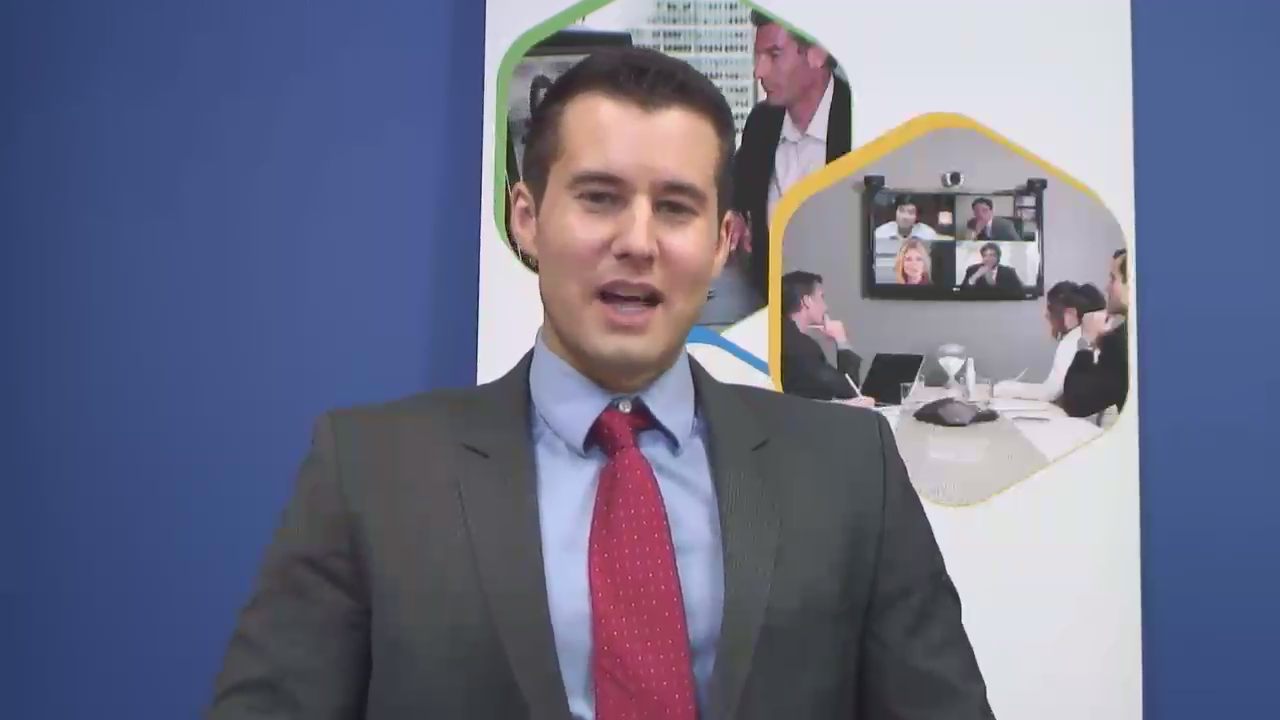
\includegraphics[width=\textwidth]{New_dec/Default/Johnny350kbpsDefault.png}
		\caption{}
		\label{}
	\end{subfigure}
	\caption{Result of Conventional Encoding (a)chet640x480, (b)Paul640x480 ,(c)Johnny1280x720.}
	\label{fig:ConventionalEncodingFrames}
\end{figure}

%\begin{figure}[!h]
%	\centering
%	%Raw YUV image
%	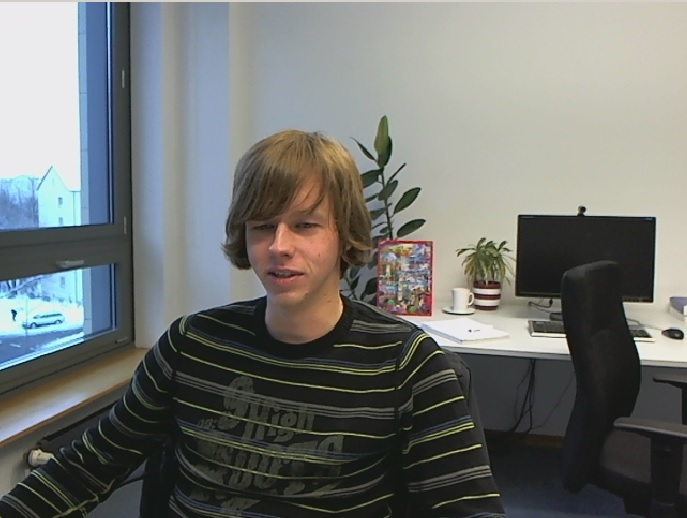
\includegraphics[scale=0.5]{PaulDefault120}
%	\caption{A Frame in the input video}
%	\label{fig:PaulDefault120}
%	%%encoded frame image
%	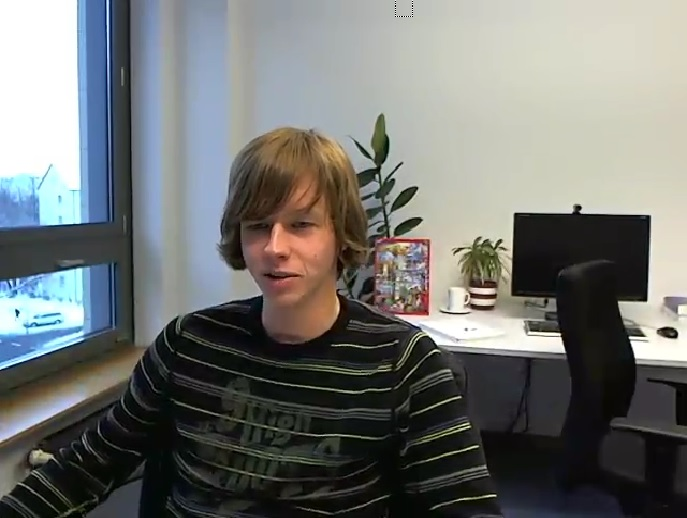
\includegraphics[scale=0.5]{PaulDefault120_91250kbps}
%	\caption{Sample frame of fig \ref{fig:PaulDefault120} encoded at 250kbps}
%	\label{fig:PaulDefaultencoded}
%\end{figure} 


\section{Evaluation Criteria}
One of the crucial aspects in this study is the metric used to evaluate various approaches in order to choose the best approach. The goal of this study is to improve the quality of the ROI macroblocks at the cost of degrading the non-ROI macroblocks. Since the whole approach is to measure the gain in perceptual quality, using frame level PSNR alone as a metric could be misleading. 

In this study, the difference in average PSNR of frames and average ROI PSNR is used as one of the metrics to evaluate different approaches. The expectation is to see an improvement in ROI PSNR, with degradation in PSNR of the non-ROI regions. The shift in quality of ROI and non-ROI parts should be achieved keeping the bitrate unchanged. Therefore, the second aspect is to measure the deviation in bitrate behavior with ROI-based encoding compared to conventional encoding without using any ROI information. Third aspect involves analysis of PSNR and QP variation within a frame. The QP and PSNR distributions within a frame are studied to ensure that there is visible improvement in the quality of ROI without badly degrading the quality of the non-ROI. 

To measure all these behaviors the following metrics are considered. These are discussed in detail in the following sections.
\begin{itemize}  
	\item Quality metrics - PSNR of ROI and non-ROI regions.
	\item PSNR and QP maps - The map of variation of QP and PSNR within a frame.
	\item Delay plot - Plots time delay for every frame.
\end{itemize}

\subsection{Quality Metrics} \label{sec:setup-PSNR}
The increased bit-allocation to ROI macroblocks in ROI-based encoding results in increase in PSNR of the ROI part. This also results in a drop in non-ROI PSNR. Finding the desirable magnitude of improvement in PSNR of ROI along with acceptable drop in PSNR of the non-ROI is tricky. The idea here is to find the right balance between quality improvement in the ROI and the degradation of non-ROI as to achieve maximum perceptual quality. The PSNR computed specific to regions within a frame gives insight into magnitude of transfer of bits from ROI to non-ROI during ROI-based encoding. This measure will also indicate the aggressiveness of an algorithm which is measured in terms of magnitude of objective quality difference forced between ROI and non-ROI parts.

The values in Table \ref{InitPSNR1} show the PSNR values for the conventional video coding for the sample inputs listed in section \ref{sec:sampleInput}. It is clear that for most of the sample inputs, the PSNR of ROI is much lower compared to that of the overall frame PSNR. This is not desirable since the regions that matter the most to the perceptual quality have a lower PSNR on an average.

%Conventional Encoding results
\begin{table} [h!]
	\centering
	\begin{tabular}{ |c|c|c|c| }
		\hline
		Content & PSNR Avg (dB) & PSNR ROI(dB) & PSNR non-ROI(dB) \\
		\hline 
		Paul640x480, 250kbps & 39.15 & 37.72 & 39.22\\ 
		Chet640x480, 250kbps & 31.35 & 32.91 &  31.24\\
		Johny1280x720 350kbps & 37.93 & 36.08 & 38.13\\  
		\hline
	\end{tabular}
	\caption{PSNR values for conventional encoding}
	\label{InitPSNR1}
\end{table}

The PSNR is calculated using the weighted sum of PSNR of individual components per picture (PSNR\textsubscript{Y}, PSNR\textsubscript{U} and PSNR\textsubscript{V}) \cite{ComparingCodingEfficiency}.
\begin{equation}
\label{Eq:PSNR}
PSNR\textsubscript{YUV} = ( 6 \times PSNR\textsubscript{Y} + PSNR\textsubscript{U} + PSNR\textsubscript{V}) / 8,
\end{equation}
where, individual components are computed as,
\begin{equation}
\label{Eq:PSNRDef}
PSNR = 10 \times log_{10}((2^B - 1)^2 / MSE),
\end{equation}

where B = 8 is the number of bits per sample (bit-depth) of the video and MSE is the mean squared error.

The change in PSNR of the ROI and non-ROI parts is measured as an average of PSNR of the entire frame and average of PSNR of ROI of all the frames in the sequence. The PSNR for the entire video sequence can be computed in two ways.
\begin{itemize}
	\item Average of frame PSNR - This is the average of PSNR of all the frames in the sequence.
	\item Average MSE-based PSNR - The PSNR of average MSE of all the frames in the sequence. This is computed by accumulating MSE over entire sequence and then computing PSNR.
\end{itemize}
 The average of PSNR metric is preferred over average MSE based PSNR since the latter metric was found to be heavily influenced by the outliers. For instance, when the sequence has very few extremely low-quality frames but has good quality on an average, the average MSE based PSNR was found to be very low due to presence of very few extremely low-quality frames.

\subsection{PSNR and QP Maps}
The study of PSNR and QP distribution within a frame is important to understand the effect of movement of bits from ROI to non-ROI parts. The PSNR and QP is extracted at the macroblock level. It is then stored in raster scan order which can be used to display as  an image to compare the structure with that of the video frame. These values are illustrated in a gray scale image. 

In a QP scale map, the darker regions in a frame indicate higher quantization. Even though the quantization parameter used for encoding a block is closely related to the PSNR of the block, it is not the only determinative factor. The PSNR can also vary depending on the content. Generally, the lower frequency regions have better PSNR even when encoded with a higher QP. The static regions of the frame also tend to have better PSNR even when higher QP is used because of less new information to be encoded. The PSNR map helps in visualizing the effect of movement of bits from non-ROI to ROI parts.

%The image in Figure \ref{fig:PaulDefault120} shows a frame in the sample video conferencing content with resolution of 640x480 pixels and 30 frames per second. The image in Figure \ref{fig:PaulDefaultencoded} shows the same frame when encoded with the codec configurations discussed in the previous section. The reason for considering a low bitrate of 250 kbps is that it will help in making the improvement in face region and decrease in quality of background more evident and hence will be useful in evaluating different algorithms. 
%Conventional Encoding Images - Quant Maps and PSNR Maps
\begin{figure}[h!]
	\centering
	\begin{subfigure}[t]{0.49\textwidth}
		\centering
		
\includegraphics[width=\textwidth]{New_dec/Default/Chet106_250kbpsDefaultQuant.png}
		\caption{}
		\label{}
	\end{subfigure}
	\begin{subfigure}[t]{0.49\textwidth}
		\centering
		
\includegraphics[width=\textwidth]{New_dec/Default/PaulDefault250kbpsQuant.png}
		\caption{}
		\label{}
	\end{subfigure}
	\begin{subfigure}[t]{0.98\textwidth}
		\centering
		
\includegraphics[width=\textwidth]{New_dec/Default/Johnny350kbpsDefaultQuant.png}
		\caption{}
		\label{}
	\end{subfigure}
	\caption{Quantization maps for conventional encoding (a)chet640x480, (b)Paul640x480 ,(c)Johnny1280x720.}
	\label{fig:OriginalFramesQuantMaps}
\end{figure}

\begin{figure}[h!]
	\centering
	\begin{subfigure}[t]{0.49\textwidth}
		\centering
		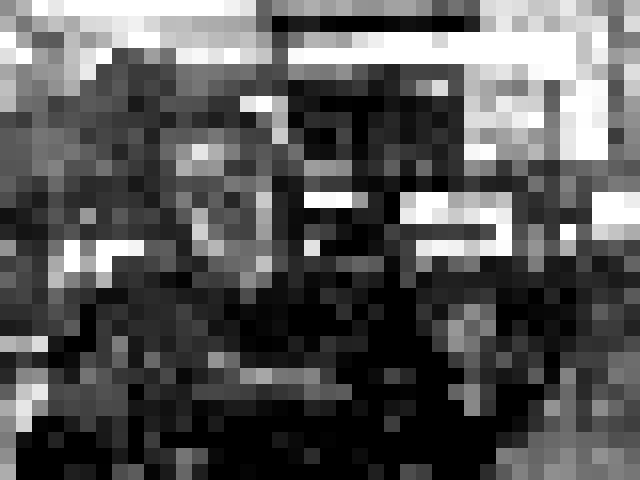
\includegraphics[width=\textwidth]{New_dec/Default/Chet106_250kbpsDefaultPsnrAbs.png}
		\caption{}
		\label{}
	\end{subfigure}
	\begin{subfigure}[t]{0.49\textwidth}
		\centering
		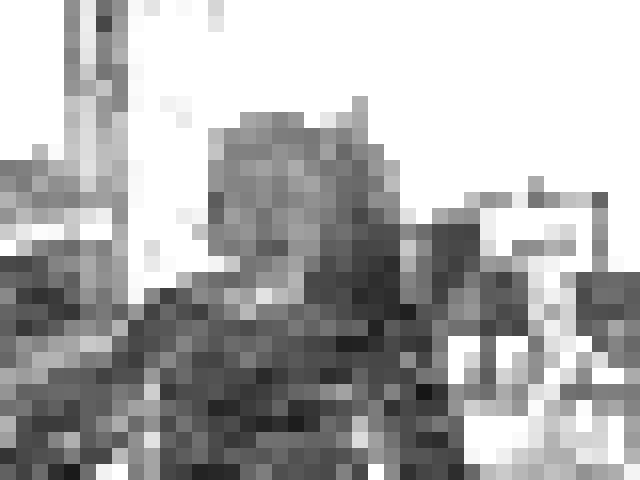
\includegraphics[width=\textwidth]{New_dec/Default/PaulDefault250kbpsPsnrAbs.png}
		\caption{}
		\label{}
	\end{subfigure}
	\begin{subfigure}[t]{0.98\textwidth}
		\centering
		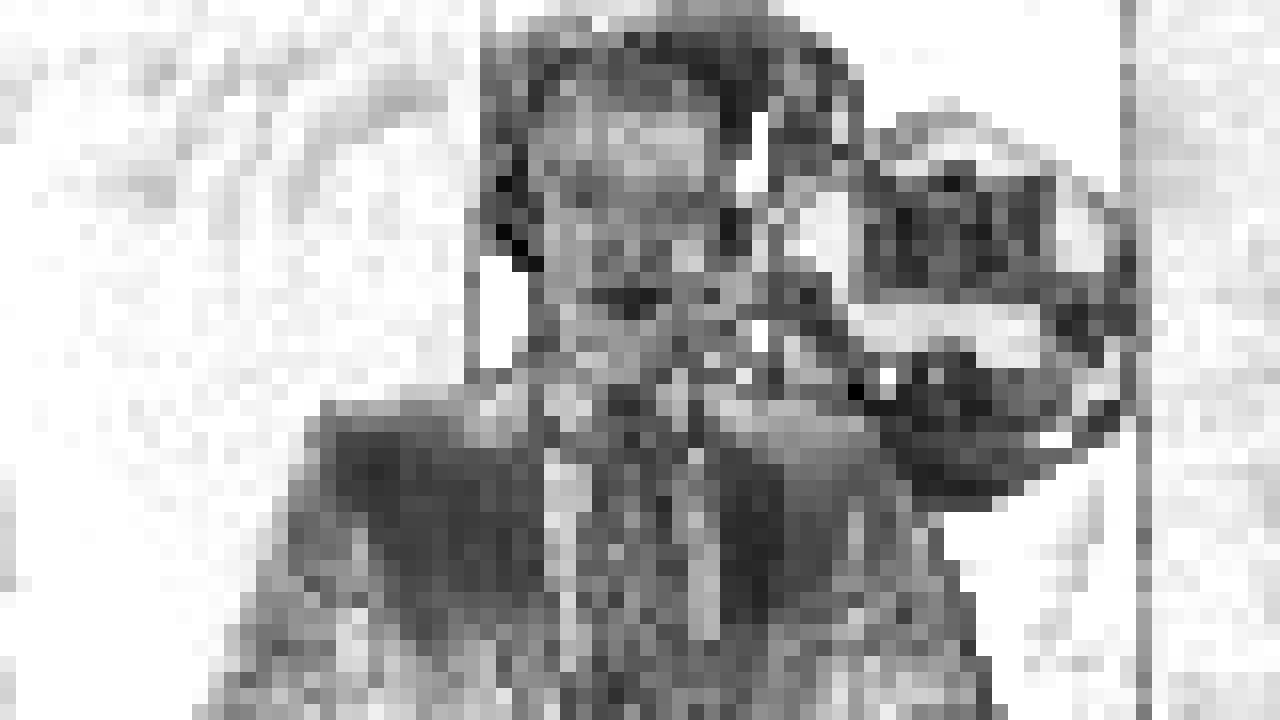
\includegraphics[width=\textwidth]{New_dec/Default/Johnny350kbpsDefaultPsnrAbs.png}
		\caption{}
		\label{}
	\end{subfigure}
	\caption{PSNR maps for conventional encoding (a)chet640x480, (b)Paul640x480 ,(c)Johnny1280x720.}
	\label{fig:OriginalFramesPSNRMaps}
\end{figure}


%\begin{figure}[!h]
%	\centering
%	
\includegraphics[scale=0.5]{PaulDefault120_91250kbps_quant}
%	\caption{Quantization map}
%	\label{fig:PaulDefault120Quant}
%	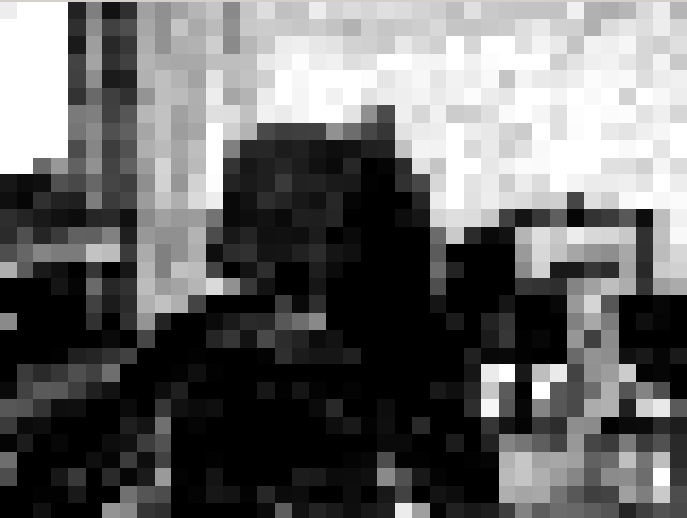
\includegraphics[scale=0.5]{PaulDefault120_91250kbps_psnr}
%	\caption{Relative PSNR map}
%	\label{fig:PaulDefault120PSNR}
%\end{figure} 


The images in Figure \ref{fig:OriginalFramesQuantMaps} shows the quantization parameters used during conventional encoding for the frames in Figure \ref{fig:ConventionalEncodingFrames}. A darker shade of gray in this map indicate usage of higher quantization parameter compared to the regions with brighter shade of gray. The QP range of 1-51 is mapped to gray scale value between 0-255 in the quant maps. It can be noticed that since no information about region of interest is used while encoding the frame, the pattern of quantization appears almost random. The shape of the original content is not recognizable from the quantization map.

The images in Figure \ref{fig:OriginalFramesPSNRMaps} shows the PSNR distribution for the frames in Figure \ref{fig:ConventionalEncodingFrames} which are encoded using conventional encoding. Similar to the quantization map, a brighter shade of gray represents the regions with higher PSNR, the darker regions indicate lower PSNR and worse quality. A PSNR range between 25dB-45dB is linearly mapped to gray scale value of 0-255 in the PSNR maps.
%This map is relative within the frame and does not represent  absolute quality. This map is generated by considering the full range of PSNR of the image after removal of outliers. The map is generated by mapping the PSNR range between 10th percentile and 90th percentile of the whole frame to values between 0 to 255.

It is evident that the structure of the original content is preserved in the PSNR map. In most of the contents (Johnny1280x720 and Paul640x480), the background regions have better PSNR, the foreground has worse quality and the difference in quality is quite huge. The difference in the quality is due to the fact that background in a video conferencing scenario is mostly static and hence gets encoded better with every frame. On the other hand, the foreground has motion and new data to be encoded, hence it cannot achieve the same quality as the background. Since the focus of attention during video telephony is foreground or the face region, improving the face region must help in improving overall perceptual quality. The PSNR maps help to visualize the effect of such preferential encoding. The goal of ROI-based encoding is to reduce the PSNR difference between foreground and background and to boost the quality of the foreground(face regions) to same level as the background or even better.

%%
%%Bitrate Fluctuation and delay plots
%%
\subsection{Delay Plot} \label{sec: setup delay plots}
The fundamental idea in this work is to efficiently use the bits within a frame to encode the region of interest with better quality. The algorithms used to achieve this should not alter the behavior of the encoder in terms of frame level bit-consumption. As mentioned in previous sections, in case of VBV overflow, the encoder drops the frame in order to maintain strict VBV compliance. The dropped frames result in jerky playback and hence should be avoided. The ROI-based bitrate control scheme should not contribute to an increase in the number of dropped frames due to changes in the bit-consumption pattern.

In contant bitrate control, the size of an encoded frame decides the buffering delay of each frame. Therefore, any change in bit-consumption pattern at the frame level gets reflected in the buffering delay of corresponding frames. The delay due to buffering of each frame in the sequence is plotted to analyze the bit-consumption behavior. Figure \ref{fig:ConventioanlEncodingDelay} is the delay plot of the sample video sequences encoded with the configuration shown in Table \ref{Table:ConfigurationForEncoding}. Every point in the delay plot specifies the time taken by the corresponding frame (marked on the x-axis) to reach the decoder assuming zero transmission delay. It can be noticed the delay is almost constant for Johnny1280x720 and Paul640x480. However, there is slight variation for chet640x480 due to high temporal complexity.

The curve in delay plots appear mostly smooth except for few sudden drops (zero values). These zero-valued points indicate dropped frames. Since these frames are not included in the final bitstream and hence not transmitted, the delay is indicated as zero. Ideally, The ROI-based encoding approaches should not alter the shape of this plot. The ROI-based bitrate control should re-distribute the bits within a frame with minimum error carried to the next frame. It is also not desirable to have any increase in the number of dropped frames.
\begin{figure}[h!]
	\centering
	\begin{subfigure}[t]{0.49\textwidth}
		\centering
		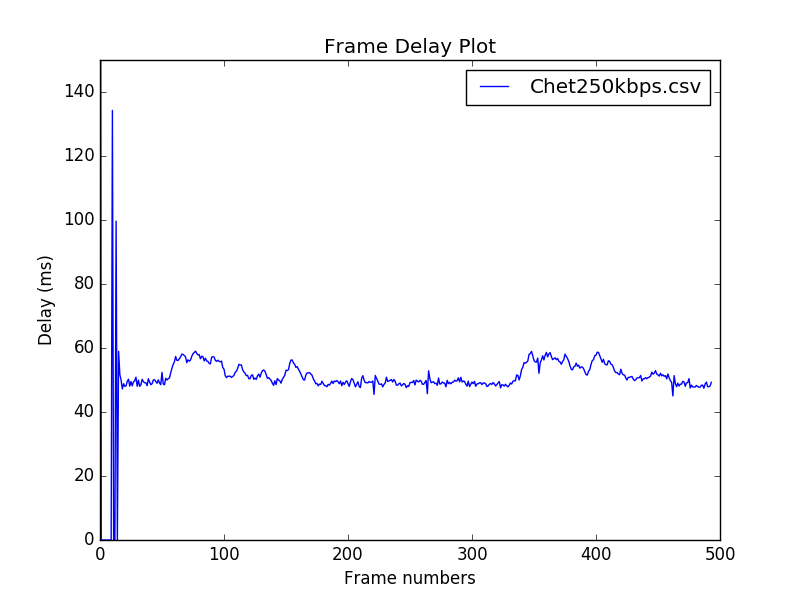
\includegraphics[width=\textwidth]{New_dec/Default/Chet250kbpsDefaultDelay.png}
		\caption{}
		\label{}
	\end{subfigure}
	\begin{subfigure}[t]{0.49\textwidth}
		\centering
		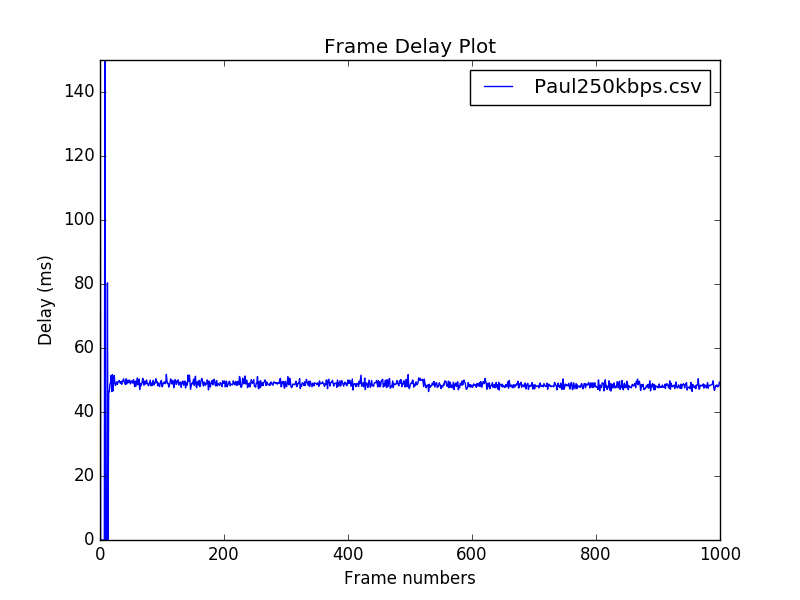
\includegraphics[width=\textwidth]{New_dec/Default/PaulDefault250kbpsDelay.png}
		\caption{}
		\label{}
	\end{subfigure}
	\begin{subfigure}[t]{0.49\textwidth}
		\centering
		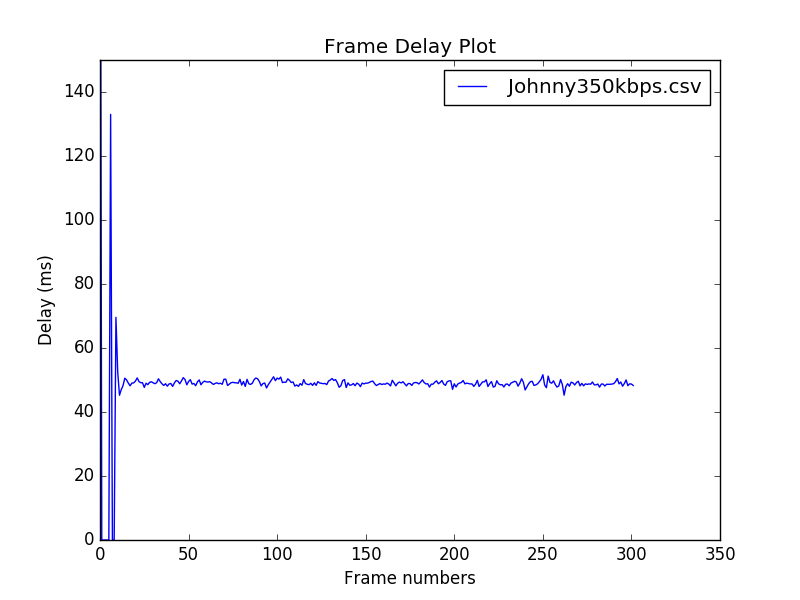
\includegraphics[width=\textwidth]{New_dec/Default/Johnny350kbpsDefaultDelay.png}
		\caption{}
		\label{}
	\end{subfigure}
	\caption{Delay plot for conventional encoding (a)chet640x480, (b)Paul640x480 ,(c)Johnny1280x720.}
	\label{fig:ConventioanlEncodingDelay}
\end{figure}

%\begin{figure}[!h]
%	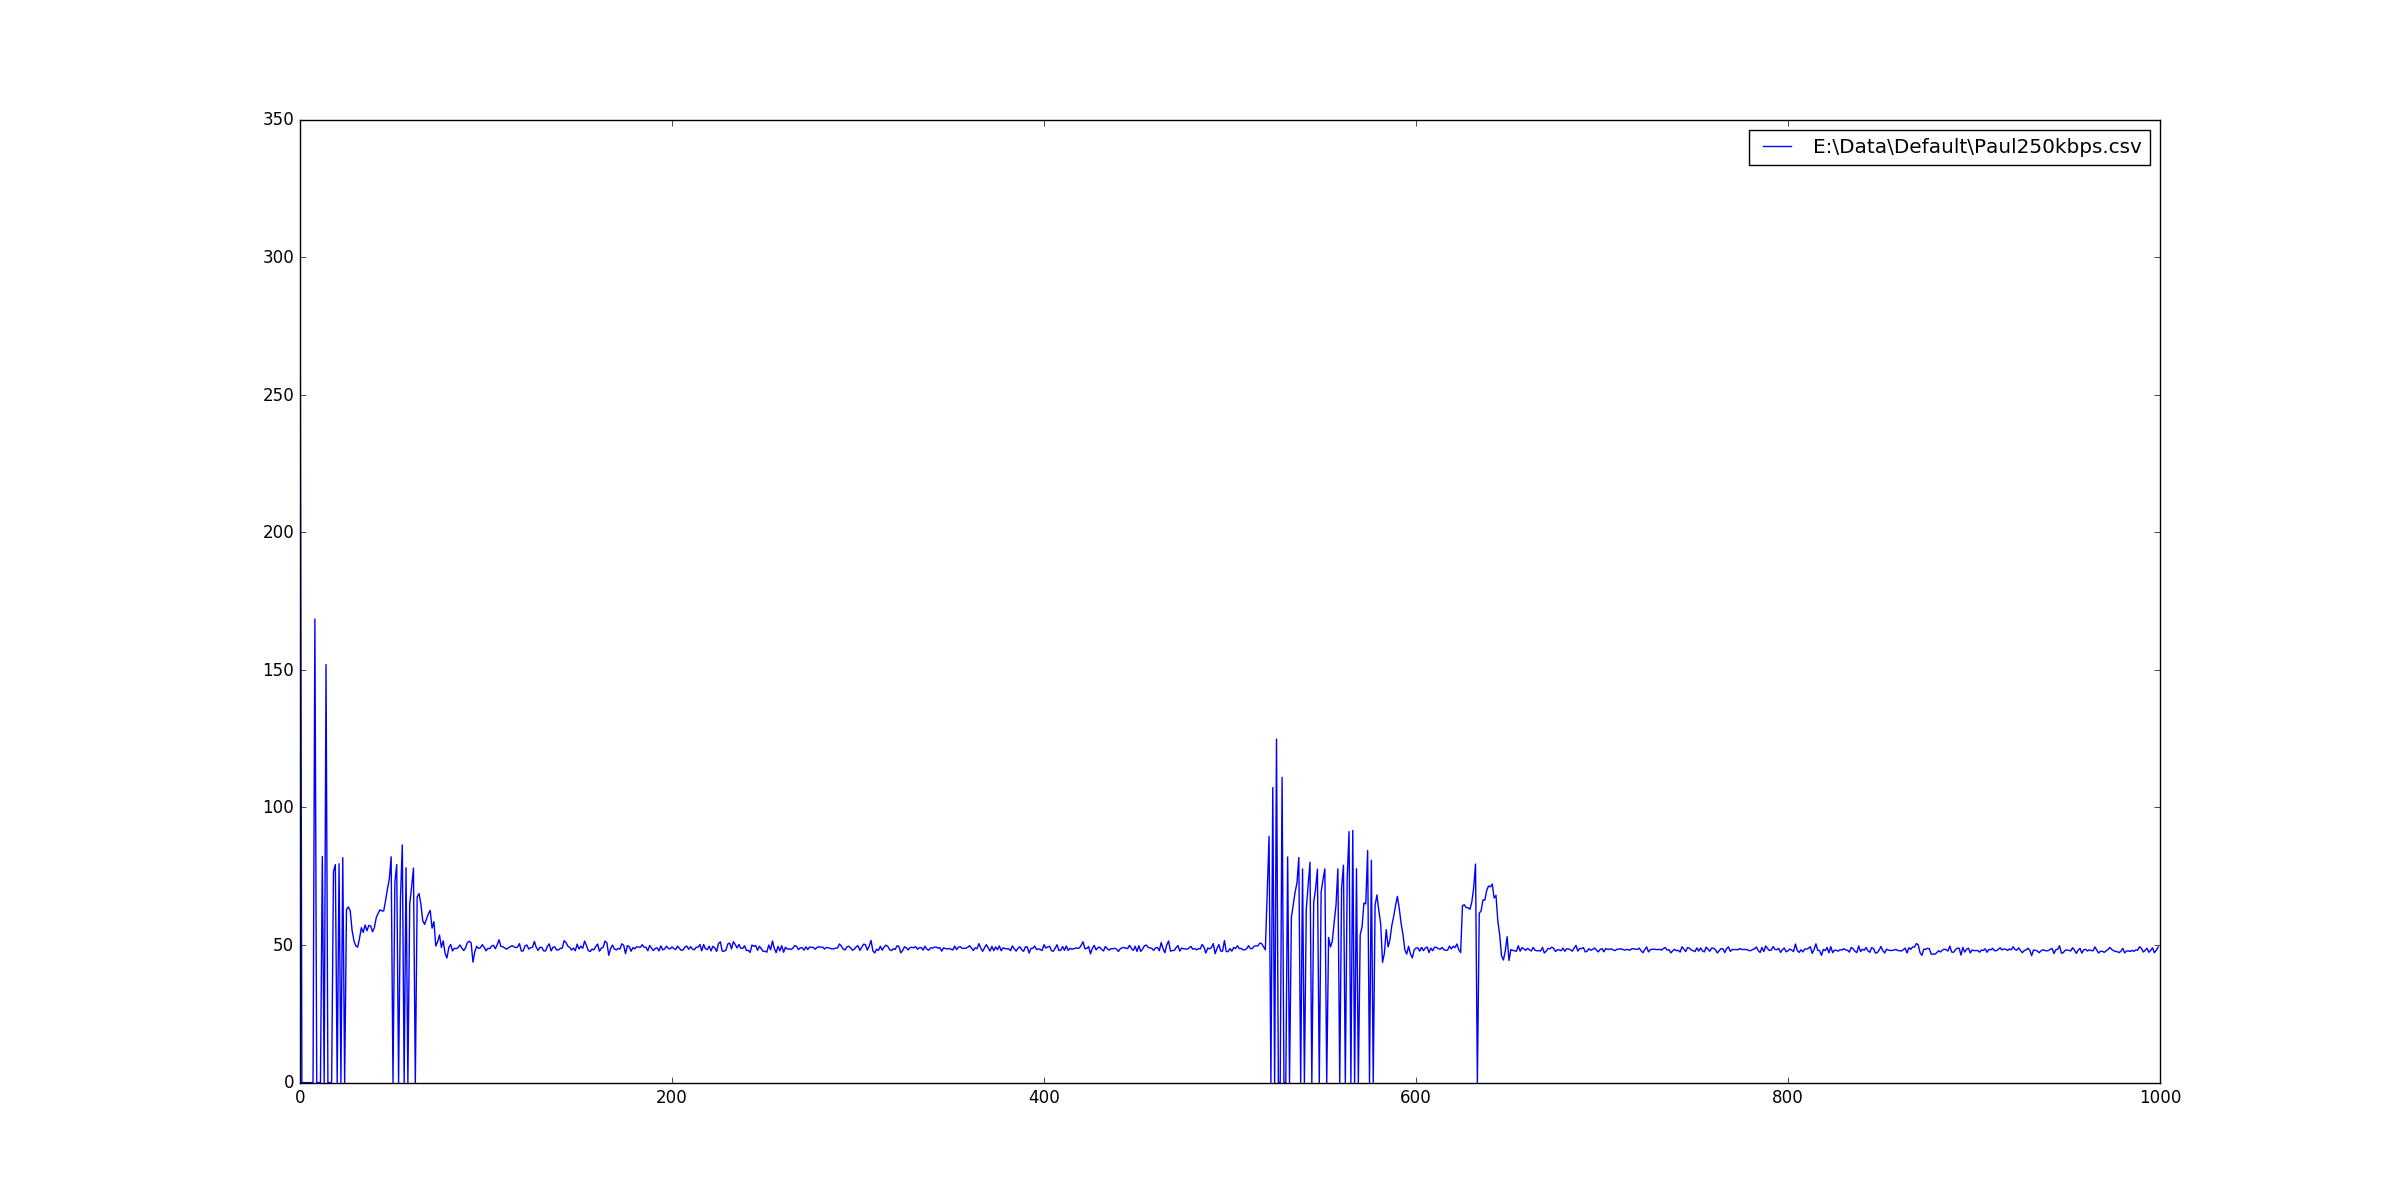
\includegraphics[scale=0.25]{PaulDefault250kbpsDelay}
%	\caption{Delay plot}
%	\label{fig:PaulDefault250kbpsDelay}
%\end{figure} 

%Face Detection
%Face Detection
%
\chapter{Face Detection and Tracking}
\thispagestyle{empty}% no page number in chapter title page
In video conferencing, face is the most important region in the video stream to the viewer. In this work, various approaches of improving perceptual quality by increasing quality of the face region are presented. The prerequisite for these ROI-based encoding techniques is precise co-ordinates of the face (ROI) in any given video frame. This section describes the setup used to detect face prior to encoding.

The face detection module is independent of the encoder and ROI-based encoding schemes discussed in this work. The face detection module uses input video stream to the encoder and marks the ROI at the macro block level. Figure \ref{fig:PaulDefault120FaceMap} shows the face map generated for the frame shown in Figure \ref{fig:PaulDefault120}. Each byte value in the face-map generated by face detection module represents a macroblock scanned in raster scan order. A value of 0xff signifies macroblock being part of the face or ROI and 0x00 represents a normal macroblock.  The region in white is considered as ROI. This information is used by the bitrate control module of the encoder for ROI-based encoding.

Since every ROI-based encoding approach discussed in this work involves improving the ROI at the cost of degrading the quality in non-ROI, it is very important to have high reliability with face detection. Any false detection will lead to degradation of the actual ROI compared to conventional encoding. Therefore, the damage caused by a false detection is higher than the loss due to not detecting any face.
\begin{figure}[h!]
	\centering
	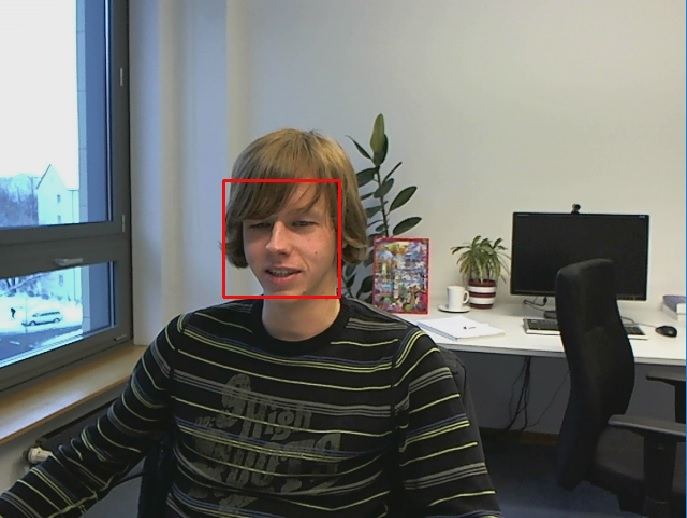
\includegraphics[scale=0.4]{PaulDefault120FaceRecognized}
	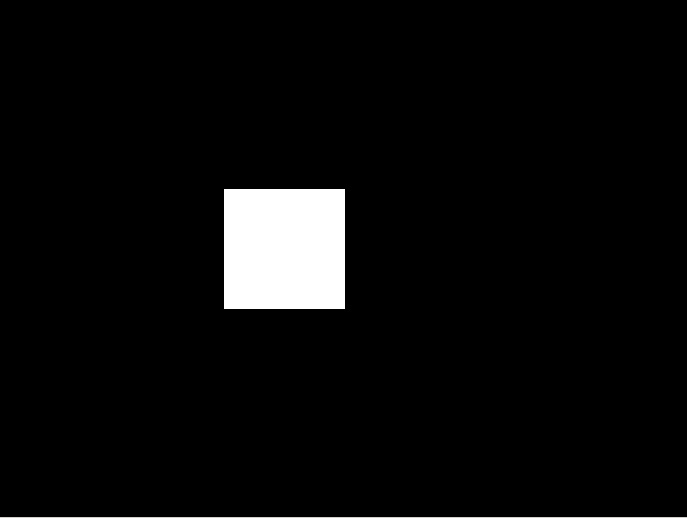
\includegraphics[scale=0.4]{PaulDefault120FaceMap}
	\caption{Face Detection binary map}
	\label{fig:PaulDefault120FaceMap}
\end{figure}

\section{Viola Jones Face Detection}
Many open-source solutions like OpenCV offers a ready to use solution that can be integrated with the codec library. In this work, OpenCV implementation of Viola-Jones face detection algorithm \cite{Viola01rapidobject} is used. It has large set of trained classifiers considering many types of faces and viewing angles. A standard frontal face haar-classifier was used to detect faces in all the sample video sequence.

\subsection{Performance Benchmark}
In this work, face is detected independently in every frame of the video stream. This is used to achieve high accuracy face detection to evaluate ROI-based encoding techniques. This setup is not the most optimal solution to be used in a real-time system. Face detection is a computation intensive task and performing this task on every frame of the video stream demands huge computation power. \Cref{Table:FaceDetectionBenchMark} shows the measured performance of OpenCV based face detection on Intel(R) Xeon(R) CPU E3-1225 V2 @ 3.20 Ghz. The numbers mentioned in \Cref{Table:FaceDetectionBenchMark} also account for input raw file format conversion in addition to face detection. It is clear that the face-detection module complexity increases almost linearly with resolution. For a resolution of 1280x720, the processing is not real-time (assuming 30fps video stream) with specified computation resource. Following section proposes optimization scheme to detect the face in real-time.
\begin{table} [h!]
	\centering
	\begin{tabular}{ |c|c|c| }
		\hline
		Name & Resolution & Frames Per Second \\
		\hline 
		Paul640x480 & 640x480 & 44.26 \\ 
		Johny1280x720 & 1280x720 & 18.89 \\
		\hline
	\end{tabular}
	\caption{OpenCV face detection performance benchmark}
	\label{Table:FaceDetectionBenchMark}
\end{table}

\section{Optimization Using Motion Vectors}
As mentioned above, it is not an optimal solution to invoke face detection module for every frame of the input video stream. Usually, face tracking techniques are used to track the face once it is detected. Some of the conventional approaches for tracking are mean-shift and continuous adaptive mean shift (CAMSHIFT) \cite{CAM-shift}. However, these techniques also demand considerable amount of computation resource and requires additional effort to implement face tracking in addition to face detection.

\subsection{Regular Interval Face Detection}
An alternate approach is to detect face at regular intervals in every $nth$ frame instead of every frame. Due to high frame-rate of the input video stream, the movement of face region is limited between the consecutive frames. The intermediate frames consider the previously detected face region as face. In other words, the approach is to use the temporally subsampled video stream with sampling interval $n$ as input to the face detection module. However, this approach of temporally subsampled face detection leads to inaccuracy which increases with sampling interval between two frames in which face is detected. The inaccuracy also increases with rapid movements in face regions. 

\Cref{fig:FDnFrameWorstError} shows a snapshot of the sample input content vidyo1280x720 with 30 frames per second with face detection at every frame and at regular intervals (temporal sub-sampling). The green bounding box represents output with face detection on every frame ($n=1$) and the red bounding box represents face detection performed on every 15th frame ($n=15$). It is clear that there is a large inaccuracy with temporally subsampled face detection. For sampling interval $n=15$, majority of the face region lies outside the bounding box. This can degrade the performance of ROI-based encoding since the region most important to perceptual quality is considered as non-ROI. The error due to temporal subsampling is measured as the euclidean distance (pixels) between the top-left corner pixels of two bounding boxes. The error is always computed with respect to the green bounding box ($n=1$). \Cref{Table:FaceDetectionError} shows the error with different sampling intervals for face detection.

\begin{figure}[h!]
	\centering
	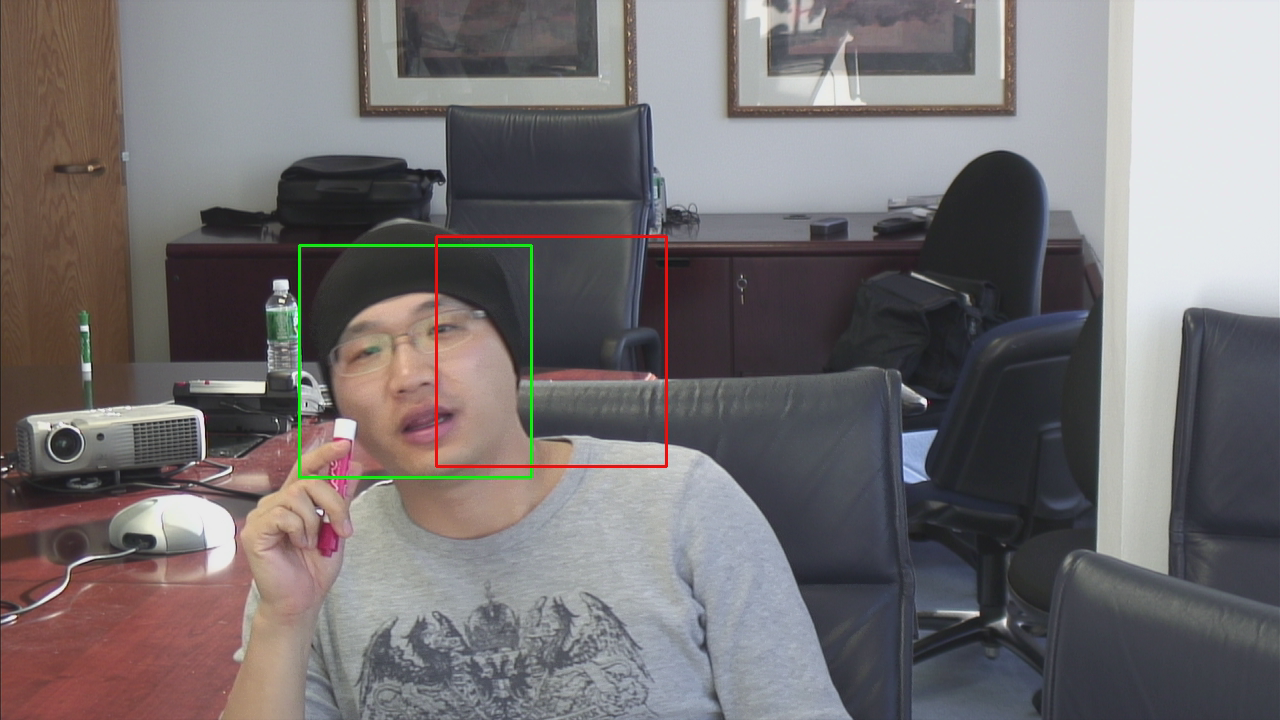
\includegraphics[scale=0.4]{FaceTracking/everyNframe/vidyo4_180_worstcaseerror.png}
	\caption{Snapshot of vidyo1280x720 with face detection at regular interval (temporal sub-sampling). Green and red bounding box represents face detection at every frame and every 15th frame respectively.}
	\label{fig:FDnFrameWorstError}
\end{figure}

\begin{table} [h!]
	\centering
	\begin{tabularx}{0.9\linewidth}{ |Y|Y|Y| }
		\hline
		\textbf{Sampling interval for face detection(n)} & \textbf{Average error(pixels)} & \textbf{Maximum error(pixels)} \\
		\hline 
		5 & 8.06 & 57.55 \\ 
		10 & 16.89 & 112.21 \\
		15 & 23.27 & 137.29 \\
		\hline
	\end{tabularx}
	\caption{Inaccuracy due to face detection at regular intervals ($n$)}
	\label{Table:FaceDetectionError}
\end{table}

During video conference, face region is mostly static except for movement of lips and eye regions. The face detection at regular intervals is not an optimal solution due to the following reasons.
\begin{itemize}
	\item The face detection module is invoked even when the face region is static. This is wastage of precious computation resource.
	\item The error during sharp movements in face region is very high as shown in \Cref{Table:FaceDetectionError}.
\end{itemize} 

In order to address the above disadvantages, this work proposes an alternative approach in which motion vector information computed during motion estimation stage of video encoding is reused to detect the movement of face to invoke face detection instead of detecting face in every $nth$ frame.

\subsection{Face movement and motion vector}
\begin{figure}[h!]
	\centering
	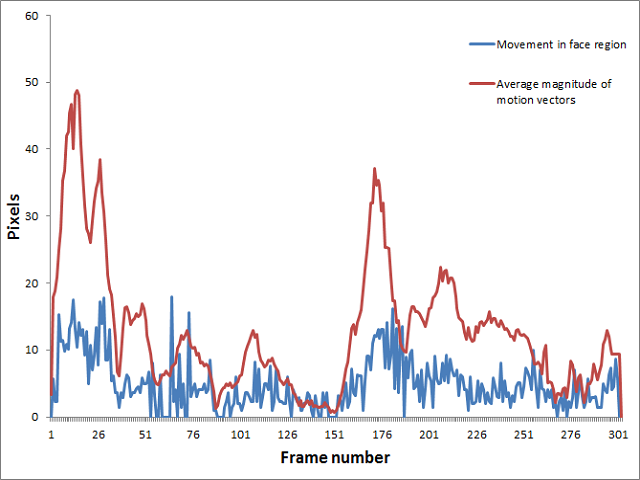
\includegraphics[scale=0.8]{FaceTracking/MotionVSMotionVectorVidyo4.png}
	\caption{Comparison of movement of face region between consecutive frames(blue) and average magnitude of motion vectors in the face region(red).}
	\label{fig:MotionVSMotionVector}
\end{figure}
Any movement in face region is reflected in the motion vectors of macroblocks in the corresponding regions. The magnitude of these motion vectors is directly proportional to the magnitude of movement in the face region. \Cref{fig:MotionVSMotionVector} shows the predictability of sharp movements in face regions with average magnitude of motion vectors of face regions. The series in blue represents the difference between top-left corner pixels of bounding boxes of detected face in a given frame and its previous frame. The face detection is performed on every frame of the video stream ($n=1$). The series in red represents the average magnitude of motion vectors in face region of any given frame predicted from its previous frame. It is clear that all sharp movements in the face region have corresponding high magnitude motion vectors. This shows that sharp movements in face region is easily predictable from the motion vectors of corresponding regions.

\subsection{Motion Vector Based Variable Interval Face Detection}
The predictability of sharp movements of face region using motion vectors can be used to find the optimal interval to perform face detection. The  idea is to perform face detection when sharp movement in face region is detected using motion vectors. This does not alter the face detection or tracking algorithm used, but it invokes these modules only when the movement in the face region is detected. The algorithm used to perform variable interval face detection based on motion vector is as follows.
\begin{enumerate}
	\item Perform face detection on the first frame.
	\item Consider the previously detected face region as face in the subsequent frames until face detection is performed again.
	\item For every frame, compute the average magnitude of motion vectors of all the macroblocks belonging to the face region. If the average magnitude is greater than a predetermined threshold ($T_H$), perform face detection on the current frame.
	\item It is possible that face region can slowly drift with average motion vector less than $T_H$ on every frame. To correct accumulated error due to such gradual motion of face region, face detection is performed after large number of frames ($N$) even if no motion is detected. Since the movement of face region is very slow in this case, a large sampling interval $N$ can be used such that $N >> n$ . 
\end{enumerate}
\begin{figure}[h!]
	\centering
	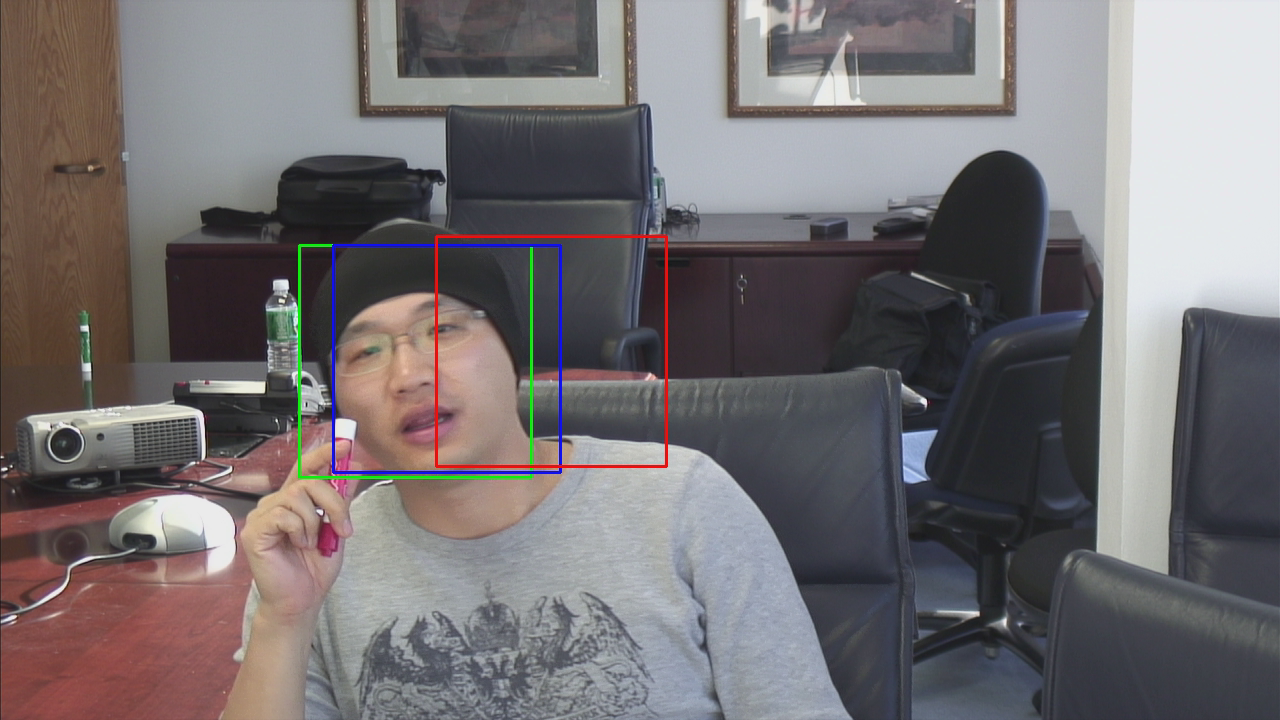
\includegraphics[scale=0.4]{FaceTracking/motion_vector/vidyo4_180_worstcaseerror.png}
	\caption{Face detection at regular interval shown in \cref{fig:FDnFrameWorstError} along with motion vector based variable interval face detection (blue bounding box).}
	\label{fig:FD_all}
\end{figure}

The technique described above will avoid wastage of computation resource by avoiding face detection or tracking when face region is highly static. This will also reduce the error due to face detection with temporal subsampling since face detection is performed immediately after considerable movement of face region is detected. \Cref{fig:FD_all} shows the same frame shown in \Cref{fig:FDnFrameWorstError} with motion vector based variable interval face detection (shown as blue bounding box). It is clear that the inaccuracy in face detection is much lower compared to the approach where face is detected in every 15th frame ($n=15$). 

The comparison of inaccuracies with regular interval face detection with $n=15$ and motion vector based variable interval face detection is shown in \Cref{Table:FaceDetectionComparison}. The total number of face detection performed in a sequence of 300 frames for both the approach is almost the same. This implies that the computation resource required for face detection with these approaches remain almost the same. The chosen sample content has very high motion in the face region which results in higher number of face detection performed based on the motion vector information. For a typical video conferencing stream, the number of face detection is expected to be much lower compared to regular interval face detection. However, the error due to temporal subsampling is greatly reduced with motion vector based variable interval face detection. The advantages and disadvantages of using motion vector based variable interval face detection instead of regular interval face detection are summarized below.

%Table showing improvement with face detection based on motion vectors
\begin{table} [h!]
	\centering
	\begin{tabularx}{0.9\linewidth}{ |Y|Y|Y|Y| }
		\hline
		\textbf{Face detection interval} & \textbf{Total number of face detection} & \textbf{Average error (pixels)} & \textbf{Maximum error (pixels)}\\
		\hline 
		regular interval, n=15 & 21 & 23.27 & 137.29 \\ 
		\hline
		motion vector based variable interval & 23 & 17.45 & 59.93\\
		\hline
	\end{tabularx}
	\caption{Performance of regular interval and motion vector based variable interval face detection.}
	\label{Table:FaceDetectionComparison}
\end{table} 

\subsection*{Advantages}
\begin{itemize}
	\item The average error due to not performing face detection on every frame is greatly reduced.
	\item The ROI-based encoding techniques are highly sensitive to maximum error in face detection. This is reduced by a factor greater than two since sudden motion always triggers face detection.
	\item For a typical video conferencing stream the total number of face detection performed will be lower compared to regular interval face detection. This reduces the overall computation requirement making it easier to achieve real-time performance. 
	\item This approach is based on reuse of motion vectors computed during video encoding. Therefore it has very low computation complexity.
\end{itemize}
\subsection*{Disadvantages}
\begin{itemize}
	\item Unpredictable load - In motion vector based variable interval face detection, the number of face detection performed for a given sequence depends on the magnitude of motion in the face region. This varies across different contents. Therefore, the processing load due to this approach is not predictable.
	\item Higher peak load - Motion vector based variable interval face detection can trigger too many face detection in a small interval due to very high motion in the face region.
\end{itemize}
%\begin{table} [h!]
%	\centering
%	\begin{tabular}{ |r|r|r|r| }
%		\hline
%		\multirow{2}{*}{\parbox{0.25\linewidth}{Face Detection interval}} & \multirow{2}{*}{\parbox{0.25\linewidth}{Total face detections}} & \multirow{2}{*}{\parbox{0.15\linewidth}{Avg Error (pixels)}} & \multirow{2}{*}{\parbox{0.15\linewidth}{Max Error (pixels)}}\\ 
%		& & & \\ 
%		\hline
%		\multirow{2}{*}{\parbox{0.3\linewidth}{Improved QP Offset based ROI encoding}}  & Paul640x480, 250kbps & 38.29 & 40.10\\ 
%		& Johnny1280x720 350kbps & 37.50 & 37.37\\ 
%		\hline
%		\multirow{2}{*}{\parbox{0.3\linewidth}{ROI-based Bit-allocation}} & Paul640x480, 250kbps & 38.22 & 40.95\\ 
%		& Johnny1280x720 350kbps & 36.94 & 38.57\\  
%		\hline 
%	\end{tabular}
%	\caption{PSNR Comparison for different approaches of ROI encoding}
%	\label{Table:AllPSNR1}
%\end{table}
%Most available face detection algorithms work on the pixel domain. These algorithms provide good level of detection accuracy. The main drawback of this approach is that they are computationally intensive. As discussed earlier, the use case considered in this work has very less room for additional computations. Therefore, in this work ways of compressed domain face detection is explored to detect faces with less computational requirements.

%\subsection{Spatial Domain Face Detection}
%In this approach, the face detection algorithms work directly on the pixel values. This approach is simple in terms of implementation. Many open-source solutions like OpenCV offers a ready to use solution that can be integrated with the codec library. It has large set of trained classifiers considering many types of faces and viewing angles. However, this is a computation intensive approach and almost impractical to use in the final solution. 
%\subsection{Compressed domain Face Detection}
%Most available face detection algorithms work on the pixel domain. These algorithms provide good level of detection accuracy. The main drawback of this approach is that they are computationally intensive. As discussed earlier, the use case considered in this work has very less room for additional computations. Therefore, in this work ways of compressed domain face detection is explored to detect faces with less computational requirements. 

%
%Face Detection
%
%\chapter{Face Detection}
%\thispagestyle{empty}% no page number in chapter title page
%
%Face detection algorithms are used to mark the region of interest in the current frame. All the algorithms considered for intelligent bit allocation involve improving the region of interest at the cost of rest of the frame. Therefore, it is very important to have high reliability with face detection. Any false detection will lead to degradation of the actual region of interest compared to normal encoding, this should be avoided in all scenarios. The damage caused by false detection is higher than the loss due to not detecting any face. Therefore, a high threshold must be used to declare any region of the frame as face.
%
%\begin{figure}[!h]
%	\centering
%	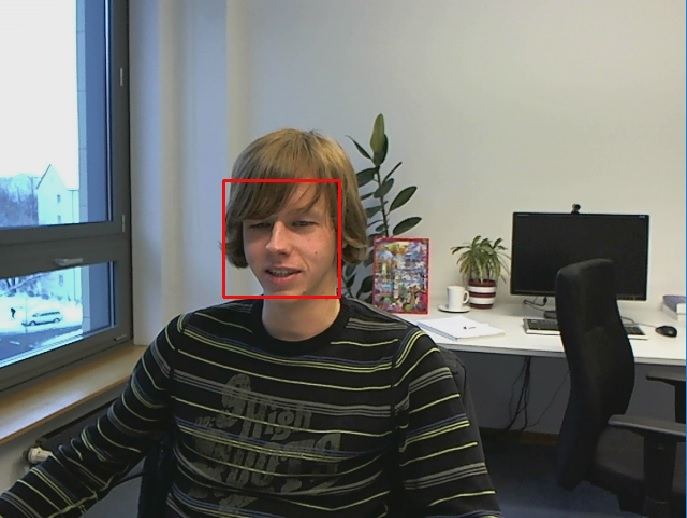
\includegraphics[scale=0.4]{PaulDefault120FaceRecognized}
%	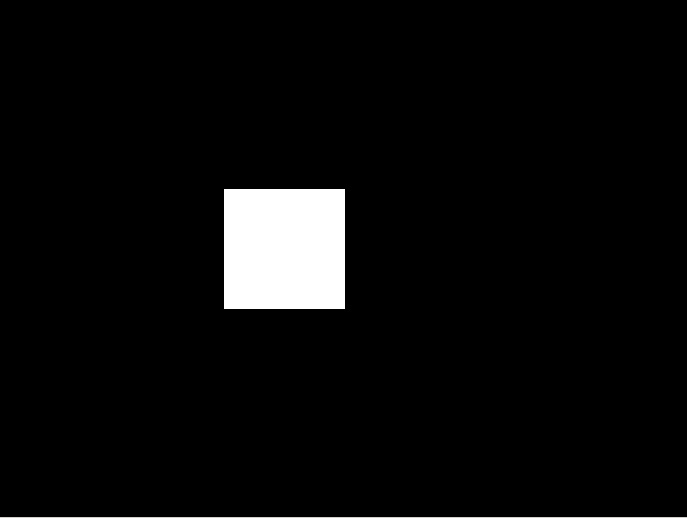
\includegraphics[scale=0.4]{PaulDefault120FaceMap}
%	\caption{Face Detection binary map}
%	\label{fig:PaulDefault120FaceMap}
%\end{figure}
%
%The face detection module itself shall not be a part of the encoder, but the output from the face detection is a binary file with face regions marked is used as input by the encoder. In this work, the face detection module uses input YUV to the encoder and marks the region of interest at the macro block level. Each byte value in the output file of face detection module represents a macro-block scanned in raster scan order. A value of 0xff signifies macro-block being part of the face or region of interest and 0x00 represents a normal macro-block. Figure \ref{fig:PaulDefault120FaceMap} represents the face map generated for the frame shown in Figure \ref{fig:PaulDefault120}. The region in white is considered as region of interest, this information is used inside the bitrate control module of the encoder to perform intelligent bit allocation.
%
%Different approaches are used to detect the face region in the video. There is always a trade-off between accuracy of face detection algorithm and its complexity. The work presented here is mostly relevant to real time systems. Any added complexity due to additional module of face detection will cause significant delay which is totally unacceptable in such systems. Therefore, the algorithm chosen for face detection must be light weight and reasonably accurate in all lighting conditions. 
%
%\section{Spatial Domain Face Detection}
%In this approach, the face detection algorithms work directly on the pixel values. This approach is simple in terms of implementation. Many open-source solutions like OpenCV offers a ready to use solution that can be integrated with the codec library. It has large set of trained classifiers considering many types of faces and viewing angles. However, this is a computation intensive approach and almost impractical to use in the final solution. 
%\section{Compressed domain Face Detection}
%Most available face detection algorithms work on the pixel domain. These algorithms provide good level of detection accuracy. The main drawback of this approach is that they are computationally intensive. As discussed earlier, the use case considered in this work has very less room for additional computations. Therefore, in this work ways of compressed domain face detection is explored to detect faces with less computational requirements. 
%Many works have been published
%TBD LATER
%
%Different approaches
%
% 
\chapter{ROI-based Bitrate Control} \label{chapter:ROI-RC}
\thispagestyle{empty}% no page number in chapter title page

As discussed in the previous sections there are many ways in which ROI information can be used to improve the perceptual quality of the video. This section describes the following two major approaches of ROI-based bitrate control to enhance the quality of the ROI macroblocks. 
\begin{itemize}
	\item ROI QP Offset
	\item ROI-based Bit-Allocation
\end{itemize}
These approaches are designed considering the bitrate control module described in chapter \ref{chapter:used-bitrate-control-overview}. However, the underlying principles of ROI-based encoding to create an optimal quality difference between ROI and non-ROI are applicable to any generic bitrate control modules. The principles presented in this work can be used to modify other standard low-delay bitrate control algorithms to produce equivalent results. The different approaches presented here vary in terms of ease of implementation, complexity and output quality. This offers flexibility to choose a suitable approach according to the specific requirements. The following subsections describe each of the ROI-based bitrate control approaches.

\section{ROI QP Offset}
A simple way of creating a bias in the quality between ROI and non-ROI is by using a QP offset for the macroblocks belonging to the ROI. A negative QP offset ($dq_{roi}$)is added to the QP allocated by the bitrate control module ($Q_m$) for ROI macroblocks. The QP for a macroblock assigned by the bitrate control is modified before using it for the final encoding as shown below.
$$Q_m^{roi} = Q_m - dq_{roi},$$
$$Q_m^{nroi} = Q_m.$$
Where, $Q_m^{roi}$ and $Q_m^{nroi}$ are the QP used for encoding a macroblock belonging to ROI and non-ROI parts respectively. The QP offset is used outside the bitrate control module, hence this approach requires minimum or no modifications to the bitrate control module. 

The effects on encoding of non-ROI macroblocks due to usage of external QP offset for ROI macroblocks are:
\begin{itemize}
	\item A lower QP for ROI results in ROI macroblocks consuming more bits.
	\item The rate control module obtains feedback from the encoder regarding bit-consumption at the macroblock level (chapter \ref{chapter:used-bitrate-control-overview}). This feedback signals over-consumption of bits by ROI macroblocks resulting in a higher deviation factor ($D_m^{n'}$).
	\item The bitrate control reacts to the usage of reduced QP for ROI macroblocks by increasing the QP of non-ROI blocks to compensate for the additional bits used by ROI macroblocks. 
	\item This results in the frame level bit-consumption very similar to conventional encoding without using any ROI-based QP offsets. Therefore, the effect of ROI-based QP offset is mostly neutralized within the frame.
	\item Any error in bit consumption at the frame level is compensated in the subsequent frames.
\end{itemize}
The feedback from the encoder to the bitrate control module will ensure that target bitrate is successfully achieved. The bit-allocation based on buffer level (section \ref{used-bit-allocation-overview}) will ensure that a constant delay is maintained even after using the QP offset. This approach offers the simplest way of implementing quality bias between ROI and non-ROI parts without breaking the core functionality of the bitrate control module.  

\iffalse
\begin{figure}[!h]
	\centering
	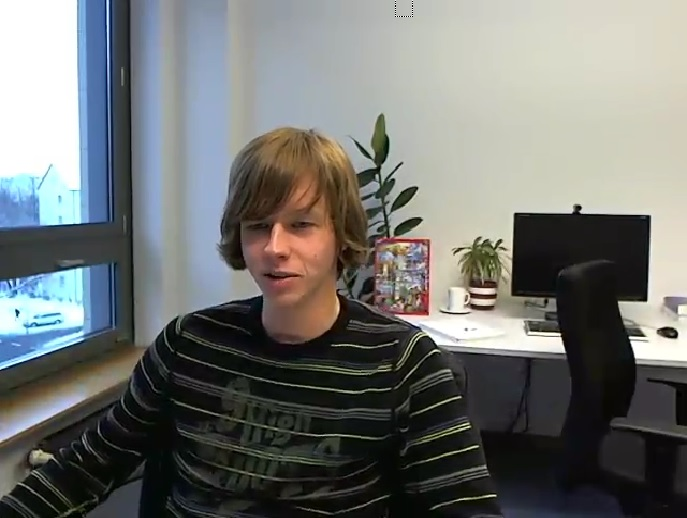
\includegraphics[scale=0.4]{PaulDefault120_91250kbps}
	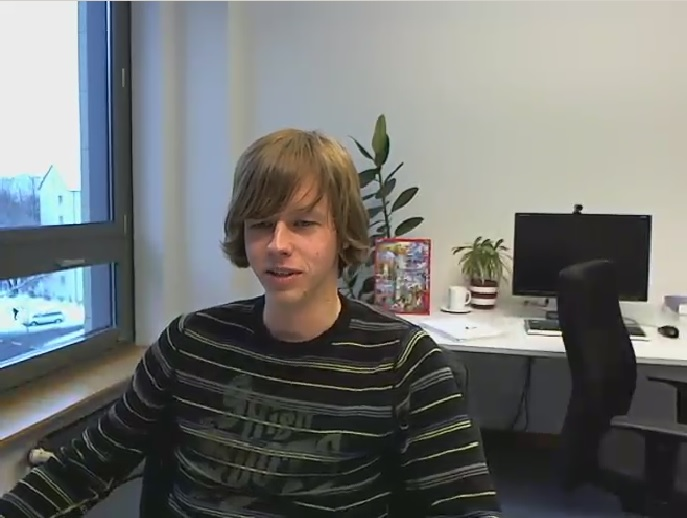
\includegraphics[scale=0.4]{QPOffset/paul120_250kbps_QPoffset4}
	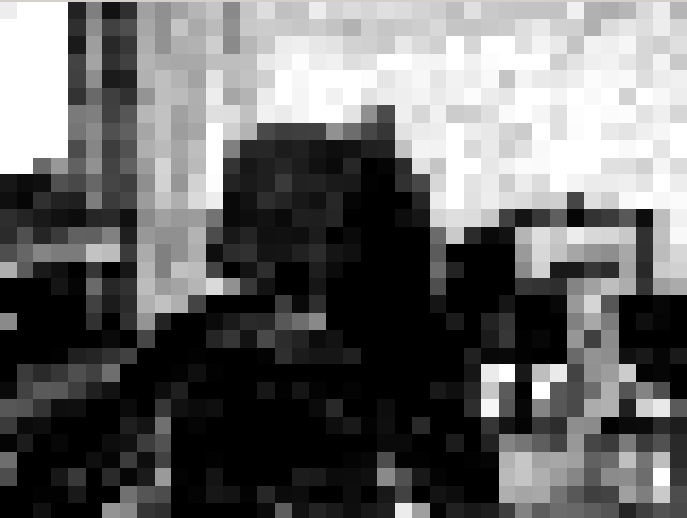
\includegraphics[scale=0.4]{PaulDefault120_91250kbps_psnr}
	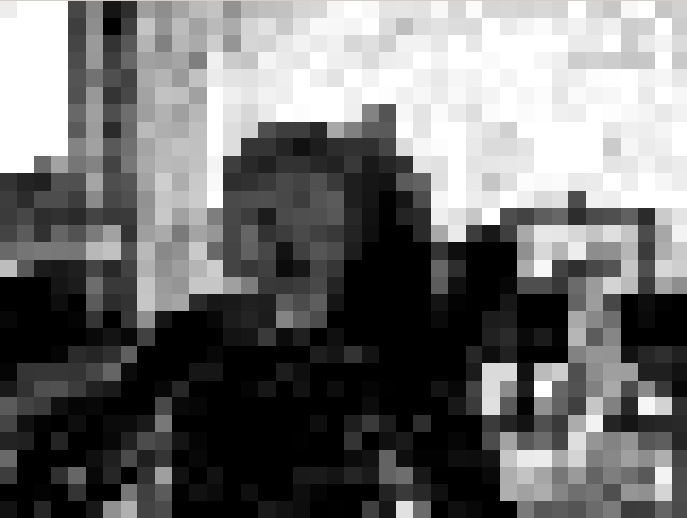
\includegraphics[scale=0.4]{QPOffset/paul120_250kbps_QPoffset4_psnr}
	
\includegraphics[scale=0.37]{PaulDefault120_91250kbps_quant}
	
\includegraphics[scale=0.4]{QPOffset/paul120_250kbps_QPoffset4_quant}    
	\caption{Comparing the images with QP offset of 4 for ROI}
	\label{fig:Default_QPOffsetCompareold}
\end{figure}
\fi

%Replacing Paul with chet640x480
%\begin{figure}
%	\centering
%	\begin{subfigure}[t]{0.45\textwidth}
%		\centering
%		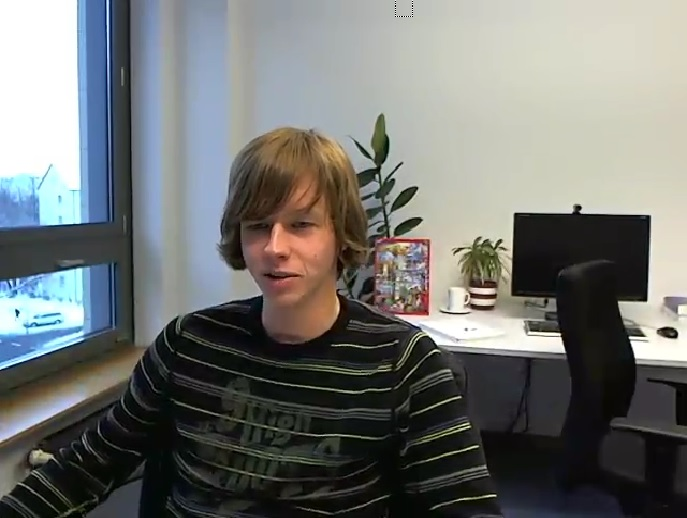
\includegraphics[width=\textwidth]{PaulDefault120_91250kbps}
%		\caption{}
%		\label{fig:QP Offset image comparison 1}
%	\end{subfigure}
%	\begin{subfigure}[t]{0.45\textwidth}
%		\centering
%		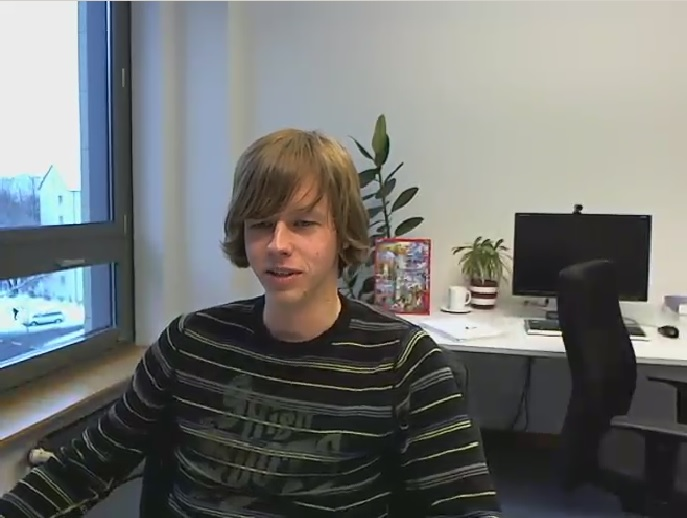
\includegraphics[width=\textwidth]{QPOffset/paul120_250kbps_QPoffset4}
%		\caption{}
%		\label{fig:QP Offset image comparison 2}
%	\end{subfigure}
%	\begin{subfigure}[t]{0.45\textwidth}
%		\centering
%		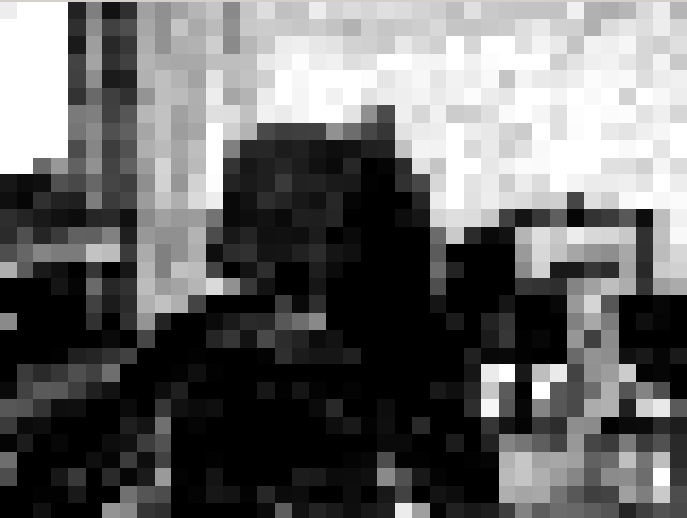
\includegraphics[width=\textwidth]{PaulDefault120_91250kbps_psnr}
%		\caption{}
%		\label{fig:QP Offset PSNR comparison 1}
%	\end{subfigure}
%	\begin{subfigure}[t]{0.45\textwidth}
%		\centering
%		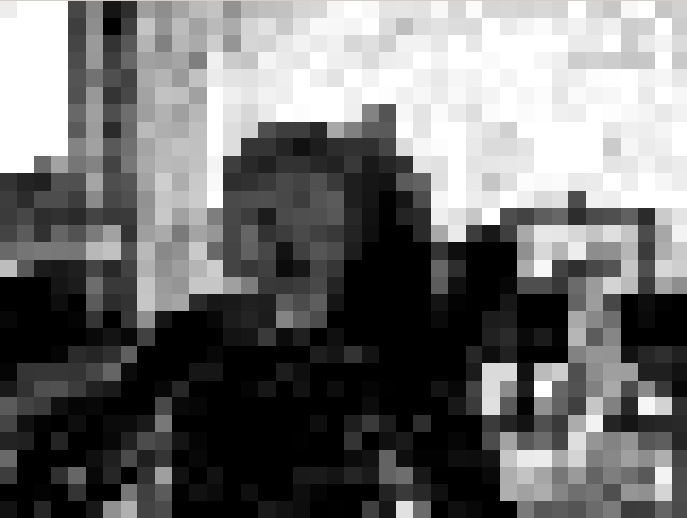
\includegraphics[width=\textwidth]{QPOffset/paul120_250kbps_QPoffset4_psnr}
%		\caption{}
%		\label{fig:QP Offset PSNR comparison 2}
%	\end{subfigure}
%	\begin{subfigure}[t]{0.45\textwidth}
%		\centering
%		
\includegraphics[width=\textwidth]{PaulDefault120_91250kbps_quant}
%		\caption{}
%		\label{fig:QP Offset Quant comparison 1}
%	\end{subfigure}
%	\begin{subfigure}[t]{0.45\textwidth}
%		\centering
%		
\includegraphics[width=\textwidth]{QPOffset/paul120_250kbps_QPoffset4_quant}
%		\caption{}
%		\label {fig:QP Offset Quant comparison 2}
%	\end{subfigure}
%	\caption{The Comparison of conventional encoding and ROI-based encoding with QP offset of 4 for ROI. The figures (a), (c), (e) and  (b), (d), (f) correspond to conventional encoding and QP offset based ROI-encoding approaches respectively. (a), (b) are snapshots from the encoded output. (c), (d) are PSNR maps and (e), (f)  are Quantization maps corresponding frames in (a) and (b).}
%	\label{fig:Default_QPOffsetCompare}
%\end{figure}
%\begin{figure}[!h]
%	\centering
%	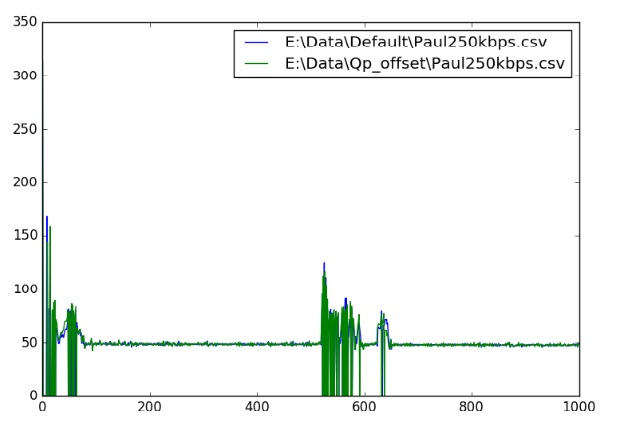
\includegraphics[scale=0.75]{QPOffset/Paul250kbps_QP_Offset_Delay}
%	\caption{Delay plot for conventional encoding and ROI-based encoding with QP offset of 4 for ROI}
%	\label{fig:DelayDefault_QPOffsetCompare}
%\end{figure}
\begin{figure}
	\centering
	\begin{subfigure}[t]{0.45\textwidth}
		\centering
		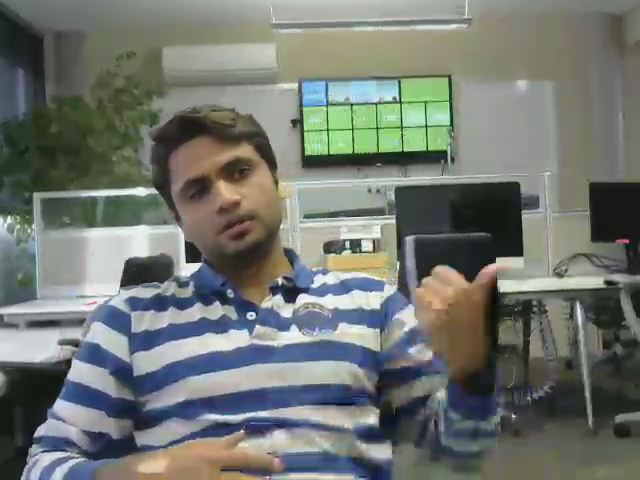
\includegraphics[width=\textwidth]{New_dec/Default/Chet106_250kbpsDefault.png}
		\caption{}
		\label{fig:QP Offset image comparison 1}
	\end{subfigure}
	\begin{subfigure}[t]{0.45\textwidth}
		\centering
		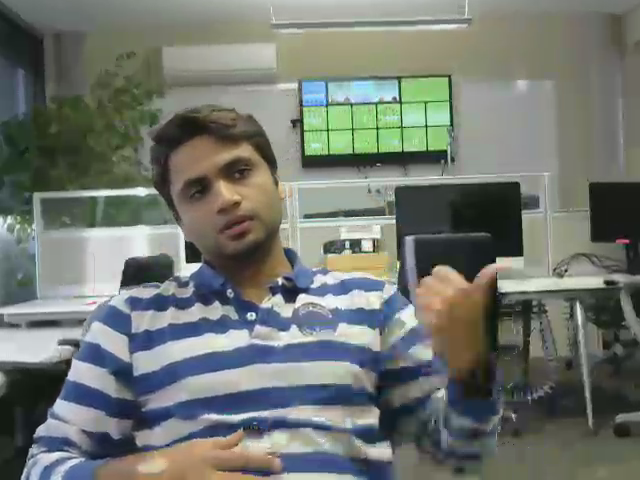
\includegraphics[width=\textwidth]{Tuning_QP_offset/New/-4/Chet250kbpsQpOffsetsingle.png}
		\caption{}
		\label{fig:QP Offset image comparison 2}
	\end{subfigure}
	\begin{subfigure}[t]{0.45\textwidth}
		\centering
		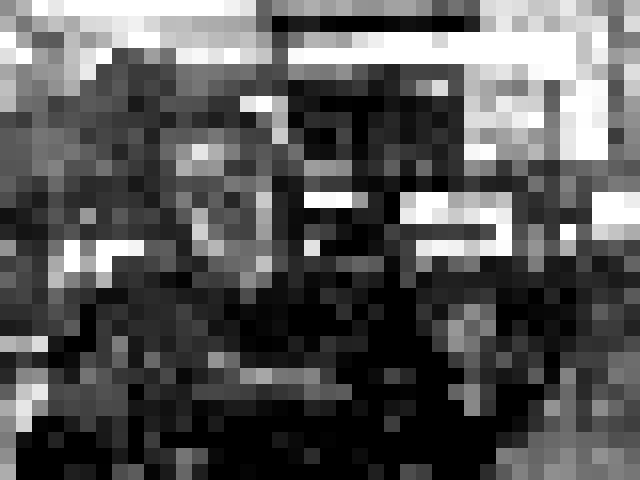
\includegraphics[width=\textwidth]{New_dec/Default/Chet106_250kbpsDefaultPsnrAbs.png}
		\caption{}
		\label{fig:QP Offset PSNR comparison 1}
	\end{subfigure}
	\begin{subfigure}[t]{0.45\textwidth}
		\centering
		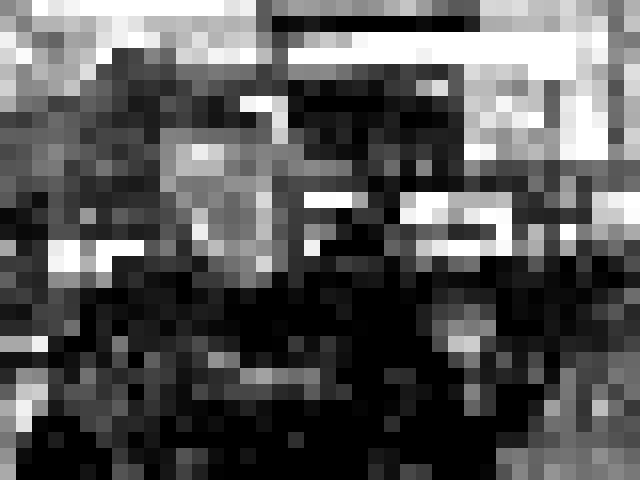
\includegraphics[width=\textwidth]{Tuning_QP_offset/New/-4/Chet250kbpsQpOffsetsinglePsnrAbs.png}
		\caption{}
		\label{fig:QP Offset PSNR comparison 2}
	\end{subfigure}
	\begin{subfigure}[t]{0.45\textwidth}
		\centering
		
\includegraphics[width=\textwidth]{New_dec/Default/Chet106_250kbpsDefaultQuant.png}
		\caption{}
		\label{fig:QP Offset Quant comparison 1}
	\end{subfigure}
	\begin{subfigure}[t]{0.45\textwidth}
		\centering
		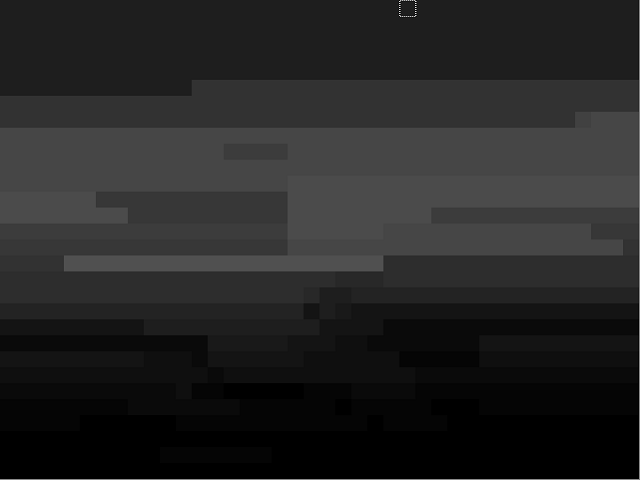
\includegraphics[width=\textwidth]{Tuning_QP_offset/New/-4/Chet250kbpsQpOffsetsingleQuant.png}
		\caption{}
		\label {fig:QP Offset Quant comparison 2}
	\end{subfigure}
	\caption{The Comparison of conventional encoding and ROI-based encoding with QP offset of 4 for ROI. The figures (a), (c), (e) and  (b), (d), (f) correspond to conventional encoding and QP offset based ROI-encoding approaches respectively. (a), (b) are snapshots from the encoded output of Chet640x480. (c), (d) are PSNR maps and (e), (f)  are Quantization maps corresponding to the frames in (a) and (b).}
	\label{fig:Default_QPOffsetCompare}
\end{figure}
\begin{figure}[!h]
	\centering
	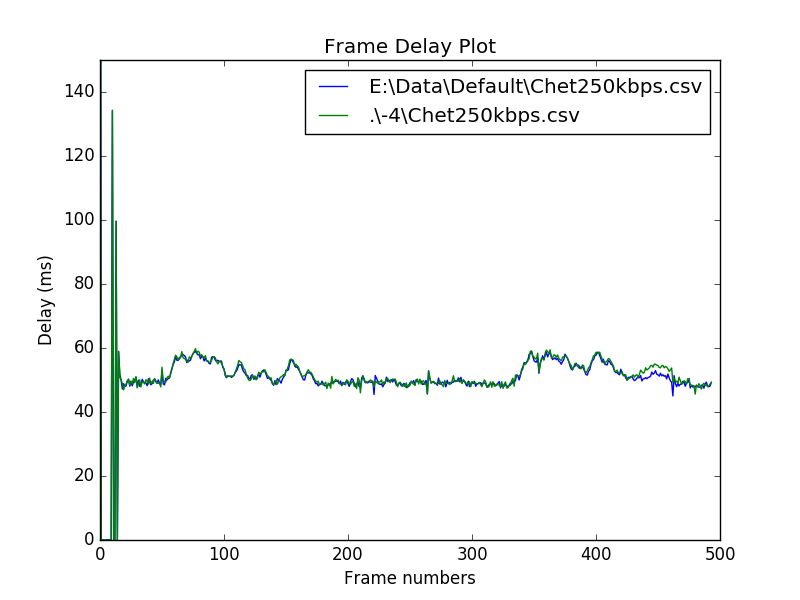
\includegraphics[scale=0.75]{Tuning_QP_offset/New/-4/Chet250kbpsQpOffsetsingleDelay.png}
	\caption{Delay plot for conventional encoding and ROI-based encoding with QP offset of 4 for ROI (Purple - Conventional encoding, Green - QP offset based ROI encoding)}
	\label{fig:DelayDefault_QPOffsetCompare}
\end{figure}

\subsection{Conventional and ROI-based encoding Comparison}
The images in Figure \ref{fig:Default_QPOffsetCompare} shows the comparison between conventional encoding and ROI-based encoding using QP offset and their corresponding attributes like PSNR map and  quantization map. A QP offset ($dq_{roi}$) of 4 was used during ROI-based encoding. The image in Figure \ref{fig:QP Offset image comparison 2} looks better in the face regions compared to Figure \ref{fig:QP Offset image comparison 1} due to usage of negative QP offset for ROI. This improves the overall perceptual quality of the video. Figure \ref{fig:QP Offset Quant comparison 1}-\ref{fig:QP Offset Quant comparison 2} shows the effect of QP offset on the final QP used for encoding the macroblock. The macroblocks in the face region of \ref{fig:QP Offset Quant comparison 2} have lower QP which is seen as  macroblocks with a lighter shade of gray compared to the other macroblocks in the frame. 

The PSNR maps in Figure \ref{fig:QP Offset PSNR comparison 1}-\ref{fig:QP Offset PSNR comparison 2} shows that the PSNR of the face region is improved considerably with ROI-based encoding using QP offset. There is no major difference in PSNR of the background region (non-ROI). The face appears sharper due to the additional boost in quality from reduced QP. The overall bitrate of both the compared bitstreams remained almost equal. The difference in the perceptual quality is only due to the movement of bits from non-ROI to ROI macroblocks. 

Figure \ref{fig:DelayDefault_QPOffsetCompare} shows the delay plot described in section \ref{sec: setup delay plots} for both conventional and ROI-based encoding using QP offset. The visibility of a single color predominantly (due to overlapping) shows that there is no significant change in the bit-consumption at the frame level. This implies that the additional bits consumed by the ROI macroblocks are compensated in non-ROI blocks within a given frame. There is very less difference in bit-consumption at the frame level that is carried over to the next frame. There is no significant change in the number of dropped frames which are represented as zero points in the delay plot. The number of dropped frames with conventional and ROI-based encoding remains the same. The dropped frames also appear at the same time interval in both output bitstreams.

\begin{table} [h!]
	\centering
	\begin{tabular}{ |c|c|c|c|c| }
		\hline
		& & \multicolumn{3}{c|}{PSNR (dB)} \\\cline{3-5}
		QP Offset & Content & Frame & ROI& non-ROI \\
		\hline
		-4 & Chet640x480, 250kbps & 31.22 & 34.27 & 31.04\\   
		-8 & Chet640x480, 250kbps & 30.87 & 35.51 & 30.64\\   
		-12 & Chet640x480, 250kbps & 30.39 & 36.54 & 30.13\\  
		\hline 
	\end{tabular}
	\caption{PSNR Comparison for for QP offset based ROI encoding}
	\label{Table:QPOffsetPsnr}
\end{table}

The PSNR of ROI-based encoding with QP offset is tabulated in Table \ref{Table:QPOffsetPsnr}. There is a considerable improvement in the PSNR of ROI. There is a corresponding drop in PSNR of non-ROI which is reflected in reduced overall frame PSNR. The drop is not significant leading to a overall increased perceptual quality.
%The ROI PSNR is closer to the overall frame PSNR with ROI-based encoding compared to the conventional encoding results shown in Table \ref{InitPSNR1} (section \ref{sec:setup-PSNR}). 

The boost in ROI PSNR is dependent on the magnitude of QP offset used for the ROI macroblocks. A QP offset of -4 might not be optimum QP offset for all the contents. Therefore, It is necessary to consider following aspects during QP offset computation to achieve optimal PSNR for ROI and non-ROI parts resulting in improved perceptual quality. 
\begin{itemize}
	\item Tuning QP offset - Understanding the effect of using different QP offsets.
	\item Area of ROI - The relative area of ROI and non-ROI parts in a frame.
	\item Bi-direction QP offset - A positive QP offset is used for non-ROI blocks along with negative QP offset for ROI.
\end{itemize}

The following section discusses each of these aspects in detail to form a generic QP offset computation approach applicable to most of the contents.


%which However, this approach might result in bitrate control over-reacting for the blocks around the ROI and encode them with extremely low quality. The magnitude of QP offset shall dictate the magnitude of shift in quality for the ROI. This approach is used to find right QP offset for best perceptual quality.\\
%
%It is perhaps a better idea to link the confidence quotient of face detection algorithms with the QP offset used. It should also be dependent on the area of the face, if the area of the ROI is considerably large in a video then the quality difference should be minimized. This is because there will be less non-ROI regions to compensate for additional bits used in ROI.



%
\subsection{Tuning QP Offset} \label{sec:Tuning QP Offset}
As mentioned earlier, the ROI-based encoding approaches discussed in this work only aim to re-distribute the bits within a frame based on the region of interest. The magnitude of re-distribution should be carefully chosen to avoid degradation of the background to an extent that artifacts become noticeable to the viewer even though those regions are not of primary importance to the viewer. An ideal redistribution of bits will make sure that there is a maximum transfer of bits from non-ROI part to ROI part without creating any visible artifacts in the non-ROI parts of the image.

%\begin{figure}[!h]
%	\centering
%	\includegraphics[scale=0.43]{QPOffset/trialOffset/Paul250kbps_offset2}
%	\includegraphics[scale=0.43]{QPOffset/trialOffset/Paul250kbps_offset4}
%	\includegraphics[scale=0.43]{QPOffset/trialOffset/Paul250kbps_offset6}
%	\includegraphics[scale=0.43]{QPOffset/trialOffset/Paul250kbps_offset8}  
%	\caption{Tuning QP offset - Trial QP offsets used are 2, 4, 6 and 8 in raster scan order}
%	\label{fig:Default_QPOffsetTuning}
%\end{figure}



%
\begin{figure}[h!]
	\centering
	\begin{subfigure}[t]{\textwidth}
		\centering
		\includegraphics[width=0.49\textwidth]{Tuning_QP_offset/New/-8/Chet250kbpsQpOffsetsingle.png}
		\includegraphics[width=0.49\textwidth]{Tuning_QP_offset/New/-8/Chet250kbpsQpOffsetsinglePsnrAbs.png}
		\caption{QP offset = -8}
		\label{fig:QP offset compare 8}
	\end{subfigure}
	\begin{subfigure}[t]{\textwidth}
		\centering
		\includegraphics[width=0.49\textwidth]{Tuning_QP_offset/New/-12/Chet250kbpsQpOffsetsingle.png}
		\includegraphics[width=0.49\textwidth]{Tuning_QP_offset/New/-12/Chet250kbpsQpOffsetsinglePsnrAbs.png}
		\caption{QP offset = -12}
		\label{fig:QP offset compare 12}
	\end{subfigure}
	\caption{The snapshot of ROI-encoded Chet640x480 (Left) and its corresponding absolute PSNR map (Right) for different QP offsets.}
	\label{fig:QP offset tuning}
\end{figure}
In this work, various offsets were used to study the effect of magnitude of QP offset on perceptual quality. The results of ROI-based encoding with QP offset of -4 shows favorable results with increased perceptual quality. This section examines the impact of increasing the magnitude of QP offset further. %The results shown in Figure \ref{fig:QP offset tuning} shows that, as QP offset increases the face region appears more sharper which improves the overall perceptual quality of the frame. 

The snapshot of same sample input encoded  with QP offset of -8 shown in Figure \ref{fig:QP offset compare 8} has a sharper face region compared to same fame encoded with QP offset of -4 shown in Figure \ref{fig:QP Offset image comparison 2}. This is expected since the face region is coded with a lower QP due to a larger negative QP offset. The blockiness in the non-ROI, specifically around the arm region has increased. The increase in sharpness in face region masks this blockiness to some extent. However, with further increase in the magnitude of QP offset the blockiness in the background becomes more prominent. The image in Figure \ref{fig:QP offset compare 12} is encoded with QP offset of -12. At this point, the increase in sharpness in the face region is masked by extreme blockiness in the non-ROI, specifically around the arm region. It is clear from the images in Figure \ref{fig:QP offset tuning}. The corresponding PSNR plots show extreme low PSNR in the non-ROI with increasing QP offsets. Therefore, a very high QP offset can have adverse effect on the perceptual quality.

%Table to show number of dropped frames
\begin{table} [h!]
	\centering
	\begin{tabular}{ |c|c|c| }
		\hline
		{} & \multicolumn{2}{c|}{\textbf{Encoding Mode}} \\\cline{2-3}	
		\textbf{ROI QP Offset} & \textbf{Swing Restriction = on} & \textbf{Swing Restriction = off} \\
		\hline 
		0 & 16 & 12  \\

		-4 & 19 & 12  \\

		-8 & 31 & 12 \\ 

		-12 & 45 & 14 \\ 
		\hline						
	\end{tabular}
	\caption{Number of dropped frames with different QP offsets for ROI for test sequence with 1000 frames.}
	\label{Table:QP tuning dropped frames}
\end{table}
%\begin{table} [h!]
%	\centering
%	\begin{tabular}{ |c|c|c| }
%		\hline
%		{} & \multicolumn{2}{c|}{\textbf{Encoding Mode}} \\		
%		\textbf{ROI QP Offset} & \textbf{Swing Restriction = on} & \textbf{Swing Restriction = off} \\
%		\hline 
%		0 & 16 & 10  \\
%		\hline
%		-4 & 19 & 11  \\
%		\hline
%		-8 & 31 & 11 \\ 
%		\hline
%		-12 & 45 & 11 \\ 
%		\hline						
%	\end{tabular}
%	\caption{Number of dropped frames with different QP offsets for ROI for test sequence with 1000 frames.}
%	\label{Table:QP tuning dropped frames}
%\end{table}

\subsubsection*{QP Swing Restriction}
It is possible to preserve the quality of the non-ROI macroblocks even with high QP offsets by using QP swing restriction discussed in section \ref{sec: Bitrate overview: Bitrate deviation}. The maximum value of macroblock QP ($QP_{max}$) given by \cref{Eq:QP swing restriction}, avoids the excessive degradation of the non-ROI macroblocks due to the usage of large QP offset. The QP of non-ROI blocks is not allowed to go very high despite over-consumption of bits by ROI blocks.  The side-effects of increased QP offset shows up in the form of an increase in the number of dropped frames. Table \ref{Table:QP tuning dropped frames} shows the number of dropped frames in the encoded video with 400 input frames. There is a drastic increase in the number of dropped frames with QP offset of -8 and -12. This increase in dropped frames reduces the smoothness of the playback which is annoying to the viewer.

When the QP swing restriction was turned off, the number of dropped frames with increased QP offset reduced drastically as shown in Table \ref{Table:QP tuning dropped frames}. There was no considerable increase in the number of dropped frames compared to the output of conventional encoding without using any ROI information. However, the quality of non-ROI blocks dropped significantly without QP swing restrictions as shown in Figure \ref{fig:QP offset tuning}. The extreme blockiness in the non-ROI decreased the perceptual quality. Therefore, using large QP offsets can lead to less perceptual quality either due to increased dropped frames or excessive blockiness in the background depending on the configuration of QP swing restriction. Therefore, the QP offset for the ROI should be tuned not only considering the degradation of the background quality but also by assessing any other side-effects like an increase in the number of dropped frames.

%
%Discuss the impact of ratio of ROI mbs to non-ROI mb's
\subsection{Area of Region of Interest} \label{sec:QP offset area of ROI}
This section discusses the importance of considering the relative area of ROI with respect to the non-ROI parts($A_{roi}$) in computing the QP offsets. The variation in QP offsets discussed in the above section corresponds to a frame with relatively smaller ROI area compared to the whole frame. In this frame, 64 macroblocks out of a total of 1200 macroblocks belong to the face region(ROI). Therefore, the ROI is less than 5 percent of the entire video frame ($A_{roi} < 0.05$). For a small percentage of ROI blocks, it is possible to use a large QP offset (very low ROI QP) since there are large number of non-ROI macroblocks to compensate for the over-consumption of bits by ROI macroblocks. 
 
\begin{figure}[h!]
	\centering
	\begin{subfigure}[t]{0.49\textwidth}
	%	\centering
		\includegraphics[width=0.49\textwidth]{varyingFaceSize/Chet119.png}
	%	\caption{}
	%	\label{}
	%\end{subfigure}
	%\begin{subfigure}[t]{0.24\textwidth}
	%	\centering
		\includegraphics[width=0.49\textwidth]{varyingFaceSize/Chet119_facemap.png}
		\caption{}
		\label{}
	\end{subfigure}
	\begin{subfigure}[t]{0.49\textwidth}
	%	\centering
		\includegraphics[width=.49\textwidth]{varyingFaceSize/Chet446.png}
	%	\caption{}
	%	\label{}
	%\end{subfigure}
	%\begin{subfigure}[t]{0.24\textwidth}
	%	\centering
		\includegraphics[width=0.49\textwidth]{varyingFaceSize/Chet446_facemap.png}
		\caption{}
		\label{}
	\end{subfigure}
	\caption{The snapshots and corresponding face map of frame number 119 with $A_{roi} = 0.675$(a) and frame number 446 with $A_{roi} = 0.35$(c) in sample content chet640x480.}
	\label{fig:variable-face-size}
\end{figure}
	
However, in a video conferencing scenario,  based on the focal length of the camera and distance of the participant from the camera, area of the face in the video frame can change significantly. The number of ROI macroblocks can also change within a given input video sequence. The images in Figure \ref{fig:variable-face-size} shows the variation in size of ROI within a video sequence. This demands continuous adaptation of the QP offset to avoid visual artifacts due to the usage of wrong QP offset. For instance, when the area of ROI greater than area of non-ROI($A_{roi} > 0.5$), usage of higher QP offsets will lead to huge over-consumption of bits by ROI due to increased number of ROI macroblocks causing severe degradation in the quality of non-ROI macroblocks. In order to avoid severe degradation of the background, the magnitude of the QP offset should be inversely proportional to the ratio of the number of ROI blocks to non-ROI blocks.

The algorithm implemented to adapt QP offset uses relative area of ROI. The QP offset is calculated using linear relationship described in (\ref{Eq:QP_offset}). This is a heuristic approximation which was found to yield best perceptual quality across many video contents. The scaled QP offset is then clipped to a value of -6 to avoid large QP offsets which can lead to side-effects discussed in the previous section.
\begin{equation}
\label{Eq:QP_offset}
\begin{aligned}
dq_{roi'} = -round\Big(\frac{M}{M_{roi} * 3}\Big), \\
dq_{roi} = clip(dq_{roi'}, -1 , -6),
\end{aligned}	
\end{equation}
where, $dq_{roi}$ is the offset used for ROI blocks, $M$ is the total number of macroblocks in the frame and $M_{roi}$ is the total number of macroblocks marked as ROI. The negative sign in the equation implies that the calculated offset is negative, which results in QP lower than non-ROI blocks. It is also evident from (\ref{Eq:QP_offset}) that a minimum QP offset ($dq_{roi} = -1$) is used if the ROI covers more than two-third of the whole frame. The magnitude of QP offset increases linearly with subsequent decrease in the ROI area.




\subsection{Bi-direction QP-offset} \label{sec:bi-direction QP offset}
The QP offset computed so far is only applied to the ROI macroblocks. The bitrate control module is responsible for compensating the additional bits used in encoding the ROI blocks by increasing the QP of non-ROI blocks. 

As explained in section \ref{sec: Bitrate overview: Bitrate deviation}, the bitrate control uses feedback from the encoder to constantly react to any deviation in the bitrate at the macroblock level. This feedback loop is not aware of the QP offset which is applied externally to the QP computed by bitrate control ($Q_m$). Due to this, the bitrate control reacts to over-consumption of bits by increasing the QP of non-ROI blocks only after encoding the ROI macroblocks. This effect is clearly seen in the quant map of ROI-based encoding in Figure \ref{fig:QP Offset Quant comparison 2}. 

The macroblocks encoded immediately after ROI have larger QP (depicted as a darker shade of gray). Therefore, this approach does not increase the QP of non-ROI blocks uniformly. The non-ROI blocks encoded before ROI blocks have no increase in QP since reaction by rate control to increased deviation in bitrate is not triggered until the ROI macroblocks are encoded. The non-ROI macroblocks encoded after ROI blocks tend to have lower quality than the non-ROI blocks encoded before the ROI blocks. This non-uniform loss of quality in non-ROI blocks is not desirable for good perceptual quality.

%100486:This para can be removed
The non-uniform increase in non-ROI QP also depends on the position of the ROI within the video frame. For instance, consider a content where the ROI part in the frame falls in the bottom right corner of the frame. Assuming that macroblocks are encoded in the raster-scan order, the over-consumption of bits by the ROI part cannot be compensated within that frame. The error is carried over to the next frame. This alters the frame level bit-consumption behavior and can lead to increased number of dropped frames in extreme cases. 

A bi-directional QP offset is used to avoid the behavior described above. The non-ROI blocks are assigned with a positive QP offset, which can compensate the over-consumption in ROI blocks. The non-ROI blocks are encoded with a higher QP even before ROI blocks are encoded. Since the non-ROI blocks from the start of the frame are encoded with a higher QP, there will be a surplus of bits available which can be used in encoding ROI blocks. In an ideal scenario, the negative and positive QP offsets must negate each other's effect resulting in frame level bits being unchanged had the frame been encoded without any offset.

The study in \cite{HighQualityROICodingForVideoConferencing} suggests that for the frame level bitcount to be constant, the average QP of the frame must remain unchanged before and after adding the offsets. This is an observation made after multiple experiments. The QP offset for non-ROI macroblocks used to compensate for negative QP offset used by ROI is given by,
\begin{equation}
\label{Eq:QP_offset_double}
dq_{nroi} = \frac{M_{roi} * dq_{roi}}{M - M_{roi}}
\end{equation}
where, $dq_{nroi}$ is a positive QP offset used for non-ROI blocks when negative QP offset of $dq_{roi}$ is used for ROI blocks (\ref{Eq:QP_offset}). 

The result of QP offset based ROI encoding is discussed in the following section. It should be noted that the term 'QP offset based ROI encoding' or 'bi-direction QP offset approach' refers to the QP offset scheme with all the improvements discussed in the previous \cref{sec:Tuning QP Offset,sec:QP offset area of ROI,sec:bi-direction QP offset}. 
%%Results of Two-sided QP offset
%\begin{figure}
%	\centering
%	\begin{subfigure}[t]{0.49\textwidth}
%		\centering
%		\includegraphics[width=\textwidth]{QPOffset/Bi_direction/Paul250kbps_uni_QP_offset_Bi_4.png}
%		\caption{}
%		\label{fig:Bi-direction QP offset result image}
%	\end{subfigure}
%	\begin{subfigure}[t]{0.49\textwidth}
%		\centering
%		\includegraphics[width=\textwidth]{QPOffset/Bi_direction/Paul250kbps_uni_QP_offset_Bi_4_psnr_abs.png}
%		\caption{}
%		\label{fig:Bi-direction QP offset result psnr}
%	\end{subfigure}
%	\begin{subfigure}[t]{\textwidth}
%		\centering
%		\includegraphics[width=0.49\textwidth]{QPOffset/Bi_direction/Paul250kbps_uni_QP_offset_Bi_4_quant.png}
%		\caption{}
%		\label{fig:Bi-direction QP offset result quant}
%	\end{subfigure}
%	\caption{The results of ROI-based encoding with Bi-direction QP offset.(a) Snapshot of encoded video, (b) absolute PSNR map (range 25dB - 50dB), (c) quantization map}
%	\label{fig:Bi-direction QP offset result}
%\end{figure}

\subsection{Results}
The result of improved QP offset based ROI encoding is shown in \Cref{fig:ChetImageComp,fig:PaulImageComp,fig:JohnnyImageComp}. The improvements include consideration of relative ROI area to compute the QP offset and Bi-direction QP offset discussed in the previous sections. For the sample input Chet640x480, there is clear improvement in the sharpness of the face region with improved QP offset based ROI encoding (\Cref{fig:ChetImageComp-Qpoffsets}) over conventional encoding (\Cref{fig:ChetImageComp-conventional}). The minor drop in PSNR of the non-ROI is masked by the improvements in the face region which improves the overall perceptual quality. Similar trend is observed for other sample input sequences as well.

\begin{description}
	\item[PSNR Value:] The PSNR values for all the sample video sequences with ROI-based encoding using QP offset is tabulated in \Cref{Table:AllPSNR1}. As expected, there is huge improvement in the PSNR of the ROI and q corresponding drop in non-ROI PSNR. The magnitude of drop in non-ROI PSNR is minor compared to the improvement in ROI PSNR. The reason for this observation is that in all the three chosen sample input sequence, the area of ROI is small compared to area of non-ROI ($A_{ROI} < 0.5$). Due to low $A_{ROI}$ the bits saved from quality degradation of non-ROI is used to encode a smaller number of ROI macroblocks with a higher quality leading to asymmetric change in PSNR values.  
	\item[PSNR and Quantization Maps:] The comparison of PSNR and quantization maps between conventional encoding and improved QP offset based ROI-encoding is shown in \Cref{fig:AllPsnrComparison} and \Cref{fig:AllQuantizationComparison} respectively. 
	In a simpler approach with uni-directional QP offset, one of the disadvantages discussed is non-uniform increase in ROI QP. The quantization map shown in \Cref{fig:AllQuantizationComparison-offset-chet} has more uniform increase in QP of non-ROI compared to the approach without bi-direction QP offset shown in \Cref{fig:QP Offset Quant comparison 2}. The regions below ROI do not reach extreme high QP since a positive QP offset is added to non-ROI QP from the start of the frame. This also improves the overall perceptual quality.
	\item[Delay Plots:] The delay plots for improved QP offset approach is shown in \Cref{fig:AllDelayComparison}. For each of the sample video sequence, the delay curve follows very closely the curve for conventional encoding. This shows that the QP offset based approach does not modify the bit-consumption behavior at frame level. The absence of any additional zero-points indicate that there is no increase in the number of dropped frames. This is a highly desirable behavior since it indicates that there will be no glitch in playback of the video due to ROI-based encoding. 	
\end{description}

This section analyses the advantages and disadvantages of ROI-based encoding using QP offsets. Since the QP offset is applied outside the bitrate control, there is less possibility of other factors like buffer fullness and global deviation ($D_m^{n'}$) overriding the QP offset. Such guaranteed QP offsets will ensure boost in the ROI quality at all circumstances. However, this approach has many side effects due to the forced QP offset. The main disadvantage of this approach is not considering the characteristics of the input video content to decide the QP offset. Any given input with a given ratio of the number of ROI blocks to non-ROI blocks will have the same QP offsets irrespective of the content. The QP offset computation is empirical which will work for most of the contents. However, it is not guaranteed to give optimal results for all contents.

The advantages and disadvantages of this approach can be summarized as follows,
\subsection*{Advantages}
\begin{itemize}
	\item Easy to implement with minimal changes required to the encoder.
	\item As shown in the delay plots of \Cref{fig:AllDelayComparison}, there is hardly any change in the frame level behavior of the bitrate control module due to ROI-based encoding.
	\item QP offset is forced irrespective of the buffer conditions, therefore guarantees quality difference between ROI and non-ROI.
\end{itemize}

\subsection*{Disadvantages}
\begin{itemize}
	\item The QP offsets chosen does not take into account any of the input content characteristics. Same QP offset is used for all the contents for a given ROI to non-ROI ratio.	
	\item Since buffer conditions are not considered at macroblock level, there is an increased possibility of dropped frames.
	%%	\item The reaction of the bitrate control to external offset is not uniform throughout the non-ROI macroblocks. The reaction is less before encoding the ROI and very high just after encoding the non-ROI. This causes non uniform quality within the non-ROI macroblocks. 
	\item The deviation control mechanism described in section \ref{sec: Bitrate overview: Bitrate deviation} is not in sync with QP offsets. The deviation control mechanism will increase the QP even for ROI blocks when there is an increased deviation due to over-consumption of bits by ROI macroblocks.
\end{itemize}

The next section introduces an alternative approach for ROI-based encoding using ROI-based bit-allocation scheme. Some of the disadvantages of the QP offset approach are addressed in the new approach.

%%Add new section for splitting bit-allocation
%%Second and most complex appraoch
\section{ROI based Bit-Allocation}
This section introduces an approach with modifications to the bit-allocation module for improved ROI-based encoding. The main drawback of the QP offset based approach is that the input video content characteristics are not considered for determining the QP offset. The difference in complexity of ROI and non-ROI macroblocks determines the magnitude of quality difference required for good perceptual quality. This magnitude of optimal quality difference varies across different contents depending on the variation in complexity within a frame. For instance, consider a sample input video with complex background with some temporal complexity(non-ROI) but a simple static foreground (ROI). The usage of heuristic QP offsets which assumes background to be mostly static will result in annoying blocky artifacts in the background. This might decrease the perceptual quality to a level below that of conventional encoding. Therefore, it is important to consider the relative complexities of ROI and non-ROI parts to compute the desired quality difference between these regions.

In conventional encoding, the bit-consumption is not uniform across all the macroblocks even though all regions of a frame are considered equally important to the viewer. This is due to variation in complexities across different macroblocks. The image in Figure \ref{fig:DefaultJohnnyBitConsumption} shows relative macroblock size in bits for a conventionally encoded frame. Similar to quant and PSNR maps, the brighter shade of gray represents larger bit-consumption. It is clear that background regions consume least amount of bits and face region consumes an above average amount of bits. A bit-allocation strategy for ROI-based encoding which allocates higher than average amount of bits to ROI based on arbitrary weights \cite{ROI-MV-based-face-tracking,ROI-resource-allocation} might not allocate any additional bits compared to the conventional encoding. For ROI-based encoding, the bit-allocation strategy should take into account the relative complexities of ROI and non-ROI and allocate bits with a bias over the complexity based bit-allocation. The fundamental idea behind this approach is to allocate bits to ROI and non-ROI proportional to their complexities with an additional bias for ROI.
\begin{figure}[h!]
	\centering
	\includegraphics[scale=0.4]{New_dec/Johnny_Default_bit_consumption.png}
	\caption{Macroblock level bit-consumption for Johnny1280x720 (Conventional encoding).}
	\label{fig:DefaultJohnnyBitConsumption}
\end{figure}

In this approach, the bits allocated at frame level $(B_{alloc})$ is split between ROI and non-ROI parts based on the relative complexities of these regions. The cost of a macroblock computed during rate-distortion optimization (\ref{Eq:CostCalc}) is accumulated for ROI and non-ROI regions to get the relative complexity ($C_r$),
$$C_r = \frac{\sum_{i =0}^{M_{roi}}{J_i}}{\sum_{i =0}^{M-M_{roi}}{J_i}},$$
where, $J_i$ is the RDO cost of the macroblock $i$. The cost of a region determines the bits consumed by the corresponding region. The relative bit consumption of ROI and non-ROI is predicted assuming that,
\begin{equation}
\label{Eq:Relative bit consumption}
C_r \propto B_R,
\end{equation}
where, $$B_R = \frac{B_{roi}}{B_{nroi}}.$$
Here $B_{roi}$ and $B_{nroi}$ are the accumulated bit consumption of $M_{roi}$ macroblocks belonging to ROI and  $M_{nroi}$ non-ROI macroblocks respectively. The above equations hold true for any two regions in a given frame given that these two regions are encoded with equal importance (no ROI-encoding). Therefore, $B_{roi}$ and $B_{nroi}$ corresponds to bit consumption of the two regions if the frame was encoded conventionally without using any ROI information. The idea is to predict the bit-consumption in conventional encoding and allocate bits for ROI and non-ROI regions according to the estimate but with an additional bias for the ROI part. 

The ROI-based bit-allocation involves following major steps.
\begin{itemize}
	\item \textit{Relative Bit-consumption Prediction} - Predict relative bit-consumption of ROI and non-ROI ($B_R$) in conventional encoding.
	\item \textit{ROI and non-ROI Bit Allocation} -  Split allocated frame level bits ($B_{alloc}$) between ROI and non-ROI parts according to $B_R$ with an additional bias for ROI parts.
	\item \textit{Region-based bitrate control} - Independent bitrate control for ROI and non-ROI regions.
\end{itemize}
The following sections discuss each of the above steps in detail.

\subsection{Relative Bit-consumption Prediction} \label{sec:Relative Bit-consumption Prediction}
The first step in ROI based bit-allocation is to determine the relative bit-consumption of the ROI and non-ROI parts ($B_R$) if the frame was encoded normally without any bias for ROI regions (conventional encoding). There are two possible ways of achieving this,
\begin{enumerate}
	\item Encode a frame using conventional encoding without any bias for ROI, measure the bit-consumption for ROI and non-ROI. The frame can be re-encoded with a bias in bit-allocation for ROI.
	\item Estimate the complexities of ROI and non-ROI parts and use a cost-bits model to predict relative bit-consumption.
\end{enumerate}
The first approach is very inefficient and not suitable for real-time encoding scenario. Therefore, a cost-bits model is used to predict $B_R$.

In this work, the relationship between the complexity of a macroblock and its bit-consumption during conventional encoding is studied. The RDO cost (\ref{Eq:CostCalc}) is chosen as the complexity metric for prediction of $B_R$. The computation of a new complexity metric for predicting bit-consumption is not desirable due to increased complexity. The RDO cost which is computed by the encoder during rate-distortion optimization stage is reused to predict $B_R$. 

\subsubsection*{Effect of RDO Cost on bit-consumption}
The cost of a macroblock affects its bit-consumption in two opposite ways listed below. 
\begin{itemize}
	\item The cost of a macroblock reflects the complexity of the macroblock. A macroblock with a higher cost consumes more bits (\ref{Eq:Relative bit consumption}).
	\item The RDO cost is also used in the bitrate control for delta QP prediction as discussed in section \ref{used QP prediction overview}. The delta QP computation (\ref{Eq:deltaQP}) allocates a higher QP to the macroblock with a higher cost for spatial and temporal masking considering HVS. This will marginally reduce the bit-consumption of the macroblock.
\end{itemize}
These conflicting influence of cost on bit-consumption makes its prediction more complex. In this work, the effect of delta QP on bit-consumption is ignored for simplicity. A cost-bits model is developed assuming no variation in QP across the macroblocks.

\subsubsection{Cost-Bits Model}
A model to relate cost of a macroblock and its bit-consumption is developed using data from multiple video conferencing sequences. Figure \ref{fig:CostvsBits_ConstQP_Full} shows the plot of cost vs bits at the macroblock level. Every point on this plot corresponds to bit-consumption of a macroblock and its corresponding RDO cost computed during the RDO stage. The plot corresponds to all the macroblocks in the encoded video sequences with 50 frames each from four different video conferencing samples. The sample input sequences used for evaluation (listed in section \ref{sec:sampleInput}) are not included for developing the model for a fair evaluation. The input video sequence used for developing the model and the ones used for evaluating the model are different. The encoding for this plot was done in constant QP mode with QP=35 for all the macroblocks. The data of the first key frame is not included in this plot since the first key frame is encoded without using any ROI information. It can be noticed that there is a linear relationship between predicted macroblock cost and the corresponding bit-consumption.


%In the first iteration, constant QP across all the macroblocks in a frame is used for coarse prediction of relative bit-consumption from the RDO-cost.

\begin{figure}[h!]
	\centering
	\includegraphics[scale=0.75]{CostVsBits/new/CostvsBits_ConstQP_global_all.png}  
	\caption{Macroblocks cost vs bits plot for all the macroblocks of multiple video sequences}
	\label{fig:CostvsBits_ConstQP_Full}
\end{figure} 

The linear relationship between cost of a macroblock (J) and its corresponding bit-consumption (b) at a constant QP is given by,
\begin{equation}
\label{Eq:costvsbits model all}
J = 18.2 . b + 693.
\end{equation}
The above equation is obtained by performing linear regression on the entire data set shown in Figure \ref{fig:CostvsBits_ConstQP_Full}. It has a corresponding $R^2$ value of 0.2366. The $R^2$ value (also displayed on the plots) is a measure of correlation between actual data and the predicted data using the linear relationship. A value of $R^2 = 1$ indicates perfect correlation. The $R^2$ value in this case is lower to form an efficient prediction model. The correlation between macroblock cost and its bit-consumption is increased further by considering the prediction mode of the macroblock.

\subsubsection*{Cost-Bits Model - Prediction Modes}

The data in Figure \ref{fig:CostvsBits_ConstQP_Full} includes data for macroblocks of all types of prediction modes like skip, intra and inter prediction. It was observed that the predictability of bit-consumption using RDO cost was heavily dependent on the prediction mode used for encoding the macroblock. 

The analysis of the macroblock cost and its corresponding bit-consumption specific to a prediction mode is shown in Figure \ref{fig: Cost vs bits mode}. The plots in Figure \ref{fig: Cost vs bits mode} are generated using the same data as shown in Figure \ref{fig:CostvsBits_ConstQP_Full}. Different plots are generated for skip, inter and intra prediction modes. It can be noticed that the correlation between the macroblock cost and its bit-consumption is maximum for intra-prediction ($R^2 = 0.8757$) followed by inter-prediction ($R^2 = 0.2995$). However, the bit-consumption pattern was found to be almost independent of the cost for skip-mode macroblocks ($R^2 = 0.0412$). This is because skip-mode decision happens in a later stage of encoding when there are no transform coefficients generated for a macroblock encoded with intra or inter-prediction. The cost associated with skip macroblock corresponds to the prediction mode chosen before the macroblock was decided to be encoded as skip macroblock.

%Table to encoding mode specific data
\begin{table} [h!]
	\centering
	\begin{tabular}{ |c|c|c| }
		\hline
		\textbf{Prediction Mode} & \textbf{Occurrence Probability } & \textbf{$R^2$ value} \\
		\hline 
		Intra & 0.233 & 0.8757  \\
		\hline
		Inter & 0.28 & 0.2995  \\
		\hline
		Skip &  0.69 & 0.0412 \\ 
		\hline					
	\end{tabular}
	\caption{The probability of prediction modes in constant QP (QP = 35) and its corresponding $R^2$ value.}
	\label{Table:Mode Specific data}
\end{table}

%Complexity vs bits prediction analysis
%%Results of Two-sided QP offset
\begin{figure} [h!]
	\centering
	\begin{subfigure}[t]{0.49\textwidth}
		\centering
		\includegraphics[width=\textwidth]{CostVsBits/const_QP/CostvsBits_ConstQP_inter.png}
		\caption{Inter Prediction mode}
		\label{fig: Cost vs bits mode inter}
	\end{subfigure}
	\begin{subfigure}[t]{0.49\textwidth}
		\centering
		\includegraphics[width=\textwidth]{CostVsBits/const_QP/CostvsBits_ConstQP_intra.png}
		\caption{Intra Prediction mode}
		\label{fig: Cost vs bits mode intra}
	\end{subfigure}
	\begin{subfigure}[t]{\textwidth}
		\centering
		\includegraphics[width=0.49\textwidth]{CostVsBits/const_QP/CostvsBits_ConstQP_skip.png}
		\caption{Skip mode}
		\label{fig: Cost vs bits mode skip}
	\end{subfigure}
	\caption{The Cost vs Bits plots of macroblocks specific to mode of encoding. (a) inter prediction mode, (b) intra prediction mode, (c) skip mode}
	\label{fig: Cost vs bits mode}
\end{figure}

The data in Table \ref{Table:Mode Specific data} shows the probability of choosing a given prediction mode.  It is clear that skip mode in the most commonly used prediction mode for the encoder configuration discussed in section \ref{sec:Encoder configuration}. This is due to the low target bitrate and mostly static background in video conferencing samples. Therefore, it is very important to have good bits vs cost prediction model for skip macroblocks to compute $B_R$ with a reasonable accuracy.

Fortunately, the extremely low correlation between macroblock cost and its bit-consumption for skip mode can be easily handled by assuming a constant number of bits for skip mode and ignoring its cost. The average amount of bits consumed by the skip macroblocks over the entire data-set was found to be 0.458 bits. This is extremely low bit-consumption compared to the intra and inter mode macroblocks. Therefore, a constant bit-estimate (average bits) is used in (\ref{Eq:Relative bit consumption}) to compute relative bit-consumption of ROI and non-ROI based on the number of skip macroblocks in each of these regions. The $R^2$ value of the prediction model is improved considerably by this assumption for the skip macroblocks.

The steps involved in computing relative bit-consumption of ROI and non-ROI region ($B_R$) are summarized below.
\begin{itemize}
	\item Identify the ROI and non-ROI macroblocks in the input frame.
	\item Get the number of intra, inter and skip macroblocks in the ROI and non-ROI parts separately. This can be done using data from the previous frame.
	\item Compute relative complexity of the ROI and non-ROI parts by accumulating costs of macroblocks in these regions.
	\item The relative complexity ($C_R$) is translated to relative bit-consumption ($B_R$) between ROI and non-ROI using  prediction models shown in Figure \ref{fig: Cost vs bits mode}. A previously trained cost-bits model is used for intra and inter blocks. A pre-computed value is used for the skip macroblocks to account for bits consumed by the skip macroblocks.
\end{itemize}

The procedure involved in using ($B_R$) to allocate bits to ROI and non-ROI parts with a bias for ROI parts to perform ROI-based encoding is discussed in the subsequent sections.

\subsection{ROI and non-ROI Bit Allocation}
This section gives an overview of the process involved in splitting the allocated frame level bits ($B_{alloc}$) computed in (\ref{Eq:bit-allocation}) between ROI($B_{alloc}^{roi}$) and non-ROI($B_{alloc}^{nroi}$) parts. This is done using relative bit-consumption factor ($B_R$) computed in the previous section. The idea behind ROI-based bit allocation is to estimate relative bit-consumption between ROI and non-ROI in conventional encoding, perform bit-allocation according to the estimate with a bias for ROI. The predicted relative bit-consumption between ROI and non-ROI in conventional encoding is given by $B_R$ computed in the previous sections. For ROI-based encoding, a bias factor k is introduced to create bias in bit-allocation. The bias factor signifies the importance of ROI over non-ROI. The bits allocated for ROI region is given by
\begin{equation}
\label{Eq:ROI allocated bits}
B_{alloc}^{roi} = k \times B_R \times B_{alloc}^{nroi}
\end{equation}
and
$$ B_{alloc}^{nroi} = B_{alloc} - B_{alloc}^{roi}$$
Here k is the ROI bias factor. In conventional encoding where all the parts of the frame are considered equally important, $k = 1$. For ROI-based encoding, a value $k > 1$ is used to bias bit-allocation to allocate more bits to ROI considering its importance to the perceptual quality. The bias factor($k$) gives the flexibility of tuning the bias for ROI based on the importance of ROI.

As mentioned earlier, the ROI-based bit-allocation is independent of the procedure involved in determining the relative bit-consumption factor ($B_R$). The approach presented in section \ref{sec:Relative Bit-consumption Prediction} needs computation of relative complexities of ROI and non-ROI regions. A simpler approach is to assume that the frame is uniformly complex and splitting the allocated frame level bits ($B_{alloc}$) uniformly between ROI and non-ROI with bias factor specified in (\ref{Eq:ROI allocated bits}). Therefore, if the content information is not factored in for simplicity, the bits allocated for ROI and non-ROI is computed using (\ref{Eq:ROI allocated bits}) with,
$$B_R = \frac{M_{roi}}{M - M_{roi}}.$$ 
The bias factor k determines the additional bits allocated to the ROI macroblocks. The main advantage of encoding with ROI-based bit-allocation compared to ROI-encoding based on QP offset is that it gives more control to guarantee minimum quality for the background macroblocks (non-ROI). For instance, the value of ROI-bias factor (k) can be bounded in such a way that non-ROI macroblocks are allocated at least half the amount of bits allocated during conventional encoding. This ensures that the quality of non-ROI does not deteriorate to an extent that blockiness in the background reduces the perceptual quality.

In this work, the value of k is chosen to first allocate non-ROI half of the bits it would have consumed in conventional encoding. The excess is allocated to ROI parts. The maximum excess bits allocated to ROI is three times its bit-consumption in conventional encoding. The excess is allocated back to the non-ROI parts. Therefore, the value of k changes depending on the complexities of ROI and non-ROI. 
%if asked for equations for above computations

\subsection{Region based Bitrate Control}
In the previous stages, the procedure for splitting the allocated frame level bits ({$B_{alloc}$}) between ROI and non-ROI is described. The input to this stage is bits allocated for ROI ($B_{alloc}^{roi}$) and non-ROI ($B_{alloc}^{nroi}$) parts. The target is to achieve bit-consumption according to the split between ROI and non-ROI parts with minimal error. 

The bitrate control module described in \cref{chapter:used-bitrate-control-overview} performs only frame level bit-allocation. There is no macroblock level bit-allocation. The task of the bitrate control module was to reduce the error between allocated frame bits $B_{alloc}$ and the frame level bit-consumption without worrying about bit-distribution within a frame. 

In the ROI-based bit-allocation, the bit-allocation is not limited to frame level. The input frame is divided into two regions based on the ROI information and target bits are specified for each of these regions separately. The task of the bitrate control module is to meet bitrate for different regions independently (ROI and non-ROI) with minimal error. This section describes the modifications to the bitrate control module to accomplish this task.

The bitrate control module studied in \cref{chapter:used-bitrate-control-overview} computes the deviation factor ($D_m^{n'}$) based on accumulated error in frame level bit-consumption after encoding every frame as shown in (\ref{Eq:Frame level bit error accumulation}). In steady-state, the deviation factor ($D_m^{n'}$) takes a value such that the error in frame level bit-consumption is minimum. 

The following steps summarize the approach to implement region-based bitrate control using the existing bitrate control described in \cref{chapter:used-bitrate-control-overview}.
\begin{itemize}
	\item Compute the deviation factor for ROI ($Droi_m^{n'}$) and non-ROI ($Dnroi_m^{n'}$) independently. The deviation factors are updated using feedback data from ROI and non-ROI parts independently. This can be visualized as having two instances of rate control running for ROI and non-ROI treating ROI and non-ROI as separate frames.
	\item A single instance of macroblock level bitrate error is maintained as shown in (\ref{Eq:Frame level bit error accumulation}). This ties the two instances of bitrate control together, so that frame level bit-error is minimized. The error in allocation and consumption of bits in the ROI and non-ROI is compensated throughout the frame resulting in less overall frame level error.
	\item The VBV compliance works with frame level bit-allocation and therefore remains unchanged. There will be no increase in number of dropped frames as long as frame level deviation in bit-consumption is kept under check.
\end{itemize} 

%The major problem with two instances of global deviation for ROI and non-ROI, which are simultaneously updated at the end of encoding of a frame is that it can lead to severe oscillations in the frame QP. The error in allocated bits and consumed bits for a given region have opposite effects on two instance of global deviation which results in oscillations of average frame level QP. Figure \ref{fig: ROI bit-alloc oscc} shows the variation in encoded frame size with the usage of two different instances of deviation factor corresponding to ROI and non-ROI parts. The alternative frames differ in size almost by a factor of 2. Such oscillations were observed in steady-state (frame number 400-450 in the example shown). This variation in quality across alternate frames affects the perceptual quality adversely 
%
%The oscillation of the frame average QP was avoided by keeping the update of two instances of deviation factors separate. The deviation factor for ROI and non-ROI is updated at the end of alternate frames. Since, the two updates are not happening simultaneously, there is increased stability resulting in near constant frame level bit consumption as shown in \ref{fig: ROI bit-alloc oscc corrected}.
%
%%Images to show oscillations
%\begin{figure}
%	\centering
%	\begin{subfigure}[t]{\textwidth}
%		\centering
%		\includegraphics[width=\textwidth]{RC_bit_allocation/Oscillation/Paul250kbps_RC_bit_alloc_osc.png}
%		\caption{}
%		\label{fig: ROI bit-alloc oscc}
%	\end{subfigure}
%	\begin{subfigure}[t]{\textwidth}
%		\centering
%		\includegraphics[width=\textwidth]{RC_bit_allocation/Oscillation/Paul250kbps_RC_bit_alloc_corrected_osc.png}
%		\caption{}
%		\label{fig: ROI bit-alloc oscc corrected}
%	\end{subfigure}
%	\caption{A plot of frame size in bits for 50 frames from frame number 400 to 450 for the encoded Paul250kbps content with Bit-allocation based ROI encoding. The two figures vary in approach used to update the deviation factors for ROI and non-ROI regions (a) Simultaneous update (b) Alternate Frame Update}
%	\label{fig: ROI bit-alloc oscc example}
%\end{figure}

%%Results of ROI-based bit-allocation
%\begin{figure}
%	\centering
%	\begin{subfigure}[t]{0.49\textwidth}
%		\centering
%		\includegraphics[width=\textwidth]{RC_bit_allocation/Paul250kbps_ROI_bit_alloc.png}
%		\caption{}
%		\label{fig:ROI bit-allocation result image}
%	\end{subfigure}
%	\begin{subfigure}[t]{0.49\textwidth}
%		\centering
%		\includegraphics[width=\textwidth]{RC_bit_allocation/Paul250kbps_ROI_bit_alloc_psnr_abs45.png}
%		\caption{}
%		\label{fig:ROI bit-allocation result psnr}
%	\end{subfigure}
%	\begin{subfigure}[t]{\textwidth}
%		\centering
%		\includegraphics[width=0.49\textwidth]{RC_bit_allocation/Paul250kbps_ROI_bit_alloc_quant.png}
%		\caption{}
%		\label{fig:ROI bit-allocation result quant}
%	\end{subfigure}
%	\caption{The results of ROI-based encoding using ROI based bit-allocation.(a) Snapshot of encoded video, (b) absolute PSNR map (range 25dB - 50dB), (c) quantization map}
%	\label{fig:ROI bit-allocation result}
%\end{figure}
\begin{table} [h!]
	\centering
	\begin{tabular}{ |c|c|c|c|c| }
		\hline
		& & \multicolumn{3}{c|}{PSNR (dB)}\\ \cline{3-5}
		Methodology & Content & Frame & ROI (dB) &non-ROI\\
		\hline 
		\multirow{3}{*}{\parbox{0.3\linewidth}{Conventional Encoding}} & Paul640x480, 250kbps & 39.15 & 37.72 & 39.22\\ 
							  & Johnny1280x720 350kbps & 37.93 & 36.08 & 38.13\\ 
							  & Chet640x480 250kbps & 31.35 & 32.91 & 31.24\\ 
		\hline
		\multirow{3}{*}{\parbox{0.3\linewidth}{Improved QP Offset based ROI encoding}}  & Paul640x480, 250kbps & 38.29 & 40.10 & 38.24\\ 
											   & Johnny1280x720 350kbps & 37.50 & 37.37 & 37.52\\ 
											   &  Chet640x480 250kbps & 31.08 & 34.89 & 30.89\\ 
		\hline
		\multirow{3}{*}{\parbox{0.3\linewidth}{ROI-based Bit-allocation}} & Paul640x480, 250kbps & 38.22 & 40.95 & 38.15\\ 
								 & Johnny1280x720 350kbps & 36.94 & 38.57& 36.85\\  
								 &  Chet640x480 250kbps & 30.55 & 36.17& 30.30\\
		\hline 
	\end{tabular}
	\caption{PSNR Comparison for different approaches of ROI encoding}
	\label{Table:AllPSNR1}
\end{table}
%% NewImages for comparison
%All methods side-by-sde
\begin{figure}[h!]
	\centering
	\begin{subfigure}[t]{0.49\textwidth}
		\centering
		\includegraphics[width=\textwidth]{New_dec/Default/Chet106_250kbpsDefault.png}
		\caption{}
		\label{fig:ChetImageComp-conventional}
	\end{subfigure}
	\begin{subfigure}[t]{0.49\textwidth}
		\centering
		\includegraphics[width=\textwidth]{New_dec/Qp_offset/Chet106_250kbpsQpOffset.png}
		\caption{}
		\label{fig:ChetImageComp-Qpoffsets}
	\end{subfigure}
	\begin{subfigure}[t]{0.49\textwidth}
		\centering
		\includegraphics[width=\textwidth]{New_dec/BufferControl/Chet106_250kbpsBuffer.png}
		\caption{}
		\label{fig:ChetImageComp-ROiBitrate}
	\end{subfigure}
%For Chet over
	\caption{Comparison of encoded output of Chet640x480 for the encoding configuration discussed in section \ref{sec:Encoder configuration} (a)Conventional encoding, (b)QP offset ROI encoding,(c)ROI-based bit allocation.}
\label{fig:ChetImageComp}
\end{figure}
\begin{figure}[h!]
	\centering
	\begin{subfigure}[t]{0.49\textwidth}
	\centering
	\includegraphics[width=\textwidth]{New_dec/Default/PaulDefault250kbps.png}
	\caption{}
	\label{}
\end{subfigure}
\begin{subfigure}[t]{0.49\textwidth}
	\centering
	\includegraphics[width=\textwidth]{New_dec/Qp_offset/Paul250kbpsQpOffset.png}
	\caption{}
	\label{}
\end{subfigure}
\begin{subfigure}[t]{0.49\textwidth}
	\centering
	\includegraphics[width=\textwidth]{New_dec/BufferControl/Paul250kbpsBuffer.png}
	\caption{}
	\label{}
\end{subfigure}
	\caption{Comparison of encoded output of Paul640x480 for the encoding configuration discussed in section \ref{sec:Encoder configuration} (a)Conventional encoding, (b)QP offset ROI encoding,(c)ROI-based bit allocation.}
\label{fig:PaulImageComp}
\end{figure}
\begin{figure}[h!]
	\centering
	\begin{subfigure}[t]{0.75\textwidth}
	\centering
	\includegraphics[width=\textwidth]{New_dec/Default/Johnny350kbpsDefault.png}
	\caption{}
	\label{}
\end{subfigure}
\begin{subfigure}[t]{0.75\textwidth}
	\centering
	\includegraphics[width=\textwidth]{New_dec/Qp_offset/johnny350kbpsQpOffset.png}
	\caption{}
	\label{}
\end{subfigure}
\begin{subfigure}[t]{0.75\textwidth}
	\centering
	\includegraphics[width=\textwidth]{New_dec/BufferControl/Johnny350kbpsBuffer.png}
	\caption{}
	\label{}
\end{subfigure}
	\caption{Comparison of encoded output of Johnny1280x720 for the encoding configuration discussed in section \ref{sec:Encoder configuration} (a)Conventional encoding, (b)QP offset ROI encoding,(c)ROI-based bit allocation.}
\label{fig:JohnnyImageComp}
\end{figure}
%%Psnr Maps for the above
\begin{figure}[h!]
	\centering
	\begin{subfigure}[t]{0.32\textwidth}
		\centering
		\includegraphics[width=\textwidth]{New_dec/Default/Chet106_250kbpsDefaultPsnrAbs.png}
		\caption{}
		\label{}
	\end{subfigure}
	\begin{subfigure}[t]{0.32\textwidth}
		\centering
		\includegraphics[width=\textwidth]{New_dec/Qp_offset/Chet250kbpsQpOffsetPsnrAbs.png}
		\caption{}
		\label{}
	\end{subfigure}
	\begin{subfigure}[t]{0.32\textwidth}
		\centering
		\includegraphics[width=\textwidth]{New_dec/BufferControl/Chet250kbpsBufferPsnrAbs.png}
		\caption{}
		\label{}
	\end{subfigure}
	%For Chet over
	\begin{subfigure}[t]{0.32\textwidth}
		\centering
		\includegraphics[width=\textwidth]{New_dec/Default/PaulDefault250kbpsPsnrAbs.png}
		\caption{}
		\label{}
	\end{subfigure}
	\begin{subfigure}[t]{0.32\textwidth}
		\centering
		\includegraphics[width=\textwidth]{New_dec/Qp_offset/Paul250kbpsQpOffsetPsnrAbs.png}
		\caption{}
		\label{}
	\end{subfigure}
	\begin{subfigure}[t]{0.32\textwidth}
		\centering
		\includegraphics[width=\textwidth]{New_dec/BufferControl/Paul250kbpsBufferPsnrAbs.png}
		\caption{}
		\label{}
	\end{subfigure}
	\begin{subfigure}[t]{0.49\textwidth}
		\centering
		\includegraphics[width=\textwidth]{New_dec/Default/Johnny350kbpsDefaultPsnrAbs.png}
		\caption{}
		\label{}
	\end{subfigure}
	\begin{subfigure}[t]{0.49\textwidth}
		\centering
		\includegraphics[width=\textwidth]{New_dec/Qp_offset/johnny350kbpsQpOffsetPsnrAbs.png}
		\caption{}
		\label{}
	\end{subfigure}
	\begin{subfigure}[t]{0.49\textwidth}
		\centering
		\includegraphics[width=\textwidth]{New_dec/BufferControl/Johnny350kbpsBufferPsnrAbs.png}
		\caption{}
		\label{}
	\end{subfigure}
	\caption{Comparison of quantization maps of Chet640x480 (a,b,c), Paul640x480(d,e,f) and Johnny(g,h,i) for the encoding configuration discussed in section \ref{sec:Encoder configuration}. Conventional encoding (a,d,g), QP offset ROI encoding (b,e,h), ROI-based bit allocation(c,f,i).}
\label{fig:AllPsnrComparison}
\end{figure}
%All methods side-by-side Quant Maps
\begin{figure}[h!]
	\centering
	\begin{subfigure}[t]{0.32\textwidth}
		\centering
		\includegraphics[width=\textwidth]{New_dec/Default/Chet106_250kbpsDefaultQuant.png}
		\caption{}
		\label{fig:AllQuantizationComparison-conv-chet}
	\end{subfigure}
	\begin{subfigure}[t]{0.32\textwidth}
		\centering
		\includegraphics[width=\textwidth]{New_dec/Qp_offset/Chet250kbpsQpOffsetQuant.png}
		\caption{}
		\label{fig:AllQuantizationComparison-offset-chet}
	\end{subfigure}
	\begin{subfigure}[t]{0.32\textwidth}
		\centering
		\includegraphics[width=\textwidth]{New_dec/BufferControl/Chet250kbpsBufferQuant.png}
		\caption{}
		\label{fig:AllQuantizationComparison-ROI-bitrate-chet}
	\end{subfigure}
	%For Chet over
	\begin{subfigure}[t]{0.32\textwidth}
		\centering
		\includegraphics[width=\textwidth]{New_dec/Default/PaulDefault250kbpsQuant.png}
		\caption{}
		\label{fig:AllQuantizationComparison-conv-paul}
	\end{subfigure}
	\begin{subfigure}[t]{0.32\textwidth}
		\centering
		\includegraphics[width=\textwidth]{New_dec/Qp_offset/Paul250kbpsQpOffsetQuant.png}
		\caption{}
		\label{fig:AllQuantizationComparison-offset-Paul}
	\end{subfigure}
	\begin{subfigure}[t]{0.32\textwidth}
		\centering
		\includegraphics[width=\textwidth]{New_dec/BufferControl/Paul250kbpsBufferQuant.png}
		\caption{}
		\label{fig:AllQuantizationComparison-ROI-bitrate-Paul}
	\end{subfigure}
	\begin{subfigure}[t]{0.49\textwidth}
		\centering
		\includegraphics[width=\textwidth]{New_dec/Default/Johnny350kbpsDefaultQuant.png}
		\caption{}
		\label{fig:AllQuantizationComparison-conv-Johnny}
	\end{subfigure}
	\begin{subfigure}[t]{0.49\textwidth}
		\centering
		\includegraphics[width=\textwidth]{New_dec/Qp_offset/johnny350kbpsQpOffsetQuant.png}
		\caption{}
		\label{fig:AllQuantizationComparison-offset-Johnny}
	\end{subfigure}
	\begin{subfigure}[t]{0.49\textwidth}
		\centering
		\includegraphics[width=\textwidth]{New_dec/BufferControl/Johnny350kbpsBufferQuant.png}
		\caption{}
		\label{fig:AllQuantizationComparison-ROI-bitrate-Johnny}
	\end{subfigure}
	\caption{Comparison of quantization maps of Chet640x480 (a,b,c), Paul640x480(d,e,f) and Johnny(g,h,i) for the encoding configuration discussed in section \ref{sec:Encoder configuration}. Conventional encoding (a,d,g), QP offset ROI encoding (b,e,h), ROI-based bit allocation(c,f,i).}
\label{fig:AllQuantizationComparison}
\end{figure}
%%Delay Maps All
\begin{figure}[h!]
	\centering
	\begin{subfigure}[t]{0.32\textwidth}
		\centering
		\includegraphics[width=\textwidth]{New_dec/Default/Chet250kbpsDefaultDelay.png}
		\caption{}
		\label{}
	\end{subfigure}
	\begin{subfigure}[t]{0.32\textwidth}
		\centering
		\includegraphics[width=\textwidth]{New_dec/Qp_offset/Chet250kbpsQpOffsetDelay.png}
		\caption{}
		\label{fig:AllDelayComparison-offset-Chet}
	\end{subfigure}
	\begin{subfigure}[t]{0.32\textwidth}
		\centering
		\includegraphics[width=\textwidth]{New_dec/BufferControl/Chet250kbpsBufferDelay.png}
		\caption{}
		\label{fig:AllDelayComparison-ROI-bitrate-Chet}
	\end{subfigure}
	%For Chet over
	\begin{subfigure}[t]{0.32\textwidth}
		\centering
		\includegraphics[width=\textwidth]{New_dec/Default/PaulDefault250kbpsDelay.png}
		\caption{}
		\label{}
	\end{subfigure}
	\begin{subfigure}[t]{0.32\textwidth}
		\centering
		\includegraphics[width=\textwidth]{New_dec/Qp_offset/Paul250kbpsQpOffsetDelay.png}
		\caption{}
		\label{fig:AllDelayComparison-offset-Paul}
	\end{subfigure}
	\begin{subfigure}[t]{0.32\textwidth}
		\centering
		\includegraphics[width=\textwidth]{New_dec/BufferControl/Paul250kbpsBufferDelay.png}
		\caption{}
		\label{fig:AllDelayComparison-ROI-bitrate-Paul}
	\end{subfigure}
	\begin{subfigure}[t]{0.32\textwidth}
		\centering
		\includegraphics[width=\textwidth]{New_dec/Default/Johnny350kbpsDefaultDelay.png}
		\caption{}
		\label{fig:AllDelayComparison-Default-Johnny}
	\end{subfigure}
	\begin{subfigure}[t]{0.32\textwidth}
		\centering
		\includegraphics[width=\textwidth]{New_dec/Qp_offset/johnny350kbpsQpOffsetDelay.png}
		\caption{}
		\label{fig:AllDelayComparison-offset-Johnny}
	\end{subfigure}
	\begin{subfigure}[t]{0.32\textwidth}
		\centering
		\includegraphics[width=\textwidth]{New_dec/BufferControl/Johnny350kbpsBufferDelay.png}
		\caption{}
		\label{fig:AllDelayComparison-ROI-bitrate-Johnny}
	\end{subfigure}
	\caption{Comparison of Delay plots for Chet640x480 (a,b,c), Paul640x480(d,e,f) and Johnny(g,h,i) for the encoding configuration discussed in section \ref{sec:Encoder configuration}. Conventional encoding (a,d,g), QP offset ROI encoding (b,e,h), ROI-based bit allocation(c,f,i).}
\label{fig:AllDelayComparison}
\end{figure}
%Conventional Encoding Images
%	\begin{figure}[h!]
%		\centering
%		\begin{subfigure}[t]{0.49\textwidth}
%			\centering
%			\includegraphics[width=\textwidth]{New_dec/BufferControl/Chet250kbpsBuffer.png}
%			\caption{}
%			\label{}
%		\end{subfigure}
%		\begin{subfigure}[t]{0.49\textwidth}
%			\centering
%			\includegraphics[width=\textwidth]{New_dec/BufferControl/Paul250kbpsBuffer.png}
%			\caption{}
%			\label{}
%		\end{subfigure}
%		\begin{subfigure}[t]{0.98\textwidth}
%			\centering
%			\includegraphics[width=\textwidth]{New_dec/BufferControl/Johnny350kbpsBuffer.png}
%			\caption{}
%			\label{}
%		\end{subfigure}
%		\caption{Result of ROI-based bit allocation encoding for the encoding configuration discussed in section \ref{sec:Encoder configuration} (a)chet640x480, (b)Paul640x480 ,(c)Johnny1280x720.}
%		\label{fig:ConventionalEncodingFrames}
%	\end{figure}
%	%Quant Maps
%	\begin{figure}[h!]
%		\centering
%		\begin{subfigure}[t]{0.49\textwidth}
%			\centering
%			\includegraphics[width=0.6\textwidth]{New_dec/BufferControl/Chet250kbpsBufferQuant.png}
%			\caption{}
%			\label{}
%		\end{subfigure}
%		\begin{subfigure}[t]{0.49\textwidth}
%			\centering
%			\includegraphics[width=0.6\textwidth]{New_dec/BufferControl/Paul250kbpsBufferQuant.png}
%			\caption{}
%			\label{}
%		\end{subfigure}
%		\begin{subfigure}[t]{0.98\textwidth}
%			\centering
%			\includegraphics[width=0.5\textwidth]{New_dec/BufferControl/Johnny350kbpsBufferQuant.png}
%			\caption{}
%			\label{}
%		\end{subfigure}
%		\caption{Result of ROI-based bit allocation encoding (a)chet640x480, (b)Paul640x480 ,(c)Johnny1280x720.}
%		\label{fig:ConventionalEncodingFrames}
%	\end{figure}
%	%Psnr maos
%	\begin{figure}[h!]
%		\centering
%		\begin{subfigure}[t]{0.49\textwidth}
%			\centering
%			\includegraphics[width=0.6\textwidth]{New_dec/BufferControl/Chet250kbpsBufferPsnrAbs.png}
%			\caption{}
%			\label{}
%		\end{subfigure}
%		\begin{subfigure}[t]{0.49\textwidth}
%			\centering
%			\includegraphics[width=0.6\textwidth]{New_dec/BufferControl/Paul250kbpsBufferPsnrAbs.png}
%			\caption{}
%			\label{}
%		\end{subfigure}
%		\begin{subfigure}[t]{0.98\textwidth}
%			\centering
%			\includegraphics[width=0.5\textwidth]{New_dec/BufferControl/Johnny350kbpsBufferPsnrAbs.png}
%			\caption{}
%			\label{}
%		\end{subfigure}
%		\caption{Result of ROI-based bit allocation encoding (a)chet640x480, (b)Paul640x480 ,(c)Johnny1280x720.}
%		\label{fig:ConventionalEncodingFrames}
%	\end{figure}
%	%Psnr maos
%	\begin{figure}[h!]
%		\centering
%		\begin{subfigure}[t]{0.33\textwidth}
%			\centering
%			\includegraphics[width=\textwidth]{New_dec/BufferControl/Chet250kbpsBufferDelay.png}
%			\caption{}
%			\label{}
%		\end{subfigure}
%		\begin{subfigure}[t]{0.33\textwidth}
%			\centering
%			\includegraphics[width=\textwidth]{New_dec/BufferControl/Paul250kbpsBufferDelay.png}
%			\caption{}
%			\label{}
%		\end{subfigure}
%		\begin{subfigure}[t]{0.33\textwidth}
%			\centering
%			\includegraphics[width=\textwidth]{New_dec/BufferControl/Johnny350kbpsBufferDelay.png}
%			\caption{}
%			\label{}
%		\end{subfigure}
%		\caption{Result of ROI-based bit allocation encoding (a)chet640x480, (b)Paul640x480 ,(c)Johnny1280x720.}
%		\label{fig:ConventionalEncodingFrames}
%	\end{figure}

\subsection{Results}
The ROI-based bit-allocation scheme for ROI encoding considers the input content characteristics to perform bit-allocation for ROI blocks. Therefore, this approach is applicable to generic contents and hence can be expected to be more robust across multiple contents. The result of ROI encoding using ROI-based bit-allocation is shown in \Cref{fig:ChetImageComp,fig:PaulImageComp,fig:JohnnyImageComp}. For the sample input Chet640x480, there is clear improvement in the sharpness of the face region with ROI-based bit-allocation (\Cref{fig:ChetImageComp-ROiBitrate}) over conventional encoding (\Cref{fig:ChetImageComp-conventional}) and even ROI encoding using QP offsets (\Cref{fig:ChetImageComp-Qpoffsets}). The degradation of non-ROI region is not noticeable which improves the overall perceptual quality by a large extent. Similar trend is observed for other sample input sequence as well. 

The overall difference in the image quality is more noticeable in the decreasing order for the sample input sequences Chet640x480, Johnny640x480 and Paul640x480. This observation can be explained by considering the overall PSNR values. The PSNR values increases in the same order with Chet640x480 and Paul640x480 having minimum and maximum PSNR values respectively. The reason for this difference in PSNR between Chet640x480 and Paul640x480 is the difference in temporal complexity. Even though the resolution and operating bitrates are same for both, Chet640x480 has very high temporal complexity resulting in very low PSNR value. This observation shows that the gain in perceptual quality is more significant at lower overall PSNR.

\begin{description}
	\item[PSNR Value:] The PSNR values for all the sample video sequences with ROI-based bit-allocation is tabulated in \Cref{Table:AllPSNR1}. Similar to observations made with QP offset based ROI encoding, there is a huge improvement in PSNR of the ROI and a small drop in non-ROI PSNR. It can be noticed that PSNR of ROI is higher with ROI-based bit-allocation compared to QP offsets based ROI-encoding. This shows that ROI-based bit-allocation scheme results in more aggressive movement of bits from non-ROI to ROI parts. This is possible since the input content characteristics are considered in the algorithm which allows it to exploit the static background to allocate maximum amount of bits to complex ROI parts. This is not possible in ROI encoding with QP offset because the approach needs to be conservative due to the lack of information about the content characteristics. The adverse effects of using large magnitude QP offset is discussed previously in section \ref{sec:Tuning QP Offset}.
	 
	\item[PSNR and Quantization Maps:] The comparison of PSNR and Quantization maps between conventional encoding and improved QP offset based ROI-encoding is shown in \Cref{fig:AllPsnrComparison} and \Cref{fig:AllQuantizationComparison} respectively.
	The usage of lower quantization parameter in the face regions compared to conventional encoding is clearly visible. The quantizations maps corresponding to ROI-based bit-allocation shows more prominent distinction between ROI and non-ROI parts compared to QP offsets based approach. This is achieved by allocating bits to ROI and non-ROI parts independently. Unlike ROI-encoding with QP offsets, the deviation control mechanism does not conflict with higher bits allocated to ROI. This leads to clear distinction between ROI and non-ROI QP. The increase in non-ROI QP is also is more uniform with this scheme as shown in \Cref{fig:AllQuantizationComparison-ROI-bitrate-chet,fig:AllQuantizationComparison-ROI-bitrate-Paul,fig:AllQuantizationComparison-ROI-bitrate-Johnny}  as compared to QP offset based approach shown in \Cref{fig:AllQuantizationComparison-offset-chet,fig:AllQuantizationComparison-offset-Paul,fig:AllQuantizationComparison-offset-Johnny} respectively.
	 
	The PSNR maps shown in \Cref{fig:AllPsnrComparison} show higher quality in the face regions compared to conventional and QP offset based ROI encoding. This is due to aggressive movement of bits from non-ROI parts to ROI parts.
	\item[Delay Plots:] The delay plots for ROI-based bit-allocation are shown in \Cref{fig:AllDelayComparison}. For each of the sample video sequence, the delay curve follows the curve for conventional encoding. However, this is one aspect in which ROI-based bit-allocation scheme performs inferior to QP offset based ROI encoding. There is considerable deviation in delay curve for Chet640x480 and Paul640x480 with ROI-based bit-allocation (\cref{fig:AllDelayComparison-ROI-bitrate-Paul,fig:AllDelayComparison-ROI-bitrate-Chet}) as compared to QP offset based ROI encoding (\cref{fig:AllDelayComparison-offset-Paul,fig:AllDelayComparison-offset-Chet}). There is also an increase in the number of dropped frames which can be seen as an additional zero-point in \Cref{fig:AllDelayComparison-ROI-bitrate-Paul}. However, the delay curves for sample content Johnny1280x720 for both approaches of ROI-based encoding shown in  \Cref{fig:AllDelayComparison-offset-Johnny,fig:AllDelayComparison-ROI-bitrate-Johnny} have very low deviation from delay curve for conventional encoding. This is due to comparatively low temporal complexity.
	
	The reason for increased deviation in delay curve and an increase in the number of dropped frame is the usage of region-based bitrate control. Since bits are allocated independently to ROI and non-ROI, the bitrate control attempts to meet these region-specific target bitrate leading to deviation in bitrate in two regions. This increased deviation leads to overall increase in frame level bit-allocation and bit-consumption error. In extreme cases, this increased error leads to dropped frames.
	
\end{description}

The ROI-based bit-allocation scheme offers an efficient way of improving perceptual quality in video conferencing scenarios. This approach performs better in most aspects compared to QP offsets based ROI encoding. The advantages and disadvantages of this approach compared to QP offset based ROI encoding can be summarized as follows.
\subsection*{Advantages}
\begin{itemize}
	\item The consideration of input content characteristics for ROI-based encoding makes this approach work well for all types of contents
	\item This approach can guarantee minimum quality for the background region by having sufficient bits allocated to the non-ROI to avoid blockiness.
	\item The variable importance of ROI can be factored easily by altering the bias factor (k) to vary the magnitude of bit movement from ROI to non-ROI.
\end{itemize}

\subsection*{Disadvantages}
\begin{itemize}
	\item The delay plots in \Cref{fig:AllDelayComparison} show that there is higher deviation in bit-consumption behavior with ROI-based bit allocation scheme compared to ROI-encoding using QP offsets. This might lead to increased number of dropped frames in extreme conditions.
	\item This approach requires changes to the bit-allocation module and hence more complex to implement.
	\item The determination of relative complexity factor $(C_R)$ needs trained models to predict bit-consumption of ROI and non-ROI parts during normal encoding without using ROI information. This prediction model has bad accuracy for macroblocks encoded with inter prediction.
	\item The cost-bits model developed to estimate relative bit-consumption factor ($B_R$) depends on the approach used to compute RDO cost. This varies across different video encoders making it necessary to develop different models for different encoders. 
\end{itemize}

\iffalse
	\section{Beispiel f�r eine Abbildung}
	\begin{figure}[h!]
	\begin{center}
	\includegraphics[width=4cm]{TUMLogo_oZ_Outline_schwarz_CMYK}
	\caption{Beispiel f�r eine Beschriftung.}
	\label{fig:ToUseWithReference}
	\end{center}
	\end{figure}
	
	Durch die \texttt{\bslash label} kann auf die Bilder mit
	\texttt{\bslash ref} verwiesen werden
	(z.B.~Abbildung~\ref{fig:ToUseWithReference}).
	
	\section{Beispiele f�r Referenzen}
	Die Literaturhinweise werden im Text z.B.\ folgenderma�en verwendet:\\
	``..., wie in \cite{eberspaecher97} gezeigt, ...'' oder ``... es gibt
	mehrere Ans�tze \cite{arnaud99,griswold90} ...''
	
	\section{Schrifttypen}
	Als Schrifttyp wird Arial oder Roman empfohlen. Bitte beachten, da�
	Gr��en und Einheiten eine eigene Schreibweise haben:
	\begin{description}
	\item[Kursivschrift:] physikalische Gr��en (z.B.~$U$ f�r Spannung),
	Variablen~(z.B.~$x$), sowie Funktions- und Operatorzeichen, deren
	Bedeutung frei gew�hlt werden kann (z.B.~$f(x)$)
	\item[Steilschrift:] Einheiten und ihre Vors�tze (z.B.~kg, pF),
	Zahlen, Funktions- und Operatorzeichen mit feststehender Bedeutung
	(z.B.~sin, lg)
	\end{description} 
	%%%%%%%%%%%%%%%%%%%%%%%%%%%%%%%%%%%%%%%%
	\clearpage
	
	\section{Archivierung}
	F�r die Archivierung sind alle Dateien der Arbeit (auch der Vortr�ge)
	dem Betreuer zur Verf�gung zu stellen.  Weiterhin soll noch ein
	\BibTeX-Eintrag der Arbeit erstellt werden (die Felder in eckigen
	Klammern sind dabei auszuf�llen):
	\begin{verbatim}
	@MastersThesis{<Nachname des Autors><Jahr>,
	type =         {<Art der Arbeit>},
	title =        ,
	school =       {Institute of Communication Networks~(LKN),
	Munich University of Technology~(TUM)},
	author =       {<Nachname des Autors>, <Vorname des Autors>},
	annote =       {<Nachname des Betreuers>, <Vorname des Betreuers>},
	month =        {<Monat>},
	year =         {<Jahr>},
	key =          {<Mehrere Suchschl�ssel>}
	}
	\end{verbatim}
\fi
%\include{StateOfTheArt}
%\include{Problem}
%\include{HowTo}
%\include{Results}
%  Conclusions (Zusammenfassung):
\chapter{Conclusion} \label{chapter:conclusion}
\thispagestyle{empty}% no page number in chapter title page

The increasing popularity of video telephony over mobile platforms like smartphones has increased the demand for efficient low bitrate solutions. The availability of high-speed mobile Internet has not kept its pace with the demand in many parts of the world. Therefore, it is important to develop efficient low bitrate solutions that enable high-quality video telephony over slow cellular networks. 

This thesis contributes to the research area by proposing an ROI-based bitrate control for low-delay encoding to increase the perceptual quality during video conferencing by preferentially encoding the face regions (ROI) with higher quality compared to the rest of the frame. As a first step, an existing low-delay bitrate control module's performance is evaluated at low bitrate using multiple sample video conferencing sequences. The H.264 encoder is used for all the evaluations in this work. This work proposes two different approaches of ROI-based encoding for achieving better perceptual quality at low bitrate. These approaches offer a trade-off between implementation complexity and output quality. 

Firstly, a simple approach of using negative QP offset for the macroblocks belonging to ROI is studied. This approach requires very minimal changes to the existing low-delay bitrate control module. Further improvements like tuning QP offsets, using area of ROI for QP offset computation and usage of bi-direction QP offsets for both ROI and non-ROI are described. This approach of QP offset based ROI encoding offers considerable improvement in the overall perceptual quality compared to conventional encoding. This approach is used to analyze the effect of increasing the magnitude of the quality difference between ROI and non-ROI on the perceptual quality. It is established through experiments with different magnitude of QP offsets that improving quality in ROI at the cost of degrading quality in non-ROI does not always guarantee improvement in the perceptual quality. The usage of a very high magnitude QP offset leading to an unbounded movement of bits from ROI to non-ROI can have an adverse effect on the perceptual quality.

The second approach discussed in this work includes ROI-based bit-allocation to allocate a higher proportion of bits to ROI to improve the perceptual quality. In this approach, explicit region based bit-allocation is performed where a target bitrate is assigned to ROI and non-ROI parts independently. In order to make this approach more robust across different classes of input video contents, the characteristics of input frame complexity are considered to compute the bits allocated for ROI to achieve an improved perceptual quality. Therefore, the magnitude of bit movement from non-ROI to ROI parts is optimal for the specific encoded content instead of using the same arbitrary weights for all contents. This is accomplished by developing a cost-bits model to predict bit-consumption using the complexity of the region (RDO cost). Finally, the output of conventional encoding is compared against the two proposed approaches for ROI-based encoding. The evaluation includes the PSNR values, PSNR and QP distribution within a frame. The gain in PSNR of ROI region is considerably higher compared to the corresponding drop in PSNR of non-ROI in both the approaches. In QP offset based ROI encoding, the average improvement in PSNR of ROI is 1.88\,dB with an average drop in non-ROI PSNR of 0.646\,dB. A more aggressive bit-movement is observed with ROI-based bit-allocation. In this approach, the average improvement in PSNR of ROI is 2.9\,dB with an average drop in non-ROI PSNR of 0.9\,dB. The delay curve for each of the encoded sequences is analyzed to make sure that ROI-based encoding does not alter the overall behavior of the encoder. It is found that the ROI-based bit-allocation offers superior perceptual quality output with well-defined movement of bits from non-ROI to ROI compared to ROI-based encoding using QP offset. However, both the proposed approaches offer better perceptual quality compared to the conventional encoding with marginal drop in overall PSNR.

The OpenCV implementation of face detection based on Viola-Jones AdaBoost algorithm is used to detect the face. An optimization technique using motion vector-based variable interval face detection is proposed for real-time face detection. Experimental results show a reduction in average error and peak error by 25\% and 56.3\% respectively compared to the approach of detecting the face in every 15th frame. The computation requirements remained almost similar in both the compared approaches. This enables real-time face detection in a video stream with marginal inaccuracies.

\section{Future Work}
There is a lot of scope to improve the perceptual quality at low bitrate by removing the perceptual redundancies. This work proposes two approaches to achieve this in low-delay encoding. The results obtained in this work can be improved further by developing more accurate cost-bits model which considers the changes in QP within a frame due to varying complexities across the macroblocks. 

This work is based on the fundamental assumption that improving the quality of ROI at the cost of non-ROI improves the overall perceptual quality. In this work, the magnitude of the quality difference between ROI and non-ROI is decided based on the relative complexities of these regions. Therefore, this work offers a way to avoid the usage of arbitrary weights for ROI used in most of the previous works. However, the value of ROI bias factor chosen in this work is heuristic. There is no well-defined formulation to determine the absolute magnitude of the quality difference between ROI and non-ROI to achieve the best perceptual quality. This is an open research area which needs investigation in the fields like subjective quality assessment and determination of ROI-based subjective quality metric.
% Appendix (Anh�nge), could have multiple chaper-files:
%\appendix
%\chapter{Ein Beispiel f�r einen Anhang}
\thispagestyle{empty}% no page number in chapter title page
Beispiel f�r eine Tabelle:

\begin{table}[htbp]
\caption{Beispiel f�r eine Beschriftung. Tabellenbeschriftungen sind �blicherweise �ber der Tabelle platziert.}
  \begin{center}
    \begin{tabular}{lcr}
      \hline
      left & center & right\\
      \hline
      entry & entry & entry \\
      entry & entry & entry \\
      entry & entry & entry \\
      \hline
    \end{tabular}    
    \label{tab:ToRef}
  \end{center}
\end{table}

% List of figures (Abbildungsverzeichnis):
\listoffigures
% List of tables (Tabellenverzeichnis):
\listoftables
% Glossary (Glossar):
%\include{Glossary}
% List of formulae (Liste der Formelzeichen):
%\include{Formulae}
% Abbreviations (Abk�rzungsverzeichnis):
%\include{Abbreviations}

% References (Literaturverzeichnis):
% a) Style (with numbers: use unsrt):
\bibliographystyle{alpha}
% b) The File:
\bibliography{Bibliography}

\end{document} %*****************************************************
